\documentclass[krantz2]{krantz}\usepackage{knitr}

\usepackage{color}

% \usepackage[scale=0.15,text={\copyright\ 2023 P. J. Aphalo, draft of \today}]{draftwatermark}

\usepackage{hologo}

\usepackage{csquotes}

\usepackage{graphicx}
\DeclareGraphicsExtensions{.jpg,.pdf,.png}

\usepackage{animate}

\usepackage[style=authoryear-comp,giveninits,sortcites,maxcitenames=2,%
    mincitenames=1,maxbibnames=10,minbibnames=10,backref,uniquename=mininit,%
    uniquelist=minyear,sortgiveninits=true,backend=biber]{biblatex}

\newcommand{\href}[2]{\emph{#2} (\url{#1})}

\usepackage{framed}

\usepackage{abbrev}
\usepackage{usingr}

\usepackage{imakeidx}

% for drawing flowcharts
\usepackage{tikz}
\usetikzlibrary{shapes.geometric,shapes.symbols,shapes.multipart,positioning,fit,arrows,matrix,backgrounds}
\tikzstyle{startstop} = [rectangle, rounded corners, minimum width=3cm, minimum height=1cm,text centered, draw=black]
\tikzstyle{io} = [trapezium, trapezium left angle=70, trapezium right angle=110, minimum width=3cm, minimum height=1cm, text centered, draw=black]
\tikzstyle{process} = [rectangle, minimum width=3cm, minimum height=1cm, text centered, draw=black]
%tight boxes
\tikzstyle{tprocess} = [rectangle, minimum width=2cm, minimum height=0.66cm, text centered, draw=black]
\tikzstyle{enclosure} = [rectangle, minimum width=3.4cm, minimum height=3cm, text centered, draw=black]
\tikzstyle{decision} = [diamond, aspect=2, minimum width=3cm, minimum height=1cm, text centered, draw=black]
\tikzstyle{arrow} = [thick,->,>=latex]

\tikzset{
 a/.style
  = {node distance=4em, text width=0.1em, minimum height=4em},
 b/.style
  = {rectangle, draw, fill=gray!10, node distance=4em, text width=6em,
     text centered, rounded corners, minimum height=4em, thick},
 c/.style
  = {circle, draw, dashed, fill=orange!10, inner sep = 0pt, node distance=4em, text width=6em,
     text centered, thick},
 cc/.style
  = {circle, draw, dashed, fill=orange!10, inner sep = 0pt, node distance=4em, text width=3em,
     text centered, thick},
 l/.style
  = {draw, -latex, ultra thick},
 aa/.style
  = {node distance=4em, text width=0em, minimum height=0.5ex},
 ll/.style
  = {draw, {open triangle 45} -, thick},
}

%\usepackage{polyglossia}
%\setdefaultlanguage{english}

% floats
\setcounter{topnumber}{3}
\setcounter{bottomnumber}{3}
\setcounter{totalnumber}{4}
\renewcommand{\topfraction}{0.90}
\renewcommand{\bottomfraction}{0.90}
\renewcommand{\textfraction}{0.10}
\renewcommand{\floatpagefraction}{0.70}
\renewcommand{\dbltopfraction}{0.90}
\renewcommand{\dblfloatpagefraction}{0.70}

% Include subsections as deepest nested in TOC
\setcounter{tocdepth}{2}
% Subsections as deepest numbered
\setcounter{secnumdepth}{2}

% ensure page numbers are aligned in TOC
\makeatletter
\renewcommand{\@pnumwidth}{2.05em}
\makeatother

\addbibresource{rbooks.bib}
\addbibresource{references.bib}

\makeindex[title=General Index]
\makeindex[name=rindex,title=Alphabetic Index of \Rlang Names]
\makeindex[name=rcatsidx,title=Index of \Rlang Names by Category]
\makeindex[name=faqindex,title=Frequently Asked Questions,columns=1]
\makeindex[name=cloudindex] % used for wordcloud
\IfFileExists{upquote.sty}{\usepackage{upquote}}{}
\begin{document}
\hyphenation{pro-cess-ing paren-the-ses spe-cif-ic au-thors in-ter-act-ed lim-it}

\title{\Huge{\fontseries{ub}\sffamily Learn R\\{\Large As a Language}}}

\author{Pedro J. Aphalo}

\date{Helsinki, \today}

% knitr setup

















\frontmatter

\maketitle

\newpage

\setcounter{page}{5} %previous pages will be reserved for frontmatter to be added in later.
\tableofcontents
\listoffigures
\listoftables



%\include{frontmatter/foreword}



\mainmatter














% !Rnw root = appendix.main.Rnw


\chapter{Base R: ``Verbs'' and ``Nouns'' for Statistics}\label{chap:R:statistics}

\begin{VF}
The purpose of computing is insight, not numbers.

\VA{Richard W. Hamming}{\emph{Numerical Methods for Scientists and Engineers}, 1987}\nocite{Hamming1987}
\end{VF}

\section{Aims of this chapter}

This chapter aims to give the reader an introduction to the approach used in base \Rlang for the computation of statistical summaries, the fitting of models to observations and tests of hypothesis. This chapter does \emph{not} explain data analysis methods, statistical principles or experimental designs. There are many good books on the use of \Rpgrm for different kinds of statistical analyses (see further reading on page \pageref{sec:stat:further:reading}) but most of them tend to focus on specific statistical methods rather than on the commonalities among them. Although base \R's model fitting functions target specific statistical procedures, they use a common approach to model specification and for returning the computed estimates and test outcomes. This approach, also followed by many contributed extension packages, can be considered as part of the philosophy behind the \Rlang language. In this chapter you will become familiar with the approaches used in \Rlang for calculating statistical summaries, generating (pseudo-)random numbers, sampling, fitting models and carrying out tests of significance. We will use linear correlation, \emph{t}-test, linear models, generalized linear models, non-linear models and some simple multivariate methods as examples. The focus is on how to specify statistical models, contrasts and observations, how to access different components of the objects returned by the corresponding fit and summary functions, and how to use these extracted components in further computations or for customized printing and formatting.

%\emph{At present I use several examples adapted from the help pages for the functions described. I may revise this before publication.}
\section{Statistical summaries}
\index{functions!base R}\index{summaries!statistical}
Being the main focus of the \Rlang language in data analysis and statistics, \Rlang provides functions both for simple and complex calculations, going from means and variances to fitting very complex models. Table \ref{tab:stat:summaries} lists some frequently used functions.  All these methods accept numeric vectors and/or matrices as arguments. In addition function \Rfunction{quantile()} can be used to simultaneously compute multiple arbitrary quantiles for a vector of observations, and method \Rfunction{summary()} produces a summary that depends on the class of the argument passed to it. Please, see section \ref{sec:functions:sem} on page \pageref{sec:functions:sem} for how to define your own functions.)

\begin{table}
  \centering
  \caption[Functions for simple statistical summaries.]{Frequently used simple statistical summaries and the corresponding \Rlang functions.\vspace{1ex}}\label{tab:stat:summaries}
  \begin{tabular}{llll}
     \toprule
     Function & Symbol & Formulation & Name \\
     \midrule
     \Rfunction{mean()} & $\bar{x}$ & $\sum x / n$ & mean \\
     \Rfunction{var()} & $s^2$ & $\sum (x_i - \hat{x})^2 / (n - 1)$ & sample variance \\
     \Rfunction{sd()} & $s$ & $\sqrt[2]{s^2}$ & sample standard deviation \\
     \Rfunction{median()} & M or $\tilde{x}$ &  & median \\
     \Rfunction{mad()} & MAD & median $|x_i - \hat{x}|$ & median absolute deviation \\
     \Rfunction{mode()} & MOD &  & mode \\
     \Rfunction{max()} & $x_\mathrm{max}$ &  & maximum \\
     \Rfunction{min()} & $x_\mathrm{min}$ &  & minimum \\
     \Rfunction{range()} & $x_\mathrm{min}, x_\mathrm{max}$ &  & range \\
     \bottomrule
   \end{tabular}
\end{table}

By default, if the argument contains \code{NAs} these functions return \code{NA}. The logic behind this is that if one value exists but is unknown, the true result of the computation is unknown (see page \pageref{par:special:values} for details on the role of \code{NA} in \Rlang). However, an additional parameter called \code{na.rm} allows us to override this default behavior by requesting any \code{NA} in the input to be removed (or discarded) before calculation,

\begin{knitrout}\footnotesize
\definecolor{shadecolor}{rgb}{1, 1, 1}\color{fgcolor}\begin{kframe}
\begin{alltt}
\hlstd{x} \hlkwb{<-} \hlkwd{c}\hlstd{(}\hlnum{1}\hlopt{:}\hlnum{20}\hlstd{,} \hlnum{NA}\hlstd{)}
\hlkwd{mean}\hlstd{(x)}
\end{alltt}
\begin{verbatim}
## [1] NA
\end{verbatim}
\begin{alltt}
\hlkwd{mean}\hlstd{(x,} \hlkwc{na.rm} \hlstd{=} \hlnum{TRUE}\hlstd{)}
\end{alltt}
\begin{verbatim}
## [1] 10.5
\end{verbatim}
\end{kframe}
\end{knitrout}

Function \Rfunction{mean()} can be used to compute the mean from all values, as in the example above, as well as trimmed means, i.e., means computed after discarding extreme values. The argument passed to parameter \code{trim} decides the fraction of the observations to discard at \emph{each extreme} of the vector of values after ordering them from smallest to largest.

\begin{knitrout}\footnotesize
\definecolor{shadecolor}{rgb}{1, 1, 1}\color{fgcolor}\begin{kframe}
\begin{alltt}
\hlstd{x} \hlkwb{<-} \hlkwd{c}\hlstd{(}\hlnum{1}\hlopt{:}\hlnum{20}\hlstd{,} \hlnum{100}\hlstd{)}
\hlkwd{mean}\hlstd{(x)}
\end{alltt}
\begin{verbatim}
## [1] 14.7619
\end{verbatim}
\begin{alltt}
\hlkwd{mean}\hlstd{(x,} \hlkwc{trim} \hlstd{=} \hlnum{0.05}\hlstd{)}
\end{alltt}
\begin{verbatim}
## [1] 11
\end{verbatim}
\end{kframe}
\end{knitrout}

\begin{playground}
  In contrast to the use of other functions, I do not provide examples of the use of all the functions listed in Table \ref{tab:stat:summaries}. Construct \code{numeric} vectors with artificial data or use real data to play with the remaining functions. Study the help pages to learn about the different parameters and their uses.% Later in the book, only the output from certain examples will be shown, with the expectation, that other examples will be run by readers.
\end{playground}

Other more advanced functions are also available in \Rlang, such as \Rfunction{boxplot.stats()} that computes the values needed to draw boxplots (see section \ref{sec:boxplot} on page \pageref{sec:boxplot}).

\begin{infobox}
  In many cases you will want to compute statistical summaries by group or treatment in addition or instead of for a whole data set or vector. See section \ref{sec:calc:df:aggregate} on page \pageref{sec:calc:df:aggregate} for details on how to compute summaries of data stored in data frames using base \Rlang functions, and section \ref{sec:dplyr:manip} on page \pageref{sec:dplyr:manip} for alternative functions from contributed packages.
\end{infobox}

\section{Standard probability distributions}\label{sec:prob:dist}
\index{distributions|(}\index{Normal distribution}
Density, distribution functions, quantile functions and generation of pseudo-random values for several different standard (theoretical) probability distributions are part of the \Rlang language. Entering \code{help(Distributions)} at the \Rlang prompt will open a help page describing all the distributions available in base \Rlang. For each distribution the different functions contain the same ``root'' in their names: \code{norm} for the normal distribution, \code{unif} for the uniform distribution, and so on. The ``head'' of the name indicates the type of values returned: ``\code{d}'' for density, ``\code{q}'' for quantile, ``\code{r}'' (pseudo-)random draws, and ``\code{p}'' for probability (Table \ref{tab:prob:funs}).

\begin{table}[h]
  \centering
    \caption[Functions for standard probability distributions]{Standard probability distributions in \Rlang. Partial list of base \Rlang functions related to probability distributions. The full list can be obtained by executing the command \code{help(Distributions)}.\vspace{1ex}}\label{tab:prob:funs}

  \begin{tabular}{llllll}
     \toprule
     Distribution & Symbol & Density & $P$-value & Quantiles & Draws \\
     \midrule
     Normal & $N$ & \Rfunction{dnorm()} & \Rfunction{pnorm()} & \Rfunction{qnorm()} & \Rfunction{rnorm()} \\
     Student's & $t$ & \Rfunction{dt()} & \Rfunction{pt()} & \Rfunction{qt()} & \Rfunction{rt()}\\
     F & $F$ & \Rfunction{df()} & \Rfunction{pf()} & \Rfunction{qf()} & \Rfunction{rf()} \\
     binomial & $B$ & \Rfunction{dbinom()} & \Rfunction{pbinom()} & \Rfunction{qbinom()} & \Rfunction{rbinom()} \\
     multinomial & $M$ & \Rfunction{dmultinom()} & \Rfunction{pmultinom()} & \Rfunction{qmultinom()} & \Rfunction{rmultinom()} \\
     Poisson &   & \Rfunction{dpois()} & \Rfunction{ppois()} & \Rfunction{qpois()} & \Rfunction{rpois()} \\
     $\Chi$-squared & $\Chi^2$ & \Rfunction{dchisq()} & \Rfunction{pchisq()} & \Rfunction{qchisq()} & \Rfunction{rchisq()} \\
     lognormal &  & \Rfunction{dlnorm()} & \Rfunction{plnorm()} & \Rfunction{qlnorm()} & \Rfunction{rlnorm()} \\
     uniform &  & \Rfunction{dunif()} & \Rfunction{punif()} & \Rfunction{qunif()} & \Rfunction{runif()} \\
     \bottomrule
   \end{tabular}
\end{table}

Theoretical distributions are defined by mathematical functions that accept parameters that control the exact shape and location. In the case of the Normal distribution, these parameters are the \emph{mean} (\code{mean}) controlling location and \emph(standard deviation) (\code{sd}) controlling the spread around the center of the distribution. The four different functions differ in which values are calculated (the unknowns) and which values are supplied as arguments (the known inputs).

In what follows we use the normal distribution as an example, but with differences in their parameters, the functions for other theoretical distributions follow a similar naming pattern.

\subsection{Density from parameters}\label{sec:prob:dens}
\index{distributions!density from parameters}
To obtain a single point from the distribution curve we pass a vector of length one as an argument for \code{x}.
\begin{knitrout}\footnotesize
\definecolor{shadecolor}{rgb}{1, 1, 1}\color{fgcolor}\begin{kframe}
\begin{alltt}
\hlkwd{dnorm}\hlstd{(}\hlkwc{x} \hlstd{=} \hlnum{1.5}\hlstd{,} \hlkwc{mean} \hlstd{=} \hlnum{1}\hlstd{,} \hlkwc{sd} \hlstd{=} \hlnum{0.5}\hlstd{)}
\end{alltt}
\begin{verbatim}
## [1] 0.4839414
\end{verbatim}
\end{kframe}
\end{knitrout}

To obtain multiple values we can pass a longer vector as an argument.

\begin{knitrout}\footnotesize
\definecolor{shadecolor}{rgb}{1, 1, 1}\color{fgcolor}\begin{kframe}
\begin{alltt}
\hlkwd{dnorm}\hlstd{(}\hlkwc{x} \hlstd{=} \hlkwd{seq}\hlstd{(}\hlkwc{from} \hlstd{=} \hlopt{-}\hlnum{1}\hlstd{,} \hlkwc{to} \hlstd{=} \hlnum{1}\hlstd{,} \hlkwc{length.out} \hlstd{=} \hlnum{5}\hlstd{),} \hlkwc{mean} \hlstd{=} \hlnum{1}\hlstd{,} \hlkwc{sd} \hlstd{=} \hlnum{0.5}\hlstd{)}
\end{alltt}
\begin{verbatim}
## [1] 0.0002676605 0.0088636968 0.1079819330 0.4839414490 0.7978845608
\end{verbatim}
\end{kframe}
\end{knitrout}

With 50 equally spaced values for $x$ we can plot a line (\code{type = "l"}) that shows that the 50 generated data points give the illusion of a continuous curve. We also add a point showing the value for $x = 1.5$ calculated above.

\begin{knitrout}\footnotesize
\definecolor{shadecolor}{rgb}{1, 1, 1}\color{fgcolor}\begin{kframe}
\begin{alltt}
\hlstd{vct1} \hlkwb{<-} \hlkwd{seq}\hlstd{(}\hlkwc{from} \hlstd{=} \hlopt{-}\hlnum{1}\hlstd{,} \hlkwc{to} \hlstd{=} \hlnum{3}\hlstd{,} \hlkwc{length.out} \hlstd{=} \hlnum{50}\hlstd{)}

\hlstd{df1} \hlkwb{<-} \hlkwd{data.frame}\hlstd{(}\hlkwc{x} \hlstd{= vct1,}
                  \hlkwc{y} \hlstd{=} \hlkwd{dnorm}\hlstd{(}\hlkwc{x} \hlstd{= vct1,} \hlkwc{mean} \hlstd{=} \hlnum{1}\hlstd{,} \hlkwc{sd} \hlstd{=} \hlnum{0.5}\hlstd{))}
\hlkwd{plot}\hlstd{(y}\hlopt{~}\hlstd{x,} \hlkwc{data} \hlstd{= df1,} \hlkwc{type} \hlstd{=} \hlstr{"l"}\hlstd{)}
\hlkwd{points}\hlstd{(}\hlkwc{x} \hlstd{=} \hlnum{1.5}\hlstd{,} \hlkwc{y} \hlstd{=} \hlkwd{dnorm}\hlstd{(}\hlkwc{x} \hlstd{=} \hlnum{1.5}\hlstd{,} \hlkwc{mean} \hlstd{=} \hlnum{1}\hlstd{,} \hlkwc{sd} \hlstd{=} \hlnum{0.5}\hlstd{))}
\end{alltt}
\end{kframe}

{\centering \includegraphics[width=.54\textwidth]{figure/pos-distrib-01b-1} 

}


\end{knitrout}

\subsection{Probabilities from parameters and quantiles}\label{sec:prob:quant}
\index{distributions!probabilities from quantiles}

If we have a known quantile value we can look up the corresponding $p$-value from the Normal distribution, i.e., the area under the curve, either to the right or to the left of a given value of $x$. When working with observations, the quantile, mean and standard deviation are in most cases computed from the same observations under the null hypothesis. In the example below, we use invented values for all parameters \code{q}, the quantile, \code{mean}, and \code{sd}, the standard deviation.

\begin{knitrout}\footnotesize
\definecolor{shadecolor}{rgb}{1, 1, 1}\color{fgcolor}\begin{kframe}
\begin{alltt}
\hlkwd{pnorm}\hlstd{(}\hlkwc{q} \hlstd{=} \hlnum{4}\hlstd{,} \hlkwc{mean} \hlstd{=} \hlnum{0}\hlstd{,} \hlkwc{sd} \hlstd{=} \hlnum{1}\hlstd{)}
\end{alltt}
\begin{verbatim}
## [1] 0.9999683
\end{verbatim}
\begin{alltt}
\hlkwd{pnorm}\hlstd{(}\hlkwc{q} \hlstd{=} \hlnum{4}\hlstd{,} \hlkwc{mean} \hlstd{=} \hlnum{0}\hlstd{,} \hlkwc{sd} \hlstd{=} \hlnum{1}\hlstd{,} \hlkwc{lower.tail} \hlstd{=} \hlnum{FALSE}\hlstd{)}
\end{alltt}
\begin{verbatim}
## [1] 3.167124e-05
\end{verbatim}
\begin{alltt}
\hlkwd{pnorm}\hlstd{(}\hlkwc{q} \hlstd{=} \hlnum{4}\hlstd{,} \hlkwc{mean} \hlstd{=} \hlnum{0}\hlstd{,} \hlkwc{sd} \hlstd{=} \hlnum{4}\hlstd{,} \hlkwc{lower.tail} \hlstd{=} \hlnum{FALSE}\hlstd{)}
\end{alltt}
\begin{verbatim}
## [1] 0.1586553
\end{verbatim}
\begin{alltt}
\hlkwd{pnorm}\hlstd{(}\hlkwc{q} \hlstd{=} \hlkwd{c}\hlstd{(}\hlnum{2}\hlstd{,} \hlnum{4}\hlstd{),} \hlkwc{mean} \hlstd{=} \hlnum{0}\hlstd{,} \hlkwc{sd} \hlstd{=} \hlnum{1}\hlstd{,} \hlkwc{lower.tail} \hlstd{=} \hlnum{FALSE}\hlstd{)}
\end{alltt}
\begin{verbatim}
## [1] 2.275013e-02 3.167124e-05
\end{verbatim}
\end{kframe}
\end{knitrout}

\begin{explainbox}
  In tests of significance, empirical $z$-values and $t$-values are computed by subtracting from the observed mean for one group or raw quantile, the ``expected'' mean (possibly a hypothesized theoretical value, the mean of a control condition used as reference, or the mean computed over all treatments under the assumption of no effect of treatments) and then dividing by the standard deviation. Consequently, the $p$-values corresponding to these empirical $z$-values and $t$-values need to be looked up using \code{mean = 0} and \code{sd = 1} when calling \Rfunction{pnorm()} or \Rfunction{pt()} respectively. These frequently used values are the defaults.
\end{explainbox}

\subsection{Quantiles from parameters and probabilities}\label{sec:quant:prob}
\index{distributions!quantiles from probabilities}

The reverse computation from that in the previous section is to obtain the quantile corresponding to a known $p$-value or area under one of the tails of the distribution curve. These quantiles are equivalent to the values in the tables of precalculated quantiles used in earlier times to assess significance with statistical tests.

\begin{knitrout}\footnotesize
\definecolor{shadecolor}{rgb}{1, 1, 1}\color{fgcolor}\begin{kframe}
\begin{alltt}
\hlkwd{qnorm}\hlstd{(}\hlkwc{p} \hlstd{=} \hlnum{0.01}\hlstd{,} \hlkwc{mean} \hlstd{=} \hlnum{0}\hlstd{,} \hlkwc{sd} \hlstd{=} \hlnum{1}\hlstd{)}
\end{alltt}
\begin{verbatim}
## [1] -2.326348
\end{verbatim}
\begin{alltt}
\hlkwd{qnorm}\hlstd{(}\hlkwc{p} \hlstd{=} \hlnum{0.05}\hlstd{,} \hlkwc{mean} \hlstd{=} \hlnum{0}\hlstd{,} \hlkwc{sd} \hlstd{=} \hlnum{1}\hlstd{)}
\end{alltt}
\begin{verbatim}
## [1] -1.644854
\end{verbatim}
\begin{alltt}
\hlkwd{qnorm}\hlstd{(}\hlkwc{p} \hlstd{=} \hlnum{0.05}\hlstd{,} \hlkwc{mean} \hlstd{=} \hlnum{0}\hlstd{,} \hlkwc{sd} \hlstd{=} \hlnum{1}\hlstd{,} \hlkwc{lower.tail} \hlstd{=} \hlnum{FALSE}\hlstd{)}
\end{alltt}
\begin{verbatim}
## [1] 1.644854
\end{verbatim}
\end{kframe}
\end{knitrout}

\begin{warningbox}
Quantile functions like \Rfunction{qnorm()} and probability functions like \Rfunction{pnorm()} always do computations based on a single tail of the distribution, even though it is possible to specify which tail we are interested in. If we are interested in obtaining simultaneous quantiles for both tails, we need to do this manually. If we are aiming at quantiles for $P = 0.05$, we need to find the quantile for each tail based on $P / 2 = 0.025$.

\begin{knitrout}\footnotesize
\definecolor{shadecolor}{rgb}{1, 1, 1}\color{fgcolor}\begin{kframe}
\begin{alltt}
\hlkwd{qnorm}\hlstd{(}\hlkwc{p} \hlstd{=} \hlnum{0.025}\hlstd{,} \hlkwc{mean} \hlstd{=} \hlnum{0}\hlstd{,} \hlkwc{sd} \hlstd{=} \hlnum{1}\hlstd{)}
\end{alltt}
\begin{verbatim}
## [1] -1.959964
\end{verbatim}
\begin{alltt}
\hlkwd{qnorm}\hlstd{(}\hlkwc{p} \hlstd{=} \hlnum{0.025}\hlstd{,} \hlkwc{mean} \hlstd{=} \hlnum{0}\hlstd{,} \hlkwc{sd} \hlstd{=} \hlnum{1}\hlstd{,} \hlkwc{lower.tail} \hlstd{=} \hlnum{FALSE}\hlstd{)}
\end{alltt}
\begin{verbatim}
## [1] 1.959964
\end{verbatim}
\end{kframe}
\end{knitrout}

We see above that in the case of a symmetric distribution like the Normal, the quantiles in the two tails differ only in sign. This is not the case for asymmetric distributions.

When calculating a $p$-value from a quantile in a test of significance, we need to first decide whether a two-sided or single-sided test is relevant, and in the case of a single sided test, which tail is of interest. For a two-sided test we need to multiply the returned value by 2.

\begin{knitrout}\footnotesize
\definecolor{shadecolor}{rgb}{1, 1, 1}\color{fgcolor}\begin{kframe}
\begin{alltt}
\hlkwd{pnorm}\hlstd{(}\hlkwc{q} \hlstd{=} \hlnum{4}\hlstd{,} \hlkwc{mean} \hlstd{=} \hlnum{0}\hlstd{,} \hlkwc{sd} \hlstd{=} \hlnum{1}\hlstd{)} \hlopt{*} \hlnum{2}
\end{alltt}
\begin{verbatim}
## [1] 1.999937
\end{verbatim}
\end{kframe}
\end{knitrout}

\end{warningbox}

\subsection{``Random'' draws from a distribution}\label{sec:stat:random}
\index{random draws|see{distributions, pseudo-random draws}}\index{distributions!pseudo-random draws}

True random sequences can only be generated by physical processes. All ``pseudo-random'' sequences of numbers generated by computation are really deterministic although they share some properties with true random sequences (e.g., in relation to autocorrelation).

It is possible to compute not only pseudo-random draws from a uniform distribution but also from the Normal, $t$, $F$ and other distributions. In each case, the probability with which different values are ``drawn'' approximates the probabilities set by the corresponding theoretical distribution. Parameter \code{n} indicates the number of values to be drawn, or its equivalent, the length of the vector returned.\qRfunction{rnorm()}\qRfunction{runif()}

\begin{knitrout}\footnotesize
\definecolor{shadecolor}{rgb}{1, 1, 1}\color{fgcolor}\begin{kframe}
\begin{alltt}
\hlkwd{rnorm}\hlstd{(}\hlnum{5}\hlstd{)}
\end{alltt}
\begin{verbatim}
## [1] -0.8248801  0.1201213 -0.4787266 -0.7134216  1.1264443
\end{verbatim}
\begin{alltt}
\hlkwd{rnorm}\hlstd{(}\hlkwc{n} \hlstd{=} \hlnum{10}\hlstd{,} \hlkwc{mean} \hlstd{=} \hlnum{10}\hlstd{,} \hlkwc{sd} \hlstd{=} \hlnum{2}\hlstd{)}
\end{alltt}
\begin{verbatim}
##  [1] 12.394190  9.697729  9.212345 11.624844 12.194317 10.257707 10.082981
##  [8] 10.268540 10.792963  7.772915
\end{verbatim}
\end{kframe}
\end{knitrout}

\begin{playground}
Edit the examples in sections \ref{sec:prob:quant}, \ref{sec:quant:prob} and \ref{sec:stat:random} to do computations based on different distributions, such as Student's \emph{t}, \emph{F} or uniform.
\end{playground}

\begin{explainbox}
\index{random numbers|see{pseudo-random numbers}}\index{pseudo-random numbers}
It is impossible to generate truly random sequences of numbers by means of a deterministic process such as a mathematical computation. ``Random numbers'' as generated by \Rpgrm and other computer programs are \emph{pseudo random numbers}, long deterministic series of numbers that resemble random draws. Random number generation uses a \emph{seed} value that determines where in the series we start. The usual way of automatically setting the value of the seed is to take the milliseconds or similar rapidly changing set of digits from the real time clock of the computer. However, in cases when we wish to repeat a calculation using the same series of pseudo-random values, we can use \Rfunction{set.seed()} with an arbitrary integer as an argument to reset the generator to the same point in the underlying (deterministic) sequence.
\end{explainbox}

\begin{advplayground}
Execute the statement \code{rnorm(3)}\qRfunction{rnorm()} by itself several times, paying attention to the values obtained. Repeat the exercise, but now executing \code{set.seed(98765)}\qRfunction{set.seed()} immediately before each call to \code{rnorm(3)}, again paying attention to the values obtained. Next execute \code{set.seed(98765)}, followed by \code{c(rnorm(3), rnorm(3))}, and then execute \code{set.seed(98765)}, followed by \code{rnorm(6)} and compare the output. Repeat the exercise using a different argument in the call to \code{set.seed()}. analyze the results and explain how \code{setseed()} affects the generation of pseudo-random numbers in \Rlang.
\end{advplayground}

\section{Observed probability distributions}

It is common to estimate the value of the parameters for a standard distribution like Student's $t$ or Normal distributions from observational data, assuming a priori the suitability of the distribution. If we compute the and standard deviation for a large sample, these two parameters define a specific Normal distribution curve. If we add the estimate of the degrees of freedom, $v = n - 1$, the three parameters define a specific $t$-distribution curve. Thus it is possible to use the functions described in section \ref{sec:prob:dist} on page \ref{sec:prob:dist}, in statistical inference.

\begin{explainbox}
Package \pkgname{mixtools} provides tools for fitting and analysing \emph{mixture models} such as the mix of two or more univariate Normal distributions. An example of its use could be to estimate mean and standard deviations for males and females in a dataset where the gender was not recorded at the time of observation.
\end{explainbox}

It is also possible to describe the observed shape of the distribution, or empirical distribution, for a data set without relying on a standard distribution. The fitted empirical distribution can later be used to compute probabilities, quantiles, and random draws similarly as from standard distributions. This also allows statistical inference, using methods such as the bootstrap or some additive models.

Function \Rfunction{density()} computes kernel density estimates, using different methods. A curve is used to describe the shape, and the bandwith determines how flexible this curve is. The curve is a flexible smoother that adapts to the observed shape. The object returned is a complex list that can be used to plot the estimate shape.

In the example below we estimate the empirical distribution for the waiting time in minutes between eruptions of the Old Faithful geyser at Yelowstone, a dataset from \Rlang.

\begin{knitrout}\footnotesize
\definecolor{shadecolor}{rgb}{1, 1, 1}\color{fgcolor}\begin{kframe}
\begin{alltt}
\hlstd{d} \hlkwb{<-} \hlkwd{density}\hlstd{(faithful}\hlopt{$}\hlstd{waiting,} \hlkwc{bw} \hlstd{=} \hlstr{"sj"}\hlstd{)}
\end{alltt}
\end{kframe}
\end{knitrout}

\begin{explainbox}
Using \Rfunction{str()} we can explore the structure of the object returned by function \Rfunction{density()}.

\begin{knitrout}\footnotesize
\definecolor{shadecolor}{rgb}{1, 1, 1}\color{fgcolor}\begin{kframe}
\begin{alltt}
\hlkwd{str}\hlstd{(d)}
\end{alltt}
\begin{verbatim}
## List of 7
##  $ x        : num [1:512] 35.5 35.6 35.8 35.9 36 ...
##  $ y        : num [1:512] 8.45e-06 9.99e-06 1.18e-05 1.39e-05 1.64e-05 ...
##  $ bw       : num 2.5
##  $ n        : int 272
##  $ call     : language density.default(x = faithful$waiting, bw = "sj")
##  $ data.name: chr "faithful$waiting"
##  $ has.na   : logi FALSE
##  - attr(*, "class")= chr "density"
\end{verbatim}
\end{kframe}
\end{knitrout}

The object saved as \code{d} is a \code{list} with seven members. The two numeric vectors, \code{x} and \code{y} describe the estimated probability distribution and produce the curve in the plot below. The numerical bandwidth estimated using method \code{"sj"} is in \code{bw}, and the length of vector \code{faithful\$waiting}, the data used, is in \code{n}. Member \code{call} is the command used to call the function, the remaining two members have self explanatory names. The returned object belongs to class \Rclass{density}. The overall pattern is similar, but simpler than for the model fitting functions that we will see later in the chapter. The class name of the object is the same as the name of the function that created it, \code{call} provides a \emph{trace} of how the object was created. Other members, facilitate computation of derived quantities and plotting. Being a list, the individual members can be extracted by name.

\begin{knitrout}\footnotesize
\definecolor{shadecolor}{rgb}{1, 1, 1}\color{fgcolor}\begin{kframe}
\begin{alltt}
\hlstd{d}\hlopt{$}\hlstd{n}
\end{alltt}
\begin{verbatim}
## [1] 272
\end{verbatim}
\end{kframe}
\end{knitrout}
\end{explainbox}

As a \Rmethod{plot()} method is available for class \Rclass{density} we can easily produce a plot of the estimated empirical density distribution. In this case a bimodal curve, with two maxima, and thus, far from Normal.

\begin{knitrout}\footnotesize
\definecolor{shadecolor}{rgb}{1, 1, 1}\color{fgcolor}\begin{kframe}
\begin{alltt}
\hlkwd{plot}\hlstd{(d)}
\end{alltt}
\end{kframe}

{\centering \includegraphics[width=.54\textwidth]{figure/pos-desnity-04-1} 

}


\end{knitrout}

Observed probability distributions, especially empirical ones, nowadays play a central role in data visualization including 1D and 2D empirical density plots based on the use of functions like \Rfunction{density()}, as well as traditional histograms (see section \ref{sec:plot:density} on page \pageref{sec:plot:density} for examples of more elaborate and elegant plots).

\section{``Random'' sampling}
\index{random sampling|see{pseudo-random sampling}}%
\index{pseudo-random sampling}%

In addition to drawing values from a theoretical distribution, we can draw values from an existing set or collection of values. We call this operation (pseudo-)random sampling. The draws can be done either with replacement or without replacement. In the second case, all draws are taken from the whole set of values, making it possible for a given value to be drawn more than once. In the default case of not using replacement, subsequent draws are taken from the values remaining after removing the values chosen in earlier draws.

\begin{knitrout}\footnotesize
\definecolor{shadecolor}{rgb}{1, 1, 1}\color{fgcolor}\begin{kframe}
\begin{alltt}
\hlkwd{sample}\hlstd{(}\hlkwc{x} \hlstd{= LETTERS)}
\end{alltt}
\begin{verbatim}
##  [1] "Z" "N" "Y" "R" "M" "E" "W" "J" "H" "G" "U" "O" "S" "T" "L" "F" "X" "P" "K"
## [20] "V" "D" "A" "B" "C" "I" "Q"
\end{verbatim}
\begin{alltt}
\hlkwd{sample}\hlstd{(}\hlkwc{x} \hlstd{= LETTERS,} \hlkwc{size} \hlstd{=} \hlnum{12}\hlstd{)}
\end{alltt}
\begin{verbatim}
##  [1] "M" "S" "L" "R" "B" "D" "Q" "W" "V" "N" "J" "P"
\end{verbatim}
\begin{alltt}
\hlkwd{sample}\hlstd{(}\hlkwc{x} \hlstd{= LETTERS,} \hlkwc{size} \hlstd{=} \hlnum{12}\hlstd{,} \hlkwc{replace} \hlstd{=} \hlnum{TRUE}\hlstd{)}
\end{alltt}
\begin{verbatim}
##  [1] "K" "E" "V" "N" "A" "Q" "L" "C" "T" "L" "H" "U"
\end{verbatim}
\end{kframe}
\end{knitrout}

In practice, pseudo-random sampling is useful when we need to select subsets of observations. One such case is assigning treatments to experimental units in an experiment or selecting persons to interview in a survey. Another use is in bootstrapping to estimate variation in parameter estimates using empirical distributions.

\begin{faqbox}{How to sample random rows from a data frame?}
As described in section \ref{sec:R:data:frames} on page \pageref{sec:R:data:frames}, data frames are commonly used to store one observation per row. To sample a subset of rows we need to generate a random set of indices to use with the extraction operator (\Roperator{[ ]}). Here we sample four rows from data frame \code{cars} included in \Rlang. These data consist of stopping distances for cars moving at different speeds as described in the documentation available by entering \code{help(cars)}).

\begin{knitrout}\footnotesize
\definecolor{shadecolor}{rgb}{1, 1, 1}\color{fgcolor}\begin{kframe}
\begin{alltt}
\hlstd{cars[}\hlkwd{sample}\hlstd{(}\hlkwc{x} \hlstd{=} \hlnum{1}\hlopt{:}\hlkwd{nrow}\hlstd{(cars),} \hlkwc{size} \hlstd{=} \hlnum{4}\hlstd{), ]}
\end{alltt}
\begin{verbatim}
##    speed dist
## 33    18   56
## 31    17   50
## 50    25   85
## 36    19   36
\end{verbatim}
\end{kframe}
\end{knitrout}

\end{faqbox}

\begin{advplayground}
Consult the documentation of \Rfunction{sample()} and explain why the code below is equivalent to that in the example immediately above.

\begin{knitrout}\footnotesize
\definecolor{shadecolor}{rgb}{1, 1, 1}\color{fgcolor}\begin{kframe}
\begin{alltt}
\hlstd{cars[}\hlkwd{sample}\hlstd{(}\hlkwc{x} \hlstd{=} \hlkwd{nrow}\hlstd{(cars),} \hlkwc{size} \hlstd{=} \hlnum{4}\hlstd{), ]}
\end{alltt}
\end{kframe}
\end{knitrout}

\end{advplayground}
\index{distributions|)}

\section{Correlation}
\index{correlation|(}
Both parametric (Pearson's) and non-parametric robust (Spearman's and Kendall's) methods for the estimation of the (linear) correlation between pairs of variables are available in base \Rlang. The different methods are selected by passing arguments to a single function. While Pearson's method is based on the actual values of the observations, non-parametric methods are based on the ordering or rank of the observations, and consequently less affected by observations with extreme values.

\subsection{Pearson's $r$}
\index{correlation!parametric}
\index{correlation!Pearson}

Function \Rfunction{cor()} can be called with two vectors of the same length as arguments. In the case of the parametric Pearson method, we do not need to provide further arguments as this method is the default one.  We use data set \code{cars}.

\begin{knitrout}\footnotesize
\definecolor{shadecolor}{rgb}{1, 1, 1}\color{fgcolor}\begin{kframe}
\begin{alltt}
\hlkwd{cor}\hlstd{(}\hlkwc{x} \hlstd{= cars}\hlopt{$}\hlstd{speed,} \hlkwc{y} \hlstd{= cars}\hlopt{$}\hlstd{dist)}
\end{alltt}
\begin{verbatim}
## [1] 0.8068949
\end{verbatim}
\end{kframe}
\end{knitrout}

It is also possible to pass a data frame (or a matrix) as the only argument. When the data frame (or matrix) contains only two columns, the returned value is equivalent to that of passing the two columns individually as vectors.

\begin{knitrout}\footnotesize
\definecolor{shadecolor}{rgb}{1, 1, 1}\color{fgcolor}\begin{kframe}
\begin{alltt}
\hlkwd{cor}\hlstd{(cars)}
\end{alltt}
\begin{verbatim}
##           speed      dist
## speed 1.0000000 0.8068949
## dist  0.8068949 1.0000000
\end{verbatim}
\end{kframe}
\end{knitrout}

When the data frame or matrix contains more than two numeric vectors, the returned value is a matrix of estimates of pairwise correlations between columns. We here use \Rfunction{rnorm()} described above to create a long vector of pseudo-random values drawn from the Normal distribution and \Rfunction{matrix()} to convert it into a matrix with three columns (see page \pageref{sec:matrix:array} for details about \Rlang matrices).

\begin{knitrout}\footnotesize
\definecolor{shadecolor}{rgb}{1, 1, 1}\color{fgcolor}\begin{kframe}
\begin{alltt}
\hlstd{mat1} \hlkwb{<-} \hlkwd{matrix}\hlstd{(}\hlkwd{rnorm}\hlstd{(}\hlnum{54}\hlstd{),} \hlkwc{ncol} \hlstd{=} \hlnum{3}\hlstd{,}
               \hlkwc{dimnames} \hlstd{=} \hlkwd{list}\hlstd{(}\hlkwc{rows} \hlstd{=} \hlnum{1}\hlopt{:}\hlnum{18}\hlstd{,} \hlkwc{cols} \hlstd{=} \hlkwd{c}\hlstd{(}\hlstr{"A"}\hlstd{,} \hlstr{"B"}\hlstd{,} \hlstr{"C"}\hlstd{)))}
\hlkwd{cor}\hlstd{(mat1)}
\end{alltt}
\begin{verbatim}
##            A         B          C
## A 1.00000000 0.1899797 0.07591003
## B 0.18997966 1.0000000 0.36800323
## C 0.07591003 0.3680032 1.00000000
\end{verbatim}
\end{kframe}
\end{knitrout}

\begin{playground}
Modify the code in the chunk immediately above constructing a matrix with six columns and then computing the correlations.
\end{playground}

While \Rfunction{cor()} returns and estimate for $r$ the correlation coefficient, \Rfunction{cor.test()} also computes the $t$-value, $p$-value, and confidence interval for the estimate.

\begin{knitrout}\footnotesize
\definecolor{shadecolor}{rgb}{1, 1, 1}\color{fgcolor}\begin{kframe}
\begin{alltt}
\hlkwd{cor.test}\hlstd{(}\hlkwc{x} \hlstd{= cars}\hlopt{$}\hlstd{speed,} \hlkwc{y} \hlstd{= cars}\hlopt{$}\hlstd{dist)}
\end{alltt}
\begin{verbatim}
## 
## 	Pearson's product-moment correlation
## 
## data:  cars$speed and cars$dist
## t = 9.464, df = 48, p-value = 1.49e-12
## alternative hypothesis: true correlation is not equal to 0
## 95 percent confidence interval:
##  0.6816422 0.8862036
## sample estimates:
##       cor 
## 0.8068949
\end{verbatim}
\end{kframe}
\end{knitrout}

Above we passed two numeric vectors as arguments, one to parameter \code{x} and one to parameter \code{y}. Alternatively, we can pass a data frame as argument to \code{data}, and a \emph{model formula} to parameter \code{formula}. The argument passed to \code{formula} determines which variables from \code{data} are to be used, and in which role. Briefly, the variabel(s) to the left of the tilde (\code{~}) are response variables, and those to the right independent variables. In the case of correlation, no assumption is made on cause and effect, and both variables appear to the right of the tilde. The code below is equivalent to that above. See section \ref{sec:stat:formulas} on page \pageref{sec:stat:formulas} for details on the use of model formulas and section \ref{sec:stat:mf} on page \pageref{sec:stat:mf} for examples of their use in model fitting.

\begin{knitrout}\footnotesize
\definecolor{shadecolor}{rgb}{1, 1, 1}\color{fgcolor}\begin{kframe}
\begin{alltt}
\hlkwd{cor.test}\hlstd{(}\hlkwc{formula} \hlstd{=} \hlopt{~} \hlstd{speed} \hlopt{+} \hlstd{dist,} \hlkwc{data} \hlstd{= cars)}
\end{alltt}
\end{kframe}
\end{knitrout}

\begin{playground}
Functions \Rfunction{cor()} and \Rfunction{cor.test()} return \Rlang objects, that when using \Rlang interactively get automatically ``printed'' on the screen. One should be aware that \Rfunction{print()} methods do not necessarily display all the information contained in an \Rlang object. This is almost always the case for complex objects like those returned by \Rlang functions implementing statistical tests. As with any \Rlang object we can save the result of an analysis into a variable. As described in section \ref{sec:calc:lists} on page \pageref{sec:calc:lists} for lists, we can peek into the structure of an object with method \Rfunction{str()}. We can use \Rfunction{class()} and \Rfunction{attributes()} to extract further information. Run the code in the chunk below to discover what is actually returned by \Rfunction{cor()}.

\begin{knitrout}\footnotesize
\definecolor{shadecolor}{rgb}{1, 1, 1}\color{fgcolor}\begin{kframe}
\begin{alltt}
\hlstd{mat1} \hlkwb{<-} \hlkwd{cor}\hlstd{(cars)}
\hlkwd{class}\hlstd{(mat1)}
\hlkwd{attributes}\hlstd{(mat1a)}
\hlkwd{str}\hlstd{(mat1)}
\end{alltt}
\end{kframe}
\end{knitrout}

Methods \Rfunction{class()}, \Rfunction{attributes()} and \Rfunction{str()} are very powerful tools that can be used when we are in doubt about the data contained in an object and/or how it is structured. Knowing the structure allows us to retrieve the data members directly from the object when predefined extractor methods are not available.
\end{playground}

\subsection{Kendall's $\tau$ and Spearman's $\rho$}
\index{correlation!non-parametric}
\index{correlation!Kendall}
\index{correlation!Spearman}

We use the same functions as for Pearson's $r$ but explicitly request the use of one of these methods by passing and argument.

\begin{knitrout}\footnotesize
\definecolor{shadecolor}{rgb}{1, 1, 1}\color{fgcolor}\begin{kframe}
\begin{alltt}
\hlkwd{cor}\hlstd{(}\hlkwc{x} \hlstd{= cars}\hlopt{$}\hlstd{speed,} \hlkwc{y} \hlstd{= cars}\hlopt{$}\hlstd{dist,} \hlkwc{method} \hlstd{=} \hlstr{"kendall"}\hlstd{)}
\end{alltt}
\begin{verbatim}
## [1] 0.6689901
\end{verbatim}
\begin{alltt}
\hlkwd{cor}\hlstd{(}\hlkwc{x} \hlstd{= cars}\hlopt{$}\hlstd{speed,} \hlkwc{y} \hlstd{= cars}\hlopt{$}\hlstd{dist,} \hlkwc{method} \hlstd{=} \hlstr{"spearman"}\hlstd{)}
\end{alltt}
\begin{verbatim}
## [1] 0.8303568
\end{verbatim}
\end{kframe}
\end{knitrout}

Function \Rfunction{cor.test()}, described above, also allows the choice of method with the same syntax as shown for \Rfunction{cor()}.

\begin{playground}
Repeat the exercise in the playground immediately above, but now using non-parametric methods. How does the information stored in the returned \code{matrix} differ depending on the method, and how can we extract information about the method used for calculation of the correlation from the returned object.
\end{playground}
\index{correlation|)}

\section{$t$-test}
\index{t-test|(}
The $t$-test is based on Student's $t$-distribution. It can be applied to any parameter estimate for which its standard deviation is available, and the $t$-distribution is a plausible assumption. It is most frequently used to compare an estimate of the mean against a constant value, or the estimate of a difference between two means and a target difference, usually no difference. In \Rlang these can be computed manually using functions \Rfunction{mean()}, \Rfunction{sd()}, and \Rfunction{pt()} or with \Rfunction{t.test()}.

Although rarely presented is such a way, the $t$-test can be thought of as a special case of a linear model fit. Consistently with functions used to fit models to observations we can use a \emph{formula} to describe a $t$-test. A formula such as \code{y\,\char"007E\,x} is read as $y$ is explained by $x$. We use \emph{lhs} (left-hand-side) and \emph{rhs} (right-hand-side) to signify all terms to the left and right of the tilde (\code{\,\char"007E\,}), respectively (\code{<lhs>\,\char"007E\,<rhs>}). See section \ref{sec:stat:formulas} on page \pageref{sec:stat:formulas} for a detailed discussion of model formulas.

\begin{knitrout}\footnotesize
\definecolor{shadecolor}{rgb}{1, 1, 1}\color{fgcolor}\begin{kframe}
\begin{alltt}
\hlstd{df1} \hlkwb{<-} \hlkwd{data.frame}\hlstd{(}\hlkwc{some.size} \hlstd{=} \hlkwd{c}\hlstd{(}\hlkwd{rnorm}\hlstd{(}\hlnum{10}\hlstd{,} \hlkwc{mean} \hlstd{=} \hlnum{2.5}\hlstd{),} \hlkwd{rnorm}\hlstd{(}\hlnum{10}\hlstd{,} \hlkwc{mean} \hlstd{=} \hlnum{2.0}\hlstd{)),}
                  \hlkwc{group} \hlstd{=} \hlkwd{factor}\hlstd{(}\hlkwd{rep}\hlstd{(}\hlkwd{c}\hlstd{(}\hlstr{"A"}\hlstd{,} \hlstr{"B"}\hlstd{),} \hlkwc{each} \hlstd{=} \hlnum{10}\hlstd{)))}
\end{alltt}
\end{kframe}
\end{knitrout}

Comparison of the estimate of the mean ($\bar{x}$) against a constant value for mean of the sampled population, here $H_0: \mu = 2$. The default of \Rfunction{t.test()} is \code{mu = 0}. The formula \code{some.size\,\char"007E\,1} is read as ``the mean of variable \code{some.size} is explained by a constant value'', and we compare this value against our null hypothesis for $\mu$.

\begin{knitrout}\footnotesize
\definecolor{shadecolor}{rgb}{1, 1, 1}\color{fgcolor}\begin{kframe}
\begin{alltt}
\hlkwd{t.test}\hlstd{(some.size} \hlopt{~} \hlnum{1}\hlstd{,} \hlkwc{mu} \hlstd{=} \hlnum{1}\hlstd{,} \hlkwc{data} \hlstd{= df1)}
\end{alltt}
\begin{verbatim}
## 
## 	One Sample t-test
## 
## data:  some.size
## t = 5.0001, df = 19, p-value = 7.948e-05
## alternative hypothesis: true mean is not equal to 1
## 95 percent confidence interval:
##  1.741200 2.808479
## sample estimates:
## mean of x 
##   2.27484
\end{verbatim}
\end{kframe}
\end{knitrout}

The same step by step, in this case not needed, but useful when we have a parameter estimate (not just mean) and its standard deviation available, as in model fits.

\begin{knitrout}\footnotesize
\definecolor{shadecolor}{rgb}{1, 1, 1}\color{fgcolor}\begin{kframe}
\begin{alltt}
\hlstd{sem} \hlkwb{=} \hlkwd{sqrt}\hlstd{(}\hlkwd{var}\hlstd{(df1}\hlopt{$}\hlstd{some.size)} \hlopt{/} \hlkwd{nrow}\hlstd{(df1))}
\hlstd{t_value} \hlkwb{=} \hlstd{(}\hlkwd{mean}\hlstd{(df1}\hlopt{$}\hlstd{some.size)} \hlopt{-} \hlnum{2}\hlstd{)} \hlopt{/} \hlstd{sem} \hlcom{# Ho: mu = 2}
\hlstd{p.value} \hlkwb{<-} \hlkwd{pt}\hlstd{(t_value,} \hlkwc{df} \hlstd{=} \hlkwd{nrow}\hlstd{(df1)} \hlopt{-} \hlnum{1}\hlstd{,} \hlkwc{lower.tail} \hlstd{=} \hlnum{FALSE}\hlstd{)} \hlopt{*} \hlnum{2} \hlcom{# two tails}
\hlkwd{signif}\hlstd{(}\hlkwd{c}\hlstd{(}\hlkwc{t} \hlstd{= t_value,} \hlkwc{df} \hlstd{=} \hlkwd{nrow}\hlstd{(df1)} \hlopt{-} \hlnum{1}\hlstd{,} \hlkwc{P} \hlstd{= p.value),} \hlnum{4}\hlstd{)} \hlcom{# 4 digits}
\end{alltt}
\begin{verbatim}
##       t      df       P 
##  1.0780 19.0000  0.2945
\end{verbatim}
\end{kframe}
\end{knitrout}

Comparison of two groups means, $H_o: {\mu}_A - {\mu}_B = 0$, not assuming equal variances. We read the formula \code{some.size\,\char"007E\,group} as ``differences in \code{some.size} are explained by factor \code{group}''. In practice, difference between the means for the two groups is estimated and compared against the hypothesis. (In this case, the value of the argument passed to \code{mu}, zero by default, describes this difference.)

\begin{knitrout}\footnotesize
\definecolor{shadecolor}{rgb}{1, 1, 1}\color{fgcolor}\begin{kframe}
\begin{alltt}
\hlkwd{t.test}\hlstd{(some.size} \hlopt{~} \hlstd{group,} \hlkwc{data} \hlstd{= df1)}
\end{alltt}
\begin{verbatim}
## 
## 	Welch Two Sample t-test
## 
## data:  some.size by group
## t = 1.5864, df = 17.666, p-value = 0.1304
## alternative hypothesis: true difference in means between group A and group B is not equal to 0
## 95 percent confidence interval:
##  -0.2538836  1.8108119
## sample estimates:
## mean in group A mean in group B 
##        2.664072        1.885608
\end{verbatim}
\end{kframe}
\end{knitrout}

and assuming homogeneous variance.

\begin{knitrout}\footnotesize
\definecolor{shadecolor}{rgb}{1, 1, 1}\color{fgcolor}\begin{kframe}
\begin{alltt}
\hlkwd{t.test}\hlstd{(some.size} \hlopt{~} \hlstd{group,} \hlkwc{var.equal} \hlstd{=} \hlnum{TRUE}\hlstd{,} \hlkwc{data} \hlstd{= df1)}
\end{alltt}
\begin{verbatim}
## 
## 	Two Sample t-test
## 
## data:  some.size by group
## t = 1.5864, df = 18, p-value = 0.1301
## alternative hypothesis: true difference in means between group A and group B is not equal to 0
## 95 percent confidence interval:
##  -0.2524857  1.8094140
## sample estimates:
## mean in group A mean in group B 
##        2.664072        1.885608
\end{verbatim}
\end{kframe}
\end{knitrout}

\index{t-test|)}

\section[Model fitting in R]{Model fitting in \Rlang}\label{sec:stat:mf}
\index{models fitting|(}
The general approach to model fitting in \Rlang is to separate the actual fitting of a model from the inspection of the fitted model. A model fitting function minimally requires a description of the model to fit, as a model \code{formula} and a data frame or vectors with the data or observations to which to fit the model. These functions in \Rlang return a model fit object. This object contains the data, the model formula, call and the result of fitting the model. Several methods are available for querying it. The diagram summarises the approach used in \Rlang for data analysis based on fitted models.

\begin{center}
\begin{small}
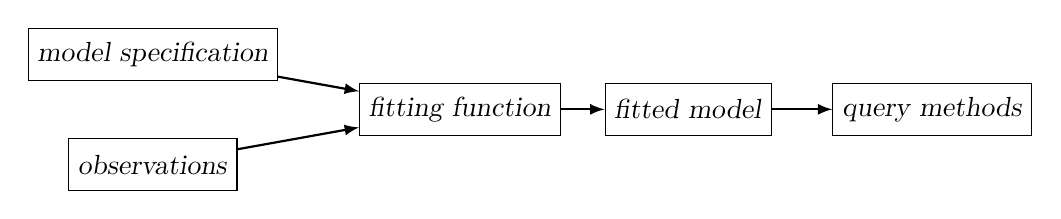
\begin{tikzpicture}[node distance=1.4cm, scale=0.5]
\node (model) [tprocess] {\textsl{model specification}};
\node (data) [tprocess, below of=model] {\textsl{observations}};
\node (fitfun) [tprocess, right of=model, yshift=-0.7cm, xshift=2.5cm] {\textsl{fitting function}};
\node (fm) [tprocess, color = black, right of=fitfun, xshift=1.5cm] {\textsl{fitted model}};
\node (summary) [tprocess, color = black, right of=fm, xshift=1.7cm] {\textsl{query methods}};
\draw [arrow] (model) -- (fitfun);
\draw [arrow] (data) -- (fitfun);
\draw [arrow] (fitfun) -- (fm);
\draw [arrow] (fm) -- (summary);
\end{tikzpicture}
\end{small}
\end{center}

Models are described using model formulas such as \code{y\,\char"007E\,x} which we read as $y$ is explained by $x$. We use \emph{lhs} (left-hand-side) and \emph{rhs} (right-hand-side) to signify all terms to the left and right of the tilde (\code{\,\char"007E\,}), respectively (\code{<lhs>\,\char"007E\,<rhs>}). Model formulas are used in different contexts: fitting of models, plotting, and tests like $t$-test. The syntax of model formulas is consistent throughout base \Rlang and numerous independently developed packages. However, their use is not universal, and several packages extend the basic syntax to allow the description of specific types of models. As most things in \Rlang, model formulas are objects and can be stored in variables. See section \ref{sec:stat:formulas} on page \pageref{sec:stat:formulas} for a detailed discussion of model formulas.

Although there is some variation, especially for fitted model classes defined in extension packages, in most cases the \textsl{query functions} bulked together in the rightmost box in the diagram include methods \Rfunction{summary()}, \Rfunction{anova()} and \Rfunction{plot()}, with several other methods such as \Rfunction{coef()}, \Rfunction{residuals()}, \Rfunction{fitted()}, \Rfunction{predict()}, \Rfunction{AIC()}, \Rfunction{BIC()} usually also available. Additional methods may be available. However, as model fit objects are derived from class \code{list}, these and other components can be extract or computed programmatically when needed. Consequently, the examples in this chapter can be adapted to the fitting of types of models not described here.

\begin{explainbox}
  Fitted model objects in \Rlang are self contained and include a copy of the data to which the model was fit, as well as residuals and possibly even intermediate results of computations. Although this can make the size of these objects large, it allows querying and even updating them in the absence of the data in the current \Rlang workspace.
\end{explainbox}

\index{models fitting|)}

\section{Fitting linear models}\label{sec:stat:LM}
\index{models!linear|see{linear models}}
\index{linear models|(}
\index{LM|see{linear models}}

Regression, analysis of variance (ANOVA) and analysis of covariance (ANCOVA) are all linear models, differing only on the type of explanatory variables included in the statistical model fitted. If in the fitted model all explanatory variables are continuous, i.e., \code{numeric}, vectors, the model is a regression model. If all explanatory variables are discrete, i.e., \code{factors}, the model is ANOVA. Finally, if the model contains but \code{numeric} variables and \code{factors} it is named ANCOVA. As in all cases the fitting approach is the same, based on ordinary least squares (OLS), in \Rlang, they are all implemented in function \Rfunction{lm()}.

There is another meaning of ANOVA, referring only to the tests of significance rather than to an approach to model fitting. Consequently, rather confusingly, results for tests of significance can both in the case of regression, ANOVA and ANCOVA, be presented in an ANOVA table. In this second, stricter meaning, ANOVA means a test of significance based on the ratios between pairs of variances.

\begin{warningbox}
If you do not clearly remember the difference between numeric vectors and factors, or how they can be created, please, revisit chapter \ref{chap:R:as:calc} on page \pageref{chap:R:as:calc}.
\end{warningbox}

The generic diagram from the previous section redrawn to show a linear model fit, done with function \Rfunction{lm()} where the non-filled boxes represent what is in common with the fitting of other types of models, and the filled ones what is specific to \Rfunction{lm()}. The diagram includes only the three most frequently used query methods and both response variables and explanatory variables are included under \textsl{observations} .

\begin{center}
\begin{small}
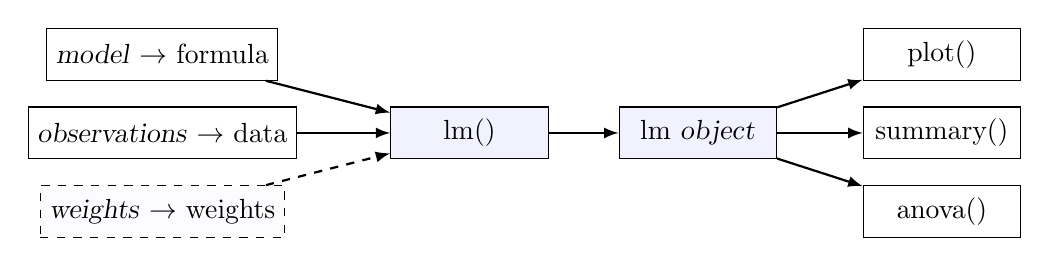
\begin{tikzpicture}[node distance=1.4cm, scale=0.5]
\node (model) [tprocess] {\textsl{model} $\to$ \code{formula}};
\node (data) [tprocess, below of=model, yshift = 0.4cm] {\textsl{observations} $\to$ \code{data}};
\node (weights) [tprocess, dashed, below of=data, fill=blue!1, yshift = 0.4cm] {\textsl{weights} $\to$ \code{weights}};
\node (fitfun) [tprocess, right of=data, xshift=2.5cm, fill=blue!5] {\code{lm()}};
\node (fm) [tprocess, color = black, right of=fitfun, xshift=1.5cm, fill=blue!5] {\code{lm} \textsl{object}};
\node (summary) [tprocess, color = black, right of=fm, xshift=1.7cm] {\code{summary()}};
\node (anova) [tprocess, color = black, below of=summary, yshift = 0.4cm] {\code{anova()}};
\node (plot) [tprocess, color = black, above of=summary, yshift = -0.4cm] {\code{plot()}};
\draw [arrow] (model) -- (fitfun);
\draw [arrow] (data) -- (fitfun);
\draw [arrow, dashed] (weights) -- (fitfun);
\draw [arrow] (fitfun) -- (fm);
\draw [arrow] (fm) -- (plot);
\draw [arrow] (fm) -- (anova);
\draw [arrow] (fm) -- (summary);
\end{tikzpicture}
\end{small}
\end{center}

The observations are stored in a data frame, one case or event per row, with values for both response and explanatory variables in variables or columns. The model formula is used to indicate which variables in the data frame are to be used and in which role: either
response or explanatory, and when explanatory how they contribute to the estimated response.

\begin{explainbox}
Weights are multiplicative factors used to alter the \emph{weight} given to individual residuals when fitting a model to observations that are not equally  informative. A frequent case is fitting a model using \emph{y} or response values that are each a mean calculated from drastically different numbers of individual measurements. Some model fit functions compute the weights, but in most cases they are supplied as an argument to parameter \code{weights}. By default, \code{weights} have a value of \code{1} and thus do not affect the resulting model fit.
\end{explainbox}

\subsection{Regression}
%\index{linear regression}
\index{linear regression|see{linear models, linear regression}}\index{linear models!linear regression}
In this section we continue using the \Rdata{cars} data set, which contains to \code{numeric} variables.

We fit a simple linear model $y = \alpha \cdot 1 + \beta \cdot x$ where $y$ corresponds to stopping distance (\code{dist}) and $x$ to initial speed (\code{speed}). Such a model is formulated in \Rlang as \code{dist \char"007E\ 1 + speed}. We save the fitted model as \code{fm1} (a mnemonic for fitted-model one).\label{chunk:lm:models1}

\begin{knitrout}\footnotesize
\definecolor{shadecolor}{rgb}{1, 1, 1}\color{fgcolor}\begin{kframe}
\begin{alltt}
\hlstd{fm1} \hlkwb{<-} \hlkwd{lm}\hlstd{(dist} \hlopt{~} \hlnum{1} \hlopt{+} \hlstd{speed,} \hlkwc{data}\hlstd{=cars)}
\hlkwd{class}\hlstd{(fm1)}
\end{alltt}
\begin{verbatim}
## [1] "lm"
\end{verbatim}
\end{kframe}
\end{knitrout}

The next step is diagnosis of the fit. Are assumptions of the linear model procedure used reasonably close to being fulfilled? In \Rlang it is most common to use plots to this end. We show here only one of the four plots normally produced. This quantile vs.\ quantile plot allows us to assess how much the residuals deviate from being normally distributed.

\begin{knitrout}\footnotesize
\definecolor{shadecolor}{rgb}{1, 1, 1}\color{fgcolor}\begin{kframe}
\begin{alltt}
\hlkwd{plot}\hlstd{(fm1,} \hlkwc{which} \hlstd{=} \hlnum{2}\hlstd{)}
\end{alltt}
\end{kframe}

{\centering \includegraphics[width=.54\textwidth]{figure/pos-models-1a-1} 

}


\end{knitrout}

In the case of a regression, calling \Rfunction{summary()} with the fitted model object as argument is most useful as it provides a table of coefficient estimates and their errors. Remember that as is the case for most \Rlang functions, the value returned by \Rfunction{summary()} is printed when we call this method at the \Rlang prompt.

\begin{knitrout}\footnotesize
\definecolor{shadecolor}{rgb}{1, 1, 1}\color{fgcolor}\begin{kframe}
\begin{alltt}
\hlkwd{summary}\hlstd{(fm1)}
\end{alltt}
\begin{verbatim}
## 
## Call:
## lm(formula = dist ~ 1 + speed, data = cars)
## 
## Residuals:
##     Min      1Q  Median      3Q     Max 
## -29.069  -9.525  -2.272   9.215  43.201 
## 
## Coefficients:
##             Estimate Std. Error t value Pr(>|t|)    
## (Intercept) -17.5791     6.7584  -2.601   0.0123 *  
## speed         3.9324     0.4155   9.464 1.49e-12 ***
## ---
## Signif. codes:  0 '***' 0.001 '**' 0.01 '*' 0.05 '.' 0.1 ' ' 1
## 
## Residual standard error: 15.38 on 48 degrees of freedom
## Multiple R-squared:  0.6511,	Adjusted R-squared:  0.6438 
## F-statistic: 89.57 on 1 and 48 DF,  p-value: 1.49e-12
\end{verbatim}
\end{kframe}
\end{knitrout}

Let's\index{linear models!summary table} look at the printout of the summary, section by section. Under ``Call:'' we find, \code{dist\ \char"007E\ 1 + speed} or the specification of the model fitted, plus the data used. Under ``Residuals:'' we find the extremes, quartiles and median of the residuals, or deviations between observations and the fitted line. Under ``Coefficients:'' we find the estimates of the model parameters and their variation plus corresponding $t$-tests. At the end of the summary there is information on degrees of freedom and overall coefficient of determination ($R^2$).

If we return to the model formulation, we can now replace $\alpha$ and $\beta$ by the estimates obtaining $y = -17.6 + 3.93 x$. Given the nature of the problem, we \emph{know based on first principles} that stopping distance must be zero when speed is zero. This suggests that we should not estimate the value of $\alpha$ but instead set $\alpha = 0$, or in other words, fit the model $y = \beta \cdot x$.

However, in \Rlang models, the intercept is always implicitly included, so the model fitted above can be formulated as \code{dist\ \char"007E\ speed}---i.e., a missing \code{+ 1} does not change the model. To exclude the intercept from the previous model, we need to specify it as \code{dist\ \char"007E\ speed - 1} (or its equivalent \code{dist\ \char"007E\ speed + 0}), resulting in the fitting of a straight line passing through the origin ($x = 0$, $y = 0$).

Now there is no estimate for the intercept in the summary, only an estimate for the slope.

\begin{knitrout}\footnotesize
\definecolor{shadecolor}{rgb}{1, 1, 1}\color{fgcolor}\begin{kframe}
\begin{alltt}
\hlstd{fm2} \hlkwb{<-} \hlkwd{lm}\hlstd{(dist} \hlopt{~} \hlstd{speed} \hlopt{-} \hlnum{1}\hlstd{,} \hlkwc{data} \hlstd{= cars)}
\hlkwd{summary}\hlstd{(fm2)}
\end{alltt}
\begin{verbatim}
## 
## Call:
## lm(formula = dist ~ speed - 1, data = cars)
## 
## Residuals:
##     Min      1Q  Median      3Q     Max 
## -26.183 -12.637  -5.455   4.590  50.181 
## 
## Coefficients:
##       Estimate Std. Error t value Pr(>|t|)    
## speed   2.9091     0.1414   20.58   <2e-16 ***
## ---
## Signif. codes:  0 '***' 0.001 '**' 0.01 '*' 0.05 '.' 0.1 ' ' 1
## 
## Residual standard error: 16.26 on 49 degrees of freedom
## Multiple R-squared:  0.8963,	Adjusted R-squared:  0.8942 
## F-statistic: 423.5 on 1 and 49 DF,  p-value: < 2.2e-16
\end{verbatim}
\end{kframe}
\end{knitrout}

The equation of the second fitted model is $y = 2.91 x$, and from the residuals, it can be seen that it is inadequate, as the straight line does not follow the curvature of the relationship between \code{dist} and \code{speed}.

\begin{playground}
You will now fit a second-degree polynomial\index{linear models!polynomial regression}\index{polynomial regression}, a different linear model: $y = \alpha \cdot 1 + \beta_1 \cdot x + \beta_2 \cdot x^2$. The function used is the same as for linear regression, \Rfunction{lm()}. We only need to alter the formulation of the model. The identity function \Rfunction{I()} is used to protect its argument from being interpreted as part of the model formula. Instead, its argument is evaluated beforehand and the result is used as the, in this case second, explanatory variable.\label{chunk:stats:fm3}

\begin{knitrout}\footnotesize
\definecolor{shadecolor}{rgb}{1, 1, 1}\color{fgcolor}\begin{kframe}
\begin{alltt}
\hlstd{fm3} \hlkwb{<-} \hlkwd{lm}\hlstd{(dist} \hlopt{~} \hlstd{speed} \hlopt{+} \hlkwd{I}\hlstd{(speed}\hlopt{^}\hlnum{2}\hlstd{),} \hlkwc{data} \hlstd{= cars)}
\hlkwd{plot}\hlstd{(fm3,} \hlkwc{which} \hlstd{=} \hlnum{3}\hlstd{)}
\hlkwd{summary}\hlstd{(fm3)}
\hlkwd{anova}\hlstd{(fm3)}
\end{alltt}
\end{kframe}
\end{knitrout}

The ``same'' fit using an orthogonal polynomial can be specified using function \Rfunction{poly()}. Polynomials of different degrees can be obtained by supplying as the second argument to \Rfunction{poly()} the corresponding positive integer value. In this case, the different terms of the polynomial are bulked together in the summary.

\begin{knitrout}\footnotesize
\definecolor{shadecolor}{rgb}{1, 1, 1}\color{fgcolor}\begin{kframe}
\begin{alltt}
\hlstd{fm3a} \hlkwb{<-} \hlkwd{lm}\hlstd{(dist} \hlopt{~} \hlkwd{poly}\hlstd{(speed,} \hlnum{2}\hlstd{),} \hlkwc{data} \hlstd{= cars)}
\hlkwd{summary}\hlstd{(fm3a)}
\hlkwd{anova}\hlstd{(fm3a)}
\end{alltt}
\end{kframe}
\end{knitrout}

We can also compare two model fits using \Rfunction{anova()}, to test whether one of the models describes the data better than the other. It is important in this case to take into consideration the nature of the difference between the model formulas, most importantly if they can be interpreted as nested---i.e., interpreted as a base model vs. the same model with additional terms.

\begin{knitrout}\footnotesize
\definecolor{shadecolor}{rgb}{1, 1, 1}\color{fgcolor}\begin{kframe}
\begin{alltt}
\hlkwd{anova}\hlstd{(fm2, fm1)}
\end{alltt}
\end{kframe}
\end{knitrout}

Three or more models can also be compared in a single call to \Rfunction{anova()}. However, be careful, as the order of the arguments matters.

\begin{knitrout}\footnotesize
\definecolor{shadecolor}{rgb}{1, 1, 1}\color{fgcolor}\begin{kframe}
\begin{alltt}
\hlkwd{anova}\hlstd{(fm2, fm3, fm3a)}
\hlkwd{anova}\hlstd{(fm2, fm3a, fm3)}
\end{alltt}
\end{kframe}
\end{knitrout}

\label{par:stats:AIC}%
We\index{Akaike's An Information Criterion@Akaike's \emph{An Information Criterion}}\index{AIC|see \emph{An Information Criterion}}%
\index{Bayesian Information Criterion@\emph{Bayesian Information Criterion}}\index{BIC|see \emph{Bayesian Information Criterion}}%
\index{Schwarz's Bayesian criterion@\emph{Schwarz's Bayesian criterion}|see \emph{Bayesian Information Criterion}} can use different criteria to choose the ``best'' model: significance based on $p$-values or information criteria (AIC, BIC). AIC (Akaike's ``An Information Criterion'') and BIC (``Bayesian Information Criterion'' = SBC, ``Schwarz's Bayesian criterion'') that penalize the resulting ``goodness'' based on the number of parameters in the fitted model. In the case of AIC and BIC, a smaller value is better, and values returned can be either positive or negative, in which case more negative is better. Estimates for both BIC and AIC are returned by \Rfunction{anova()}, and on their own by \Rfunction{BIC()} and \Rfunction{AIC()}

\begin{knitrout}\footnotesize
\definecolor{shadecolor}{rgb}{1, 1, 1}\color{fgcolor}\begin{kframe}
\begin{alltt}
\hlkwd{BIC}\hlstd{(fm2, fm1, fm3, fm3a)}
\hlkwd{AIC}\hlstd{(fm2, fm1, fm3, fm3a)}
\end{alltt}
\end{kframe}
\end{knitrout}

Once you have run the code in the chunks above, you will be able see that these three criteria do not necessarily agree on which is the ``best'' model. Find in the output $p$-value, BIC and AIC estimates, for the different models and conclude which model is favored by each of the three criteria. In addition you will notice that the two different formulations of the quadratic polynomial are equivalent.

\end{playground}

Additional methods give easy access to different components of fitted models: \Rfunction{vcov()} returns the variance-covariance matrix, \Rfunction{coef()} and its alias \Rfunction{coefficients()} return the estimates for the fitted model coefficients, \Rfunction{fitted()} and its alias \Rfunction{fitted.values()} extract the fitted values, and \Rfunction{resid()} and its alias \Rfunction{residuals()} the corresponding residuals (or deviations). Less frequently used accessors are \Rfunction{getCall()}, \Rfunction{effects()}, \Rfunction{terms()}, \Rfunction{model.frame()} and \Rfunction{model.matrix()}. The diagram below shows how some of these methods fit in the model fitting workflow.

\begin{center}
\begin{small}
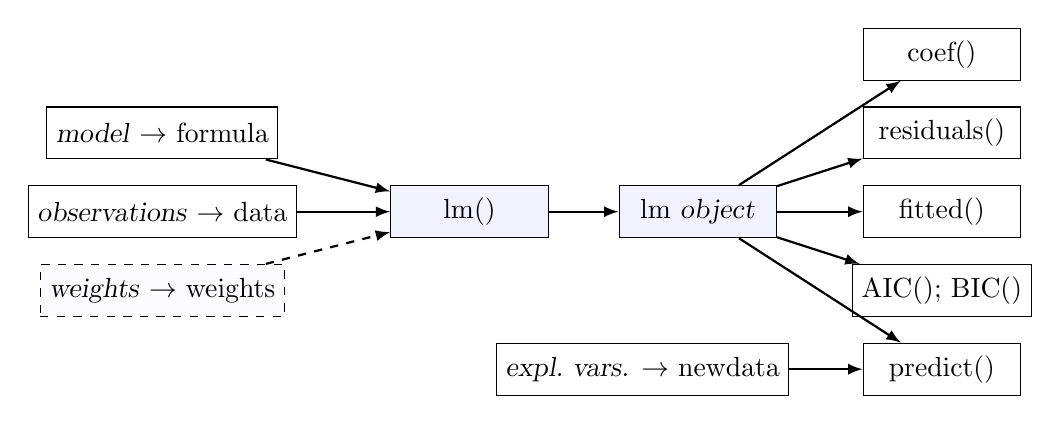
\begin{tikzpicture}[node distance=1.4cm, scale=0.5]
\node (model) [tprocess] {\textsl{model} $\to$ \code{formula}};
\node (data) [tprocess, below of=model, yshift = 0.4cm] {\textsl{observations} $\to$ \code{data}};
\node (weights) [tprocess, dashed, below of=data, fill=blue!1, yshift = 0.4cm] {\textsl{weights} $\to$ \code{weights}};
\node (fitfun) [tprocess, right of=data, xshift=2.5cm, fill=blue!5] {\code{lm()}};
\node (fm) [tprocess, color = black, right of=fitfun, xshift=1.5cm, fill=blue!5] {\code{lm} \textsl{object}};
\node (fitted) [tprocess, color = black, right of=fm, xshift=1.7cm] {\code{fitted()}};
\node (resid) [tprocess, color = black, above of=fitted, yshift = -0.4cm] {\code{residuals()}};
\node (coef) [tprocess, color = black, above of=resid, yshift = -0.4cm] {\code{coef()}};
\node (aic) [tprocess, color = black, below of=fitted, yshift = 0.4cm] {\code{AIC()}; \code{BIC()}};
\node (predict) [tprocess, color = black, below of=aic, yshift = 0.4cm] {\code{predict()}};
\node (newdata) [tprocess, color = black, left of=predict, xshift = -2.4cm] {\textsl{expl.\ vars.} $\to$ \code{newdata}};
\draw [arrow] (model) -- (fitfun);
\draw [arrow] (data) -- (fitfun);
\draw [arrow, dashed] (weights) -- (fitfun);
\draw [arrow] (fitfun) -- (fm);
\draw [arrow] (fm) -- (coef);
\draw [arrow] (fm) -- (resid);
\draw [arrow] (fm) -- (fitted);
\draw [arrow] (fm) -- (aic);
\draw [arrow] (fm) -- (predict);
\draw [arrow] (newdata) -- (predict);
\end{tikzpicture}
\end{small}
\end{center}

\begin{playground}
Familiarize yourself with these extraction and summary methods by reading their documentation and use them to explore \code{fm1} fitted above or model fits to other data of your interest.
\end{playground}

\begin{explainbox}\label{box:LM:fit:object}
The\index{linear models!structure of model fit object} objects returned by model fitting functions contain the full information, including the data to which the model was fit to. Their structure resembles a nested list. In most cases the class of the objects returned by model fit functions agrees in name with the name of the model-fit function (\code{"lm"} in this example) but is not derived from \Rlang class \code{"list"}. The different functions described above, either extract parts of the object or do additional calculations and formatting based on them. There are different specializations of these methods which are called depending on the class of the model-fit object. (See section \ref{sec:methods} on page \pageref{sec:methods}.)

\begin{knitrout}\footnotesize
\definecolor{shadecolor}{rgb}{1, 1, 1}\color{fgcolor}\begin{kframe}
\begin{alltt}
\hlkwd{class}\hlstd{(fm1)}
\end{alltt}
\begin{verbatim}
## [1] "lm"
\end{verbatim}
\begin{alltt}
\hlkwd{names}\hlstd{(fm1)}
\end{alltt}
\begin{verbatim}
##  [1] "coefficients"  "residuals"     "effects"       "rank"         
##  [5] "fitted.values" "assign"        "qr"            "df.residual"  
##  [9] "xlevels"       "call"          "terms"         "model"
\end{verbatim}
\end{kframe}
\end{knitrout}

We rarely need to manually explore the structure of these model-fit objects when using \Rlang interactively. In contrast, when including model fitting in scripts or package code, the need to efficiently extract specific members from them can be useful. As with any other \Rlang object we can use \Rfunction{str()} to explore them. As this prints as a long text, we call \Rfunction{str()} with options that restrict the output to get an overall view of the structure of \code{fm1}. Later as an example, we look in detail two components of the \code{fm1} object and leave to the reader the task of exploring the remaining ones.

\begin{knitrout}\footnotesize
\definecolor{shadecolor}{rgb}{1, 1, 1}\color{fgcolor}\begin{kframe}
\begin{alltt}
\hlkwd{str}\hlstd{(fm1,} \hlkwc{no.list} \hlstd{=} \hlnum{TRUE}\hlstd{,} \hlkwc{give.attr} \hlstd{=} \hlnum{FALSE}\hlstd{,} \hlkwc{vec.len} \hlstd{=} \hlnum{2}\hlstd{)}
\end{alltt}
\begin{verbatim}
##  $ coefficients : Named num [1:2] -17.58 3.93
##  $ residuals    : Named num [1:50] 3.85 11.85 ...
##  $ effects      : Named num [1:50] -304 146 ...
##  $ rank         : int 2
##  $ fitted.values: Named num [1:50] -1.85 -1.85 ...
##  $ assign       : int [1:2] 0 1
##  $ qr           :List of 5
##   ..$ qr   : num [1:50, 1:2] -7.071 0.141 ...
##   ..$ qraux: num [1:2] 1.14 1.27
##   ..$ pivot: int [1:2] 1 2
##   ..$ tol  : num 1e-07
##   ..$ rank : int 2
##  $ df.residual  : int 48
##  $ xlevels      : Named list()
##  $ call         : language lm(formula = dist ~ 1 + speed, data = cars)
##  $ terms        :Classes 'terms', 'formula'  language dist ~ 1 + speed
##  $ model        :'data.frame':	50 obs. of  2 variables:
##   ..$ dist : num [1:50] 2 10 4 22 16 ...
##   ..$ speed: num [1:50] 4 4 7 7 8 ...
\end{verbatim}
\end{kframe}
\end{knitrout}

Under \code{call} we find the function call that returned the value we saved to the \code{fm1} object.

\begin{knitrout}\footnotesize
\definecolor{shadecolor}{rgb}{1, 1, 1}\color{fgcolor}\begin{kframe}
\begin{alltt}
\hlkwd{str}\hlstd{(fm1}\hlopt{$}\hlstd{call)}
\end{alltt}
\begin{verbatim}
##  language lm(formula = dist ~ 1 + speed, data = cars)
\end{verbatim}
\end{kframe}
\end{knitrout}

We\index{linear models!structure of summary object} frequently only look at the output of \Rfunction{anova()} and \Rfunction{summary()} as implicitly displayed by \code{print()}. However, both \Rfunction{anova()} and \Rfunction{summary()} return complex objects, derived from \code{list}, containing additional component members not displayed by the matching \code{print()} methods. Access to the components of these objects tends to be more frequently useful than to the components of model fit objects.

The class of the object returned by \code{anova()} does not depend on the class of the model fit object, while its structure does depend.

\begin{knitrout}\footnotesize
\definecolor{shadecolor}{rgb}{1, 1, 1}\color{fgcolor}\begin{kframe}
\begin{alltt}
\hlkwd{anova}\hlstd{(fm1)}
\end{alltt}
\begin{verbatim}
## Analysis of Variance Table
## 
## Response: dist
##           Df Sum Sq Mean Sq F value   Pr(>F)    
## speed      1  21186 21185.5  89.567 1.49e-12 ***
## Residuals 48  11354   236.5                     
## ---
## Signif. codes:  0 '***' 0.001 '**' 0.01 '*' 0.05 '.' 0.1 ' ' 1
\end{verbatim}
\end{kframe}
\end{knitrout}

\begin{knitrout}\footnotesize
\definecolor{shadecolor}{rgb}{1, 1, 1}\color{fgcolor}\begin{kframe}
\begin{alltt}
\hlkwd{class}\hlstd{(}\hlkwd{anova}\hlstd{(fm1))}
\end{alltt}
\begin{verbatim}
## [1] "anova"      "data.frame"
\end{verbatim}
\end{kframe}
\end{knitrout}

\begin{knitrout}\footnotesize
\definecolor{shadecolor}{rgb}{1, 1, 1}\color{fgcolor}\begin{kframe}
\begin{alltt}
\hlkwd{str}\hlstd{(}\hlkwd{anova}\hlstd{(fm1))}
\end{alltt}
\begin{verbatim}
## Classes 'anova' and 'data.frame':	2 obs. of  5 variables:
##  $ Df     : int  1 48
##  $ Sum Sq : num  21185 11354
##  $ Mean Sq: num  21185 237
##  $ F value: num  89.6 NA
##  $ Pr(>F) : num  1.49e-12 NA
##  - attr(*, "heading")= chr [1:2] "Analysis of Variance Table\n" "Response: dist"
\end{verbatim}
\end{kframe}
\end{knitrout}

The class of the summary objects depends on the class of the model fit object; \Rfunction{summary()} is a generic method with multiple specializations.

\begin{knitrout}\footnotesize
\definecolor{shadecolor}{rgb}{1, 1, 1}\color{fgcolor}\begin{kframe}
\begin{alltt}
\hlkwd{class}\hlstd{(}\hlkwd{summary}\hlstd{(fm1))}
\end{alltt}
\begin{verbatim}
## [1] "summary.lm"
\end{verbatim}
\end{kframe}
\end{knitrout}

Knowing that these objects contain additional information can be very useful, for example, when we want to display the results from the fit in a different format or to implement additional tests or computations. One case is adding annotations to plots and another is when writing reports to include programmatically the computed values within the text. Once again we use \Rfunction{str()} to look at the structure in a simplified way, and later at one member as example.

\begin{knitrout}\footnotesize
\definecolor{shadecolor}{rgb}{1, 1, 1}\color{fgcolor}\begin{kframe}
\begin{alltt}
\hlkwd{str}\hlstd{(}\hlkwd{summary}\hlstd{(fm1),} \hlkwc{no.list} \hlstd{=} \hlnum{TRUE}\hlstd{,} \hlkwc{give.attr} \hlstd{=} \hlnum{FALSE}\hlstd{,} \hlkwc{vec.len} \hlstd{=} \hlnum{2}\hlstd{)}
\end{alltt}
\begin{verbatim}
##  $ call         : language lm(formula = dist ~ 1 + speed, data = cars)
##  $ terms        :Classes 'terms', 'formula'  language dist ~ 1 + speed
##  $ residuals    : Named num [1:50] 3.85 11.85 ...
##  $ coefficients : num [1:2, 1:4] -17.58 3.93 ...
##  $ aliased      : Named logi [1:2] FALSE FALSE
##  $ sigma        : num 15.4
##  $ df           : int [1:3] 2 48 2
##  $ r.squared    : num 0.651
##  $ adj.r.squared: num 0.644
##  $ fstatistic   : Named num [1:3] 89.6 1 ...
##  $ cov.unscaled : num [1:2, 1:2] 0.1931 -0.0112 ...
\end{verbatim}
\end{kframe}
\end{knitrout}

Once we know the structure of the object and the names of members, we can simply extract them using the usual \Rlang rules for member extraction.

\begin{knitrout}\footnotesize
\definecolor{shadecolor}{rgb}{1, 1, 1}\color{fgcolor}\begin{kframe}
\begin{alltt}
\hlkwd{summary}\hlstd{(fm1)}\hlopt{$}\hlstd{adj.r.squared}
\end{alltt}
\begin{verbatim}
## [1] 0.6438102
\end{verbatim}
\end{kframe}
\end{knitrout}

We can also explore the structure of individual members. The \code{coefficients} estimates in the summary are accompanied by estimates for the corresponding standard errors, \emph{t}-value and \emph{P}-value estimates, while in the model object \code{fm1} the additional estimates are not included.

\begin{knitrout}\footnotesize
\definecolor{shadecolor}{rgb}{1, 1, 1}\color{fgcolor}\begin{kframe}
\begin{alltt}
\hlkwd{coef}\hlstd{(fm1)}
\end{alltt}
\begin{verbatim}
## (Intercept)       speed 
##  -17.579095    3.932409
\end{verbatim}
\begin{alltt}
\hlkwd{str}\hlstd{(fm1}\hlopt{$}\hlstd{coefficients)}
\end{alltt}
\begin{verbatim}
##  Named num [1:2] -17.58 3.93
##  - attr(*, "names")= chr [1:2] "(Intercept)" "speed"
\end{verbatim}
\begin{alltt}
\hlkwd{print}\hlstd{(}\hlkwd{summary}\hlstd{(fm1)}\hlopt{$}\hlstd{coefficients)}
\end{alltt}
\begin{verbatim}
##               Estimate Std. Error   t value     Pr(>|t|)
## (Intercept) -17.579095  6.7584402 -2.601058 1.231882e-02
## speed         3.932409  0.4155128  9.463990 1.489836e-12
\end{verbatim}
\begin{alltt}
\hlkwd{str}\hlstd{(}\hlkwd{summary}\hlstd{(fm1)}\hlopt{$}\hlstd{coefficients)}
\end{alltt}
\begin{verbatim}
##  num [1:2, 1:4] -17.579 3.932 6.758 0.416 -2.601 ...
##  - attr(*, "dimnames")=List of 2
##   ..$ : chr [1:2] "(Intercept)" "speed"
##   ..$ : chr [1:4] "Estimate" "Std. Error" "t value" "Pr(>|t|)"
\end{verbatim}
\end{kframe}
\end{knitrout}

\end{explainbox}

\begin{advplayground}
As\index{linear models!test parameters for $H_0 \neq 0$} an example of the use of values extracted from the \code{summary.lm} object, we test if the slope from a linear regression fit deviates significantly from a constant value different from the usual zero. A null hypothesis of zero for the slope tests for the presence of an ``effect'' of an explanatory variable, which is usually of interest in an experiment. In contrast, when testing for deviations from a calibration by comparing two instruments or an instrument and a reference, a null hypothesis of one for the slope will test for deviations from the true readings. In some cases, we may want to test if the estimate for a parameter exceeds some other value, such as acceptable product tolerances. In other cases, when comparing the effectiveness of interventions we may be interested to test if a new approach surpasses that in current use by at least a specific margin. There exist many situations where the question of interest is not that an effect deviates from zero. Furthermore, when dealing with big data, very small deviations from zero can be statistically significant but biologically or practically irrelevant. In such case we can set the smallest response that is of interest, instead of zero, as the null hypothesis in the test.

The examples above, using \Rfunction{anova()} and \Rfunction{summary()} are for a null hypothesis of slope = 0. Here we do the equivalent test with a null hypothesis of slope = 1. The procedure is applicable to any constant value as a null hypothesis for any of the fitted parameter estimates. However, for the $P$-value estimates to be valid, the hypotheses should be set in advance of the study, i.e., independent of the observations used for the test. The examples use a two-sided test. In some cases, a single-sided test should be used (e.g., if its known a priori because of physical reasons that deviation is possible only in one direction away from the null hypothesis, or because only one direction of response is of interest).

To estimate the \emph{t}-value we need an estimate for the parameter value and an estimate of the standard error for this estimate, and the degrees of freedom. We can extract all these values from the summary of a fitted model object.

\begin{knitrout}\footnotesize
\definecolor{shadecolor}{rgb}{1, 1, 1}\color{fgcolor}\begin{kframe}
\begin{alltt}
\hlstd{est.slope.value} \hlkwb{<-} \hlkwd{summary}\hlstd{(fm1)}\hlopt{$}\hlstd{coefficients[}\hlstr{"speed"}\hlstd{,} \hlstr{"Estimate"}\hlstd{]}
\hlstd{est.slope.se} \hlkwb{<-} \hlkwd{summary}\hlstd{(fm1)}\hlopt{$}\hlstd{coefficients[}\hlstr{"speed"}\hlstd{,} \hlstr{"Std. Error"}\hlstd{]}
\hlstd{degrees.of.freedom} \hlkwb{<-} \hlkwd{summary}\hlstd{(fm1)}\hlopt{$}\hlstd{df[}\hlnum{2}\hlstd{]}
\end{alltt}
\end{kframe}
\end{knitrout}

A new \emph{t}-value is computed based on the difference between the value of the null hypothesis and the value for the parameter estimated from the observations. A new probability estimate is computed based on computed $t$-value, or quantile, and the $t$ distribution with matching degrees of freedom with a call to \Rfunction{pt()} (see section \ref{sec:prob:dist} on page \pageref{sec:prob:dist}.) For a two-tails test we multiply by two the one-tail $P$ estimate.

\begin{knitrout}\footnotesize
\definecolor{shadecolor}{rgb}{1, 1, 1}\color{fgcolor}\begin{kframe}
\begin{alltt}
\hlstd{hyp.null} \hlkwb{<-} \hlnum{1}
\hlstd{t.value} \hlkwb{<-} \hlstd{(est.slope.value} \hlopt{-} \hlstd{hyp.null)} \hlopt{/} \hlstd{est.slope.se}
\hlstd{p.value} \hlkwb{<-} \hlnum{2} \hlopt{*} \hlkwd{pt}\hlstd{(}\hlkwc{q} \hlstd{= t.value,} \hlkwc{df} \hlstd{= degrees.of.freedom,} \hlkwc{lower.tail} \hlstd{=} \hlnum{FALSE}\hlstd{)}
\hlkwd{cat}\hlstd{(}\hlstr{"slope ="}\hlstd{,} \hlkwd{signif}\hlstd{(est.slope.value,} \hlnum{3}\hlstd{),} \hlstr{"with s.e. ="}\hlstd{,} \hlkwd{signif}\hlstd{(est.slope.se,} \hlnum{3}\hlstd{),}
    \hlstr{"\textbackslash{}nt.value ="}\hlstd{,} \hlkwd{signif}\hlstd{(t.value,} \hlnum{3}\hlstd{),} \hlstr{"and P-value ="}\hlstd{,} \hlkwd{signif}\hlstd{(p.value,} \hlnum{3}\hlstd{))}
\end{alltt}
\begin{verbatim}
## slope = 3.93 with s.e. = 0.416 
## t.value = 7.06 and P-value = 6.01e-09
\end{verbatim}
\end{kframe}
\end{knitrout}

This example is for a linear model fitted with function \Rfunction{lm()} but the same approach can be applied to other model fit procedures for which parameter estimates and their corresponding standard error estimates can be extracted or computed.

Check that the procedure above agrees with the output of \code{summary()} when we set \code{hyp.null <- 0} instead of \code{hyp.null <- 1} in our code.

Modify the example above so as to test whether the intercept is significantly larger than 5 feet, doing a one-sided test.

Use \code{class(anova(fm1))} and \code{str(anova(fm1))} to explore the \Rlang object returned by the call \code{anova(fm1)}.

\end{advplayground}

Method \Rfunction{predict()} uses the fitted model together with new data for the independent variables to compute predictions. As \Rfunction{predict()} accepts new data as input, it allows interpolation and extrapolation to values of the independent variables not present in the original data. In the case of fits of linear- and some other models, method \Rfunction{predict()} returns, in addition to the prediction, estimates of the confidence and/or prediction intervals. The new data must be stored in a data frame with columns using the same names for the explanatory variables as in the data used for the fit, a response variable is not needed and additional columns are ignored. (The explanatory variables in the new data can be either continuous or factors, but they must match in this respect those in the original data.)

\begin{infobox}
  Method \Rfunction{predict()} is behind most plotting of lines corresponding to fitted models. For some types of models plotting is automated by ready available methods that both generate the predicted values and plot them. In other cases it is necessary to generate the predicted values with \Rfunction{predict()} and use these values as data input for a line-plotting method.
\end{infobox}

\begin{playground}
Predict using both \code{fm1} and \code{fm2} the distance required to stop cars moving at 0, 5, 10, 20, 30, and 40~mph. Study the help page for the predict method for linear models (using \code{help(predict.lm)}). Explore the difference between \code{"prediction"} and \code{"confidence"} bands: why are they so different?
\end{playground}

\subsection{Analysis of variance, ANOVA}\label{sec:anova}
%\index{analysis of variance}
\index{analysis of variance|see{linear models, analysis of variance}}\index{linear models!analysis of variance}
\index{ANOVA|see{linear models, analysis of variance}}
We use here the \Rdata{InsectSprays} data set, giving insect counts in plots sprayed with different insecticides. In these data, \code{spray} is a factor with six levels.%
\label{xmpl:fun:lm:fm4}

The call is exactly the same as the one for linear regression, only the names of the variables and data frame are different. What determines that this is an ANOVA is that \code{spray}, the explanatory variable, is a \code{factor}.

\begin{knitrout}\footnotesize
\definecolor{shadecolor}{rgb}{1, 1, 1}\color{fgcolor}\begin{kframe}
\begin{alltt}
\hlkwd{data}\hlstd{(InsectSprays)}
\hlkwd{is.numeric}\hlstd{(InsectSprays}\hlopt{$}\hlstd{spray)}
\end{alltt}
\begin{verbatim}
## [1] FALSE
\end{verbatim}
\begin{alltt}
\hlkwd{is.factor}\hlstd{(InsectSprays}\hlopt{$}\hlstd{spray)}
\end{alltt}
\begin{verbatim}
## [1] TRUE
\end{verbatim}
\begin{alltt}
\hlkwd{levels}\hlstd{(InsectSprays}\hlopt{$}\hlstd{spray)}
\end{alltt}
\begin{verbatim}
## [1] "A" "B" "C" "D" "E" "F"
\end{verbatim}
\end{kframe}
\end{knitrout}

We fit the model in exactly the same way as for linear regression; the difference is that we use a factor as the explanatory variable. By using a factor instead of a numeric vector, a different model matrix is built from an equivalent formula.\label{chunk:stat:fm4}

\begin{knitrout}\footnotesize
\definecolor{shadecolor}{rgb}{1, 1, 1}\color{fgcolor}\begin{kframe}
\begin{alltt}
\hlstd{fm4} \hlkwb{<-} \hlkwd{lm}\hlstd{(count} \hlopt{~} \hlstd{spray,} \hlkwc{data} \hlstd{= InsectSprays)}
\end{alltt}
\end{kframe}
\end{knitrout}

Diagnostic plots are obtained in the same way as for linear regression.

\begin{knitrout}\footnotesize
\definecolor{shadecolor}{rgb}{1, 1, 1}\color{fgcolor}\begin{kframe}
\begin{alltt}
\hlkwd{plot}\hlstd{(fm4,} \hlkwc{which} \hlstd{=} \hlnum{3}\hlstd{)}
\end{alltt}
\end{kframe}

{\centering \includegraphics[width=.54\textwidth]{figure/pos-model-6a-1} 

}


\end{knitrout}

In ANOVA we are mainly interested in testing hypotheses, and \Rfunction{anova()} provides the most interesting output. Function \Rfunction{summary()} can be used to extract parameter estimates. The default contrasts and corresponding $p$-values returned by \Rfunction{summary()} test hypotheses that have little or no direct interest in an analysis of variance. Function \Rfunction{aov()} is a wrapper on \Rfunction{lm()} that returns an object that by default when printed displays the output of \Rfunction{anova()}.

\begin{knitrout}\footnotesize
\definecolor{shadecolor}{rgb}{1, 1, 1}\color{fgcolor}\begin{kframe}
\begin{alltt}
\hlkwd{anova}\hlstd{(fm4)}
\end{alltt}
\begin{verbatim}
## Analysis of Variance Table
## 
## Response: count
##           Df Sum Sq Mean Sq F value    Pr(>F)    
## spray      5 2668.8  533.77  34.702 < 2.2e-16 ***
## Residuals 66 1015.2   15.38                      
## ---
## Signif. codes:  0 '***' 0.001 '**' 0.01 '*' 0.05 '.' 0.1 ' ' 1
\end{verbatim}
\end{kframe}
\end{knitrout}

\begin{warningbox}
The defaults used for model fits and ANOVA calculations vary among programs. There exist different so-called ``types'' of sums of squares, usually called I, II, and III. In orthogonal designs the choice has no consequences, but differences can be important for unbalanced designs, even leading to different conclusions. \Rlang's default, type~I, is usually considered to suffer milder problems than type~III, the default used by \pgrmname{SPSS} and \pgrmname{SAS}.
\end{warningbox}

\index{linear models!contrasts|(}
\begin{warningbox}
The contrasts used affect the estimates returned by \Rfunction{coef()} and \Rfunction{summary()} applied to an ANOVA model fit. The default used in \Rlang is different to that used in some other programs (even different than in \Slang). The default, \code{contr.treatment} uses the first level of the factor (assumed to be a control) as reference for estimation of coefficients and testing of their significance. Instead, \code{contr.sum} uses as reference the mean of all levels, i.e., using as condition that the sum of the coefficient estimates is equal to zero. Obviously this changes what the coefficients describe, and consequently also the estimated $p$-values, and most importantly how the result of the tests should be interpreted.
\end{warningbox}

The most straightforward way of setting a different default for a whole series of model fits is by setting \Rlang option \code{contrasts}, which we here only print.

\begin{knitrout}\footnotesize
\definecolor{shadecolor}{rgb}{1, 1, 1}\color{fgcolor}\begin{kframe}
\begin{alltt}
\hlkwd{options}\hlstd{(}\hlstr{"contrasts"}\hlstd{)}
\end{alltt}
\begin{verbatim}
## $contrasts
##         unordered           ordered 
## "contr.treatment"      "contr.poly"
\end{verbatim}
\end{kframe}
\end{knitrout}

The option is set to a named character vector of length two, with the first value, named \code{unordered} giving the name of the function used when the explanatory variable is an unordered factor (created with \Rfunction{factor()}) and the second value, named \code{ordered}, giving the name of the function used when the explanatory variable is an ordered factor (created with \Rfunction{ordered()}).

It is also possible to select the contrast to be used in the call to \code{aov()} or \code{lm()}.

\begin{knitrout}\footnotesize
\definecolor{shadecolor}{rgb}{1, 1, 1}\color{fgcolor}\begin{kframe}
\begin{alltt}
\hlstd{fm4trea} \hlkwb{<-} \hlkwd{lm}\hlstd{(count} \hlopt{~} \hlstd{spray,} \hlkwc{data} \hlstd{= InsectSprays,}
              \hlkwc{contrasts} \hlstd{=} \hlkwd{list}\hlstd{(}\hlkwc{spray} \hlstd{= contr.treatment))}
\hlstd{fm4sum}  \hlkwb{<-} \hlkwd{lm}\hlstd{(count} \hlopt{~} \hlstd{spray,} \hlkwc{data} \hlstd{= InsectSprays,}
              \hlkwc{contrasts} \hlstd{=} \hlkwd{list}\hlstd{(}\hlkwc{spray} \hlstd{= contr.sum))}
\end{alltt}
\end{kframe}
\end{knitrout}

Interpretation of any analysis has to take into account these differences and users should not be surprised if ANOVA yields different results in base \Rlang and \pgrmname{SPSS} or \pgrmname{SAS} given the different types of sums of squares used. The interpretation of ANOVA on designs that are not orthogonal will depend on which type is used, so the different results are not necessarily contradictory even when different.

In \code{fm4trea} we used \Rfunction{contr.treatment()}, thus contrasts for individual treatments are done against \code{Spray1} taking it as the control or reference, and can be inferred from the generated contrasts matrix. For this reason, there is no row for \code{Spray1} in the summary table. Each of the rows \code{Spray2} to \code{Spray6} is a test comparing these treatments individually against \code{Spray1}.

\begin{warningbox}
  Contrast are specified as matrices that are constructed by functions based on the number of levels in a factor. Constructor function \Rfunction{contr.treatment()} is the default in \Rlang for unordered factors, constructor \Rfunction{contr.SAS()} mimics the contrasts used in many \pgrmname{SAS} procedures, and \Rfunction{contr.helmert()} matches the default in \pgrmname{S}. Contrasts depend on the order of factor levels so it is crucial to ensure that the ordering in use yields the intended tests of significance for individual parameter estimates. (How to change the order of factor levels is explained in section \ref{sec:calc:factors} on page \pageref{sec:calc:factors}.)
\end{warningbox}

\begin{knitrout}\footnotesize
\definecolor{shadecolor}{rgb}{1, 1, 1}\color{fgcolor}\begin{kframe}
\begin{alltt}
\hlkwd{contr.treatment}\hlstd{(}\hlkwd{length}\hlstd{(}\hlkwd{levels}\hlstd{(InsectSprays}\hlopt{$}\hlstd{spray)))}
\end{alltt}
\begin{verbatim}
##   2 3 4 5 6
## 1 0 0 0 0 0
## 2 1 0 0 0 0
## 3 0 1 0 0 0
## 4 0 0 1 0 0
## 5 0 0 0 1 0
## 6 0 0 0 0 1
\end{verbatim}
\end{kframe}
\end{knitrout}

\begin{knitrout}\footnotesize
\definecolor{shadecolor}{rgb}{1, 1, 1}\color{fgcolor}\begin{kframe}
\begin{alltt}
\hlkwd{summary}\hlstd{(fm4trea)}
\end{alltt}
\begin{verbatim}
## 
## Call:
## lm(formula = count ~ spray, data = InsectSprays, contrasts = list(spray = contr.treatment))
## 
## Residuals:
##    Min     1Q Median     3Q    Max 
## -8.333 -1.958 -0.500  1.667  9.333 
## 
## Coefficients:
##             Estimate Std. Error t value Pr(>|t|)    
## (Intercept)  14.5000     1.1322  12.807  < 2e-16 ***
## sprayB        0.8333     1.6011   0.520    0.604    
## sprayC      -12.4167     1.6011  -7.755 7.27e-11 ***
## sprayD       -9.5833     1.6011  -5.985 9.82e-08 ***
## sprayE      -11.0000     1.6011  -6.870 2.75e-09 ***
## sprayF        2.1667     1.6011   1.353    0.181    
## ---
## Signif. codes:  0 '***' 0.001 '**' 0.01 '*' 0.05 '.' 0.1 ' ' 1
## 
## Residual standard error: 3.922 on 66 degrees of freedom
## Multiple R-squared:  0.7244,	Adjusted R-squared:  0.7036 
## F-statistic:  34.7 on 5 and 66 DF,  p-value: < 2.2e-16
\end{verbatim}
\end{kframe}
\end{knitrout}

In \code{fm4sum} we used \Rfunction{contr.sum()}, thus contrasts for individual treatments are done differently, as can be inferred from the contrasts matrix. The sum is constrained to be zero, thus estimates for the last treatment level are determined by the sum of the previous ones, and not tested for significance.

\begin{knitrout}\footnotesize
\definecolor{shadecolor}{rgb}{1, 1, 1}\color{fgcolor}\begin{kframe}
\begin{alltt}
\hlkwd{contr.sum}\hlstd{(}\hlkwd{length}\hlstd{(}\hlkwd{levels}\hlstd{(InsectSprays}\hlopt{$}\hlstd{spray)))}
\end{alltt}
\begin{verbatim}
##   [,1] [,2] [,3] [,4] [,5]
## 1    1    0    0    0    0
## 2    0    1    0    0    0
## 3    0    0    1    0    0
## 4    0    0    0    1    0
## 5    0    0    0    0    1
## 6   -1   -1   -1   -1   -1
\end{verbatim}
\end{kframe}
\end{knitrout}

\begin{knitrout}\footnotesize
\definecolor{shadecolor}{rgb}{1, 1, 1}\color{fgcolor}\begin{kframe}
\begin{alltt}
\hlkwd{summary}\hlstd{(fm4sum)}
\end{alltt}
\begin{verbatim}
## 
## Call:
## lm(formula = count ~ spray, data = InsectSprays, contrasts = list(spray = contr.sum))
## 
## Residuals:
##    Min     1Q Median     3Q    Max 
## -8.333 -1.958 -0.500  1.667  9.333 
## 
## Coefficients:
##             Estimate Std. Error t value Pr(>|t|)    
## (Intercept)   9.5000     0.4622  20.554  < 2e-16 ***
## spray1        5.0000     1.0335   4.838 8.22e-06 ***
## spray2        5.8333     1.0335   5.644 3.78e-07 ***
## spray3       -7.4167     1.0335  -7.176 7.87e-10 ***
## spray4       -4.5833     1.0335  -4.435 3.57e-05 ***
## spray5       -6.0000     1.0335  -5.805 2.00e-07 ***
## ---
## Signif. codes:  0 '***' 0.001 '**' 0.01 '*' 0.05 '.' 0.1 ' ' 1
## 
## Residual standard error: 3.922 on 66 degrees of freedom
## Multiple R-squared:  0.7244,	Adjusted R-squared:  0.7036 
## F-statistic:  34.7 on 5 and 66 DF,  p-value: < 2.2e-16
\end{verbatim}
\end{kframe}
\end{knitrout}

\begin{advplayground}
  Explore how taking the last level as reference in \Rfunction{contr.SAS()} instead of the first one as in \Rfunction{contr.treatment()} affects the estimates. Reorder the levels of factor \code{spray} so that the test using \Rfunction{contr.SAS()} becomes equivalent to that obtained above with \Rfunction{contr.treatment()}. Consider why \Rfunction{contr.poly()} is the default for ordered factors and when \Rfunction{contr.helmert()} could be  most useful.
\end{advplayground}

In the case of contrasts, they always affect the parameter estimates independently of whether the experiment design is orthogonal or not. A different set of contrasts simply tests a different set of possible treatment effects. Contrasts, on the other hand, do not affect the table returned by \Rfunction{anova()} as this table does not deal with the effects of individual factor levels. The overall estimates shown at the bottom of the summary table remain unchanged. In other words, what changes is how the total variation explained by the fitted model is partitioned into components to be tested for specific contributions to the overall model fit.

Contrasts and their interpretation are discussed in detail by \citeauthor{Venables2002} (\citeyear{Venables2002}) and \citeauthor{Crawley2012} (\citeyear{Crawley2012}).
\index{linear models!contrasts|)}

\subsection{Analysis of covariance, ANCOVA}
%\index{analysis of covariance}
\index{analysis of covariance|see{linear models, analysis of covariance}}
\index{linear models!analysis of covariance}
\index{ANCOVA|see{linear models, analysis of covariance}}

When a linear model includes both explanatory factors and continuous explanatory variables, we may call it \emph{analysis of covariance} (ANCOVA). The formula syntax is the same for all linear models and, as mentioned in previous sections, what determines the type of analysis is the nature of the explanatory variable(s). As the formulation remains the same, no specific example is given. The main difficulty of ANCOVA is in the selection of the covariate and the interpretation of the results of the analysis \autocite[e.g.][]{Smith1957}.
\index{linear models|)}

\subsection{Model update and selection}\label{sec:stat:update:step}
\index{fitted models!updating|(}
We mentioned when describing model-fit objects in page \pageref{box:LM:fit:object} that linear model fit objects contain not only the results of the fit but also the data to which the model was fit. Given that the call is also stored, all the information needed to recalculate the same fit is contained in the model-fit object. Method \Rfunction{update()} makes is possible to recalculate the fit with changes to the call, without passing again all the arguments to a new call. We can modify different arguments, including selecting part of the data by passing a new argument to formal parameter \code{subset}.

\begin{center}
\begin{small}
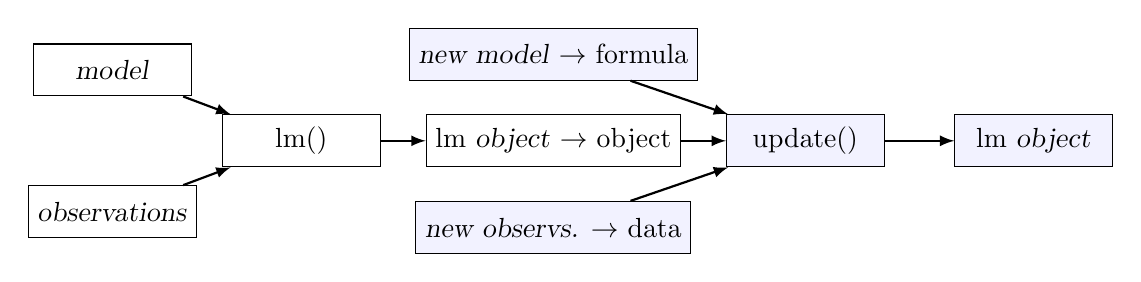
\begin{tikzpicture}[node distance=1.4cm, scale=0.5]
\node (model) [tprocess] {\textsl{model}};
\node (data) [tprocess, below of=model, yshift=-0.4cm] {\textsl{observations}};
\node (fitfun) [tprocess, right of=model, yshift=-0.9cm, xshift=1cm] {\code{lm()}};
\node (fm) [tprocess, color = black, right of=fitfun, xshift=1.8cm] {\code{lm} \textsl{object} $\to$ \code{object}};
\node (update) [tprocess, color = black, right of=fm, xshift = 1.8cm, fill=blue!5] {\code{update()}};
\node (newmodel) [tprocess, above of=fm, fill=blue!5, yshift=-0.3cm] {\textsl{new model} $\to$ \code{formula}};
\node (newdata) [tprocess, below of=fm, fill=blue!5, yshift=0.3cm] {\textsl{new observs.} $\to$ \code{data}};
\node (newfm) [tprocess, color = black, right of=update, xshift=1.5cm, fill=blue!5] {\code{lm} \textsl{object}};
\draw [arrow] (model) -- (fitfun);
\draw [arrow] (data) -- (fitfun);
\draw [arrow] (fitfun) -- (fm);
\draw [arrow] (fm) -- (update);
\draw [arrow] (newmodel) -- (update);
\draw [arrow] (newdata) -- (update);
\draw [arrow] (update) -- (newfm);
\end{tikzpicture}
\end{small}
\end{center}

\begin{infobox}
Model fit objects created with other functions from base \Rlang and extension packages usually also contain \code{data} and \code{call} members. In some cases the structure of the object is different, and not always all the accessor methods are available, but \Rlang's approach is followed by most extension packages.
\end{infobox}

\begin{explainbox}
Method \Rfunction{update()} retrieves the call from the model fit object, modifies it and, by default, evaluates it. It calls method \Rfunction{getCall()} to extract the call from the model fit object. The default \Rfunction{update()} method works as long as the model-fit object contains a member named \code{call} or a specialization of \Rfunction{getCall()} able to extract the call is available. Because of this, method \Rfunction{update()} can be used with models fitted with many different methods. Some packages define specializations of method \Rfunction{update()} that take advantage of previous estimates when evaluating the updated call.
\end{explainbox}

For the next example we recreate the model fit object \code{fm4} from page \pageref{chunk:stat:fm4}.

\begin{knitrout}\footnotesize
\definecolor{shadecolor}{rgb}{1, 1, 1}\color{fgcolor}\begin{kframe}
\begin{alltt}
\hlstd{fm4} \hlkwb{<-} \hlkwd{lm}\hlstd{(count} \hlopt{~} \hlstd{spray,} \hlkwc{data} \hlstd{= InsectSprays)}
\hlkwd{anova}\hlstd{(fm4)}
\end{alltt}
\begin{verbatim}
## Analysis of Variance Table
## 
## Response: count
##           Df Sum Sq Mean Sq F value    Pr(>F)    
## spray      5 2668.8  533.77  34.702 < 2.2e-16 ***
## Residuals 66 1015.2   15.38                      
## ---
## Signif. codes:  0 '***' 0.001 '**' 0.01 '*' 0.05 '.' 0.1 ' ' 1
\end{verbatim}
\begin{alltt}
\hlstd{fm4a} \hlkwb{<-} \hlkwd{update}\hlstd{(fm4,} \hlkwc{formula} \hlstd{=} \hlkwd{log10}\hlstd{(count} \hlopt{+} \hlnum{1}\hlstd{)} \hlopt{~} \hlstd{spray)}
\hlkwd{anova}\hlstd{(fm4a)}
\end{alltt}
\begin{verbatim}
## Analysis of Variance Table
## 
## Response: log10(count + 1)
##           Df Sum Sq Mean Sq F value    Pr(>F)    
## spray      5 7.2649 1.45297  46.007 < 2.2e-16 ***
## Residuals 66 2.0844 0.03158                      
## ---
## Signif. codes:  0 '***' 0.001 '**' 0.01 '*' 0.05 '.' 0.1 ' ' 1
\end{verbatim}
\end{kframe}
\end{knitrout}

\begin{playground}
Print \code{fm4\$call} and \code{fm4a\$call}. These two calls differ in the argument to \code{formula}. What other members have been updated in \code{fm4a} compared to \code{fm4}?
\end{playground}

In the chunk above we replaced the argument passed to \code{formula}. This is a frequent use, but for example to fit the same model to a subset of the data we can pass a suitable argument to parameter \code{subset}.

\begin{knitrout}\footnotesize
\definecolor{shadecolor}{rgb}{1, 1, 1}\color{fgcolor}\begin{kframe}
\begin{alltt}
\hlstd{fm4b} \hlkwb{<-} \hlkwd{update}\hlstd{(fm4,} \hlkwc{subset} \hlstd{=} \hlopt{!}\hlstd{spray} \hlopt \hlkwd{c}\hlstd{(}\hlstr{"A"}\hlstd{,} \hlstr{"B"}\hlstd{))}
\hlkwd{anova}\hlstd{(fm4b)}
\end{alltt}
\begin{verbatim}
## Analysis of Variance Table
## 
## Response: count
##           Df Sum Sq Mean Sq F value    Pr(>F)    
## spray      3 1608.4  536.14  41.422 7.119e-13 ***
## Residuals 44  569.5   12.94                      
## ---
## Signif. codes:  0 '***' 0.001 '**' 0.01 '*' 0.05 '.' 0.1 ' ' 1
\end{verbatim}
\end{kframe}
\end{knitrout}

\begin{advplayground}
When having many treatments with long names, which is not the case here, instead of listing the factor levels for which to subset the data, it can be convenient to use regular expressions for pattern matching. Please run the code below, and investigate why \code{anova(fm4b)} and \code{anova(fm4c)} produce the same ANOVA table printout, but the fit model objects are not identical. You can use \code{str()} to explore if any members differ between the two objects.

\begin{knitrout}\footnotesize
\definecolor{shadecolor}{rgb}{1, 1, 1}\color{fgcolor}\begin{kframe}
\begin{alltt}
\hlstd{fm4c} \hlkwb{<-} \hlkwd{update}\hlstd{(fm4,} \hlkwc{subset} \hlstd{=} \hlopt{!}\hlkwd{grepl}\hlstd{(}\hlstr{"[AB]"}\hlstd{, spray))}
\hlkwd{anova}\hlstd{(fm4c)}
\hlkwd{identical}\hlstd{(fm4b, fm4c)}
\end{alltt}
\end{kframe}
\end{knitrout}

\end{advplayground}

\begin{explainbox}
In the presence of multiple explanatory variables, or when using polynomial regression, using \Rfunction{update()} makes is easier to compare models with \Rfunction{anova()}.

Method \Rfunction{update()} is specially convenient when using model fitting functions with many formal parameters. It plays an additional role when fitting is done by numerical approximation, as the previously computed estimates are used as the starting values for the numerical calculations required for fitting the updated model.
\end{explainbox}

\begin{warningbox}
That the data are stored in the model fit object ensures that the use of methods like \Rfunction{update()} and various computations on the fit results can be reliably and consistently done irrespective of the presence or not of the same data in \Rlang's current-session. However, it should be kept in mind that changes to the original data done after the model fit object was created will not be reflected in the model fit objects returned by \Rfunction{update()} unless the new data are passed as an argument.
\end{warningbox}
\index{fitted models!updating|)}

\index{fitted models!stepwise selection|(}\index{linear models!stepwise regression|(}
Step-wise multiple regression, either in the \emph{forward} direction from simpler to more complex models, in the backward direction from more complex to simpler models or in both directions is implemented in base \Rlang's \emph{method} \Rfunction{step()} using Akaike's information criterion (AIC)\index{Akaike's An Information Criterion@Akaike's \emph{An Information Criterion}} as the selection criterion. Use of method \Rfunction{step()} from base \Rlang is possible with \code{lm()} and \code{glm} fits. AIC is described on page \pageref{par:stats:AIC}.

\begin{center}
\begin{small}
\begin{tikzpicture}[node distance=1.4cm, scale=0.5]
\node (model) [tprocess] {\textsl{model}};
\node (data) [tprocess, below of=model, yshift=-0.4cm] {\textsl{observations}};
\node (fitfun) [tprocess, right of=model, yshift=-0.9cm, xshift=1cm] {\code{lm()}};
\node (fm) [tprocess, color = black, right of=fitfun, xshift=1.8cm] {\code{lm} \textsl{object} $\to$ \code{object}};
\node (step) [tprocess, color = black, right of=fm, xshift = 1.8cm, fill=blue!5] {\code{step()}};
\node (newmodels) [tprocess, dashed, above of=fm, fill=blue!5, yshift=-0.3cm] {\textsl{new model(s)} $\to$ \code{scope}};
\node (newfm) [tprocess, color = black, right of=update, xshift=1.5cm, fill=blue!5] {\code{lm} \textsl{object}};
\draw [arrow] (model) -- (fitfun);
\draw [arrow] (data) -- (fitfun);
\draw [arrow] (fitfun) -- (fm);
\draw [arrow] (fm) -- (update);
\draw [arrow, dashed] (newmodels) -- (step);
\draw [arrow] (step) -- (newfm);
\end{tikzpicture}
\end{small}
\end{center}


For the next example we recreate the model fit object \code{fm3} from page \pageref{chunk:stats:fm3} for a polynomial regression. If as shown here, no models are passed through formal parameter \code{scope}, the previously fit model will be simplified, if possible. Method \Rfunction{step()} by default prints to the console a trace of the models tried and the corresponding AIC estimates.

\begin{knitrout}\footnotesize
\definecolor{shadecolor}{rgb}{1, 1, 1}\color{fgcolor}\begin{kframe}
\begin{alltt}
\hlstd{fm3} \hlkwb{<-} \hlkwd{lm}\hlstd{(dist} \hlopt{~} \hlstd{speed} \hlopt{+} \hlkwd{I}\hlstd{(speed}\hlopt{^}\hlnum{2}\hlstd{),} \hlkwc{data} \hlstd{= cars)}
\hlstd{fm3a} \hlkwb{<-} \hlkwd{step}\hlstd{(fm3)}
\end{alltt}
\begin{verbatim}
## Start:  AIC=274.88
## dist ~ speed + I(speed^2)
## 
##              Df Sum of Sq   RSS    AIC
## - speed       1     46.42 10871 273.09
## <none>                    10825 274.88
## - I(speed^2)  1    528.81 11354 275.26
## 
## Step:  AIC=273.09
## dist ~ I(speed^2)
## 
##              Df Sum of Sq   RSS    AIC
## <none>                    10871 273.09
## - I(speed^2)  1     21668 32539 325.91
\end{verbatim}
\end{kframe}
\end{knitrout}

We use \Rfunction{summary()} on both the original and updated models.

\begin{knitrout}\footnotesize
\definecolor{shadecolor}{rgb}{1, 1, 1}\color{fgcolor}\begin{kframe}
\begin{alltt}
\hlkwd{summary}\hlstd{(fm3)}
\end{alltt}
\begin{verbatim}
## 
## Call:
## lm(formula = dist ~ speed + I(speed^2), data = cars)
## 
## Residuals:
##     Min      1Q  Median      3Q     Max 
## -28.720  -9.184  -3.188   4.628  45.152 
## 
## Coefficients:
##             Estimate Std. Error t value Pr(>|t|)
## (Intercept)  2.47014   14.81716   0.167    0.868
## speed        0.91329    2.03422   0.449    0.656
## I(speed^2)   0.09996    0.06597   1.515    0.136
## 
## Residual standard error: 15.18 on 47 degrees of freedom
## Multiple R-squared:  0.6673,	Adjusted R-squared:  0.6532 
## F-statistic: 47.14 on 2 and 47 DF,  p-value: 5.852e-12
\end{verbatim}
\begin{alltt}
\hlkwd{summary}\hlstd{(fm3a)}
\end{alltt}
\begin{verbatim}
## 
## Call:
## lm(formula = dist ~ I(speed^2), data = cars)
## 
## Residuals:
##     Min      1Q  Median      3Q     Max 
## -28.448  -9.211  -3.594   5.076  45.862 
## 
## Coefficients:
##             Estimate Std. Error t value Pr(>|t|)    
## (Intercept)  8.86005    4.08633   2.168   0.0351 *  
## I(speed^2)   0.12897    0.01319   9.781  5.2e-13 ***
## ---
## Signif. codes:  0 '***' 0.001 '**' 0.01 '*' 0.05 '.' 0.1 ' ' 1
## 
## Residual standard error: 15.05 on 48 degrees of freedom
## Multiple R-squared:  0.6659,	Adjusted R-squared:  0.6589 
## F-statistic: 95.67 on 1 and 48 DF,  p-value: 5.2e-13
\end{verbatim}
\end{kframe}
\end{knitrout}

If we pass a single model with additional terms through parameter \code{scope} this will be taken as the most complex model to be assessed. If, instead of one model, we pass two nested models in a list and name them \code{lower} and \code{upper}, they will delimit the scope of the stepwise search. In the next example we see that first a backward search is done and term \code{speed} is removed as removal decreases AIC. Subsequently a forward search is done unsuccessfully for a model with smaller AIC.

\begin{knitrout}\footnotesize
\definecolor{shadecolor}{rgb}{1, 1, 1}\color{fgcolor}\begin{kframe}
\begin{alltt}
\hlstd{fm3b} \hlkwb{<-}
  \hlkwd{step}\hlstd{(fm3,}
       \hlkwc{scope} \hlstd{= dist} \hlopt{~} \hlstd{speed} \hlopt{+} \hlkwd{I}\hlstd{(speed}\hlopt{^}\hlnum{2}\hlstd{)} \hlopt{+} \hlkwd{I}\hlstd{(speed}\hlopt{^}\hlnum{3}\hlstd{)} \hlopt{+} \hlkwd{I}\hlstd{(speed}\hlopt{^}\hlnum{4}\hlstd{))}
\end{alltt}
\begin{verbatim}
## Start:  AIC=274.88
## dist ~ speed + I(speed^2)
## 
##              Df Sum of Sq   RSS    AIC
## - speed       1     46.42 10871 273.09
## <none>                    10825 274.88
## - I(speed^2)  1    528.81 11354 275.26
## + I(speed^4)  1    233.62 10591 275.79
## + I(speed^3)  1    190.35 10634 275.99
## 
## Step:  AIC=273.09
## dist ~ I(speed^2)
## 
##              Df Sum of Sq   RSS    AIC
## <none>                    10871 273.09
## + speed       1      46.4 10825 274.88
## + I(speed^3)  1       5.6 10866 275.07
## + I(speed^4)  1       0.0 10871 275.09
## - I(speed^2)  1   21667.8 32539 325.91
\end{verbatim}
\begin{alltt}
\hlkwd{summary}\hlstd{(fm3b)}
\end{alltt}
\begin{verbatim}
## 
## Call:
## lm(formula = dist ~ I(speed^2), data = cars)
## 
## Residuals:
##     Min      1Q  Median      3Q     Max 
## -28.448  -9.211  -3.594   5.076  45.862 
## 
## Coefficients:
##             Estimate Std. Error t value Pr(>|t|)    
## (Intercept)  8.86005    4.08633   2.168   0.0351 *  
## I(speed^2)   0.12897    0.01319   9.781  5.2e-13 ***
## ---
## Signif. codes:  0 '***' 0.001 '**' 0.01 '*' 0.05 '.' 0.1 ' ' 1
## 
## Residual standard error: 15.05 on 48 degrees of freedom
## Multiple R-squared:  0.6659,	Adjusted R-squared:  0.6589 
## F-statistic: 95.67 on 1 and 48 DF,  p-value: 5.2e-13
\end{verbatim}
\end{kframe}
\end{knitrout}

\begin{playground}
Explain why the stepwise model selection in the code below differs from those in the two previous examples. Consult \code{help(step)} is necessary.

\begin{knitrout}\footnotesize
\definecolor{shadecolor}{rgb}{1, 1, 1}\color{fgcolor}\begin{kframe}
\begin{alltt}
\hlstd{fm3c} \hlkwb{<-}
  \hlkwd{step}\hlstd{(fm3,}
       \hlkwc{scope} \hlstd{=} \hlkwd{list}\hlstd{(}\hlkwc{lower} \hlstd{= dist} \hlopt{~} \hlstd{speed,}
                    \hlkwc{upper} \hlstd{= dist} \hlopt{~} \hlstd{speed} \hlopt{+} \hlkwd{I}\hlstd{(speed}\hlopt{^}\hlnum{2}\hlstd{)} \hlopt{+} \hlkwd{I}\hlstd{(speed}\hlopt{^}\hlnum{3}\hlstd{)} \hlopt{+} \hlkwd{I}\hlstd{(speed}\hlopt{^}\hlnum{4}\hlstd{)))}
\hlkwd{summary}\hlstd{(fm3c)}
\end{alltt}
\end{kframe}
\end{knitrout}

\end{playground}

Functions \Rfunction{update()} and \Rfunction{step()} are \emph{convenience functions} as they provide direct and/or simpler access to operations available through other functions or combined use of multiple functions.
\index{linear models!stepwise regression|)}\index{fitted models!stepwise selection|)}

\section{Generalized linear models}\label{sec:stat:GLM}
\index{generalized linear models|(}\index{models!generalized linear|see{generalized linear models}}
\index{GLM|see{generalized linear models}}

Linear models make the assumption of normally distributed residuals. Generalized linear models, fitted with function \Rfunction{glm()} are more flexible, and allow the assumed distribution to be selected as well as the link function.

\begin{center}
\begin{small}
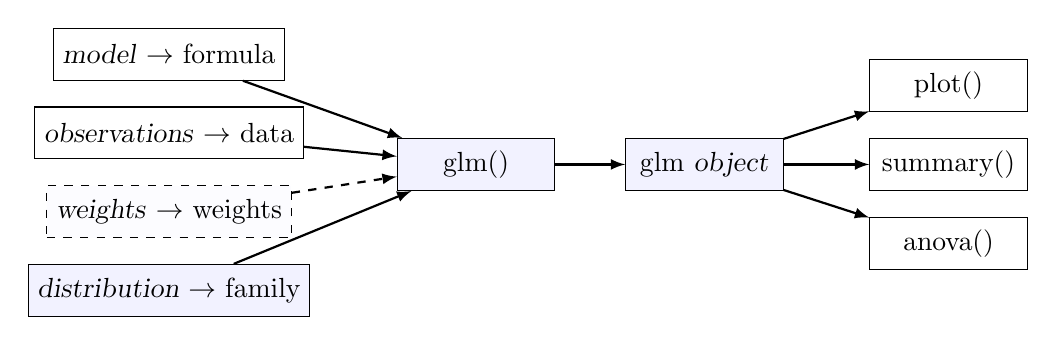
\begin{tikzpicture}[node distance=1.4cm, scale=0.5]
\node (model) [tprocess] {\textsl{model} $\to$ \code{formula}};
\node (data) [tprocess, below of=model, yshift = 0.4cm] {\textsl{observations} $\to$ \code{data}};
\node (weights) [tprocess, dashed, below of=data, fill=blue!1, yshift = 0.4cm] {\textsl{weights} $\to$ \code{weights}};
\node (family) [tprocess, below of=weights, fill=blue!5, yshift = 0.4cm] {\textsl{distribution} $\to$ \code{family}};
\node (fitfun) [tprocess, right of=data, xshift=2.5cm, yshift = -0.4cm,fill=blue!5] {\code{glm()}};
\node (fm) [tprocess, color = black, right of=fitfun, xshift=1.5cm, fill=blue!5] {\code{glm} \textsl{object}};
\node (summary) [tprocess, color = black, right of=fm, xshift=1.7cm] {\code{summary()}};
\node (anova) [tprocess, color = black, below of=summary, yshift = 0.4cm] {\code{anova()}};
\node (plot) [tprocess, color = black, above of=summary, yshift = -0.4cm] {\code{plot()}};
\draw [arrow] (model) -- (fitfun);
\draw [arrow] (data) -- (fitfun);
\draw [arrow, dashed] (weights) -- (fitfun);
\draw [arrow] (family) -- (fitfun);
\draw [arrow] (fitfun) -- (fm);
\draw [arrow] (fm) -- (plot);
\draw [arrow] (fm) -- (anova);
\draw [arrow] (fm) -- (summary);
\end{tikzpicture}
\end{small}
\end{center}

For the analysis of the \Rdata{InsectSprays} data set above (section \ref{sec:anova} on page \pageref{sec:anova}), the Normal distribution is not a good approximation as count data deviates from it. This was visible in the quantile--quantile plot above.

For count data, GLMs provide a better alternative. In the example below we fit the same model as above, but we assume a quasi-Poisson distribution instead of the Normal. In addition to the model formula we need to pass an argument through \code{family} giving the error distribution to be assumed---the default for \code{family} is \code{gaussian} or Normal distribution.

\begin{knitrout}\footnotesize
\definecolor{shadecolor}{rgb}{1, 1, 1}\color{fgcolor}\begin{kframe}
\begin{alltt}
\hlstd{fm10} \hlkwb{<-} \hlkwd{glm}\hlstd{(count} \hlopt{~} \hlstd{spray,} \hlkwc{data} \hlstd{= InsectSprays,} \hlkwc{family} \hlstd{= quasipoisson)}
\hlkwd{anova}\hlstd{(fm10)}
\end{alltt}
\begin{verbatim}
## Analysis of Deviance Table
## 
## Model: quasipoisson, link: log
## 
## Response: count
## 
## Terms added sequentially (first to last)
## 
## 
##       Df Deviance Resid. Df Resid. Dev
## NULL                     71     409.04
## spray  5   310.71        66      98.33
\end{verbatim}
\end{kframe}
\end{knitrout}

The printout from the \Rfunction{anova()} method for GLM fits has some differences to that for LM fits. By default, no significance test is computed, as a knowledgeable choice is required depending on the characteristics of the model and data. We here use \code{"F"} as an argument to request an $F$-test.

\begin{knitrout}\footnotesize
\definecolor{shadecolor}{rgb}{1, 1, 1}\color{fgcolor}\begin{kframe}
\begin{alltt}
\hlkwd{anova}\hlstd{(fm10,} \hlkwc{test} \hlstd{=} \hlstr{"F"}\hlstd{)}
\end{alltt}
\begin{verbatim}
## Analysis of Deviance Table
## 
## Model: quasipoisson, link: log
## 
## Response: count
## 
## Terms added sequentially (first to last)
## 
## 
##       Df Deviance Resid. Df Resid. Dev      F    Pr(>F)    
## NULL                     71     409.04                     
## spray  5   310.71        66      98.33 41.216 < 2.2e-16 ***
## ---
## Signif. codes:  0 '***' 0.001 '**' 0.01 '*' 0.05 '.' 0.1 ' ' 1
\end{verbatim}
\end{kframe}
\end{knitrout}

Method \Rfunction{plot()} as for linear-model fits, produces diagnosis plots. We show as above the q-q-plot of residuals.

\begin{knitrout}\footnotesize
\definecolor{shadecolor}{rgb}{1, 1, 1}\color{fgcolor}\begin{kframe}
\begin{alltt}
\hlkwd{plot}\hlstd{(fm10,} \hlkwc{which} \hlstd{=} \hlnum{3}\hlstd{)}
\end{alltt}
\end{kframe}

{\centering \includegraphics[width=.54\textwidth]{figure/pos-model-11-1} 

}


\end{knitrout}

We can extract different components similarly as described for linear models (see section \ref{sec:stat:LM} on page \pageref{sec:stat:LM}).

\begin{knitrout}\footnotesize
\definecolor{shadecolor}{rgb}{1, 1, 1}\color{fgcolor}\begin{kframe}
\begin{alltt}
\hlkwd{class}\hlstd{(fm10)}
\end{alltt}
\begin{verbatim}
## [1] "glm" "lm"
\end{verbatim}
\begin{alltt}
\hlkwd{summary}\hlstd{(fm10)}
\end{alltt}
\begin{verbatim}
## 
## Call:
## glm(formula = count ~ spray, family = quasipoisson, data = InsectSprays)
## 
## Coefficients:
##             Estimate Std. Error t value Pr(>|t|)    
## (Intercept)  2.67415    0.09309  28.728  < 2e-16 ***
## sprayB       0.05588    0.12984   0.430    0.668    
## sprayC      -1.94018    0.26263  -7.388 3.30e-10 ***
## sprayD      -1.08152    0.18499  -5.847 1.70e-07 ***
## sprayE      -1.42139    0.21110  -6.733 4.82e-09 ***
## sprayF       0.13926    0.12729   1.094    0.278    
## ---
## Signif. codes:  0 '***' 0.001 '**' 0.01 '*' 0.05 '.' 0.1 ' ' 1
## 
## (Dispersion parameter for quasipoisson family taken to be 1.507713)
## 
##     Null deviance: 409.041  on 71  degrees of freedom
## Residual deviance:  98.329  on 66  degrees of freedom
## AIC: NA
## 
## Number of Fisher Scoring iterations: 5
\end{verbatim}
\begin{alltt}
\hlkwd{head}\hlstd{(}\hlkwd{residuals}\hlstd{(fm10))}
\end{alltt}
\begin{verbatim}
##          1          2          3          4          5          6 
## -1.2524891 -2.1919537  1.3650439 -0.1320721 -0.1320721 -0.6768988
\end{verbatim}
\begin{alltt}
\hlkwd{head}\hlstd{(}\hlkwd{fitted}\hlstd{(fm10))}
\end{alltt}
\begin{verbatim}
##    1    2    3    4    5    6 
## 14.5 14.5 14.5 14.5 14.5 14.5
\end{verbatim}
\end{kframe}
\end{knitrout}

\begin{explainbox}
If we use \code{str()} or \code{names()} we can see that there are some differences with respect to linear model fits. The returned object is of a different class and contains some members not present in linear models. Two of these have to do with the iterative approximation method used, \code{iter} contains the number of iterations used  and \code{converged} the success or not in finding a solution.

\begin{knitrout}\footnotesize
\definecolor{shadecolor}{rgb}{1, 1, 1}\color{fgcolor}\begin{kframe}
\begin{alltt}
\hlkwd{names}\hlstd{(fm10)}
\end{alltt}
\begin{verbatim}
##  [1] "coefficients"      "residuals"         "fitted.values"    
##  [4] "effects"           "R"                 "rank"             
##  [7] "qr"                "family"            "linear.predictors"
## [10] "deviance"          "aic"               "null.deviance"    
## [13] "iter"              "weights"           "prior.weights"    
## [16] "df.residual"       "df.null"           "y"                
## [19] "converged"         "boundary"          "model"            
## [22] "call"              "formula"           "terms"            
## [25] "data"              "offset"            "control"          
## [28] "method"            "contrasts"         "xlevels"
\end{verbatim}
\begin{alltt}
\hlstd{fm10}\hlopt{$}\hlstd{converged}
\end{alltt}
\begin{verbatim}
## [1] TRUE
\end{verbatim}
\begin{alltt}
\hlstd{fm10}\hlopt{$}\hlstd{iter}
\end{alltt}
\begin{verbatim}
## [1] 5
\end{verbatim}
\end{kframe}
\end{knitrout}
\end{explainbox}

Methods \code{update()} and \code{step()}, described for \code{lm()} in section \ref{sec:stat:update:step} on page \pageref{sec:stat:update:step}, can be also used with models fitted with \code{glm()}.

\index{generalized linear models|)}

\section{Non-linear regression}\label{sec:stat:NLS}
\index{non-linear models|(}%
\index{models!non-linear|see{non-linear models}}%
\index{NLS|see{non-linear models}}

Function \Rfunction{nls()} is \Rlang's workhorse for fitting non-linear models. By \emph{non-linear} it is meant non-linear \emph{in the parameters} whose values are being estimated through fitting the model to data. This is different from the shape of the function when plotted---i.e., polynomials of any degree are linear models. In contrast, the Michaelis-Menten equation used in chemistry and the Gompertz equation used to describe growth are non-linear models in their parameters.

While analytical algorithms exist for finding estimates for the parameters of linear models, in the case of non-linear models, the estimates are obtained by approximation. For analytical solutions, estimates can always be obtained, except in infrequent pathological cases where reliance on floating point numbers with limited resolution introduces rounding errors that ``break'' mathematical algorithms that are valid for real numbers. For approximations obtained through iteration, cases when the algorithm fails to \emph{converge} onto an answer are relatively common. Iterative algorithms attempt to improve an initial guess for the values of the parameters to be estimated, a guess frequently supplied by the user. In each iteration the estimate obtained in the previous iteration is used as the starting value, and this process is repeated one time after another. The expectation is that after a finite number of iterations the algorithm will converge into a solution that ``cannot'' be improved further. In real life we stop iteration when the improvement in the fit is smaller than a certain threshold, or when no convergence has been achieved after a certain maximum number of iterations. In the first case, we usually obtain good estimates; in the second case, we do not obtain usable estimates and need to look for different ways of obtaining them. When convergence fails, the first thing to do is to try different starting values and if this also fails, switch to a different computational algorithm. These steps usually help, but not always. Good starting values are in many cases crucial and in some cases ``guesses'' can be obtained using either graphical or analytical approximations.

\begin{center}
\begin{small}
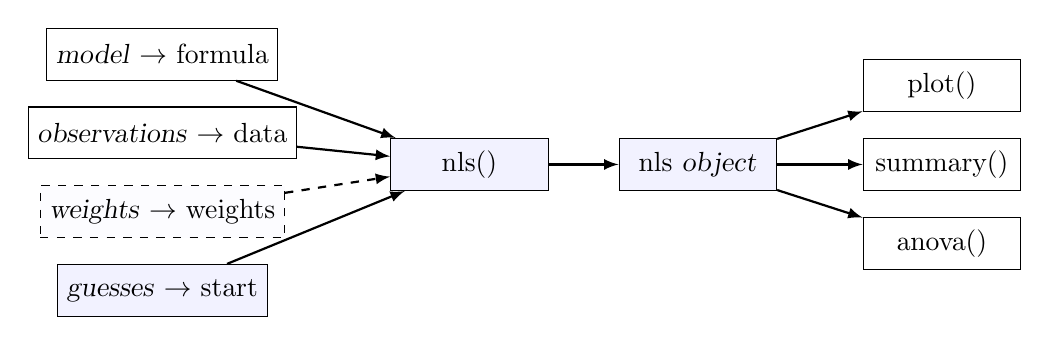
\begin{tikzpicture}[node distance=1.4cm, scale=0.5]
\node (model) [tprocess] {\textsl{model} $\to$ \code{formula}};
\node (data) [tprocess, below of=model, yshift = 0.4cm] {\textsl{observations} $\to$ \code{data}};
\node (weights) [tprocess, dashed, below of=data, yshift = 0.4cm, fill=blue!1] {\textsl{weights} $\to$ \code{weights}};
\node (guess) [tprocess, below of=weights, fill=blue!5, yshift = 0.4cm] {\textsl{guesses} $\to$ \code{start}};
\node (fitfun) [tprocess, right of=data, xshift=2.5cm, yshift = -0.4cm, fill=blue!5] {\code{nls()}};
\node (fm) [tprocess, color = black, right of=fitfun, xshift=1.5cm, fill=blue!5] {\code{nls} \textsl{object}};
\node (summary) [tprocess, color = black, right of=fm, xshift=1.7cm] {\code{summary()}};
\node (anova) [tprocess, color = black, below of=summary, yshift = 0.4cm] {\code{anova()}};
\node (plot) [tprocess, color = black, above of=summary, yshift = -0.4cm] {\code{plot()}};
\draw [arrow] (model) -- (fitfun);
\draw [arrow] (data) -- (fitfun);
\draw [arrow, dashed] (weights) -- (fitfun);
\draw [arrow] (guess) -- (fitfun);
\draw [arrow] (fitfun) -- (fm);
\draw [arrow] (fm) -- (plot);
\draw [arrow] (fm) -- (anova);
\draw [arrow] (fm) -- (summary);
\end{tikzpicture}
\end{small}
\end{center}

For functions for which computational algorithms exist for ``guessing'' suitable starting values, \Rlang provides a mechanism for packaging the function to be fitted together with the function generating the starting values. These functions go by the name of \emph{self-starting functions} and relieve the user from the burden of guessing and supplying suitable starting values. The\index{self-starting functions} self-starting functions available in \Rlang are \code{SSasymp()}, \code{SSasympOff()}, \code{SSasympOrig()}, \code{SSbiexp()}, \code{SSfol()}, \code{SSfpl()}, \code{SSgompertz()}, \code{SSlogis()}, \code{SSmicmen()}, and \code{SSweibull()}. Function \code{selfStart()} can be used to define new ones. All these functions can be used when fitting models with \Rfunction{nls} or \Rfunction{nlme}. Please, check the respective help pages for details.

In the case of \Rfunction{nls()} the specification of the model to be fitted differs from that used for linear models. We will use as an example fitting the Michaelis-Menten equation\index{Michaelis-Menten equation} describing reaction kinetics\index{chemical reaction kinetics} in biochemistry and chemistry. The mathematical formulation is given by:

\begin{equation}\label{eq:michaelis:menten}
v = \frac{\mathrm{d} [P]}{\mathrm{d} t} = \frac{V_{\mathrm{max}} [S]}{K_{\mathrm{M}} + [S]}
\end{equation}

The function takes its name from Michaelis and Menten's paper from 1913 \autocite{Johnson2011}. A self-starting function implementing the Michaelis-Menten equation is available in \Rlang under the name \Rfunction{SSmicmen()}\index{models!selfstart@{\texttt{selfStart}}}. We will use the \Rdata{Puromycin} data set.

\begin{knitrout}\footnotesize
\definecolor{shadecolor}{rgb}{1, 1, 1}\color{fgcolor}\begin{kframe}
\begin{alltt}
\hlkwd{data}\hlstd{(Puromycin)}
\hlkwd{names}\hlstd{(Puromycin)}
\end{alltt}
\begin{verbatim}
## [1] "conc"  "rate"  "state"
\end{verbatim}
\end{kframe}
\end{knitrout}

\begin{knitrout}\footnotesize
\definecolor{shadecolor}{rgb}{1, 1, 1}\color{fgcolor}\begin{kframe}
\begin{alltt}
\hlstd{fm21} \hlkwb{<-} \hlkwd{nls}\hlstd{(rate} \hlopt{~} \hlkwd{SSmicmen}\hlstd{(conc, Vm, K),} \hlkwc{data} \hlstd{= Puromycin,}
            \hlkwc{subset} \hlstd{= state} \hlopt{==} \hlstr{"treated"}\hlstd{)}
\end{alltt}
\end{kframe}
\end{knitrout}

We can extract different components similarly as described for linear models (see section \ref{sec:stat:LM} on page \pageref{sec:stat:LM}).

\begin{knitrout}\footnotesize
\definecolor{shadecolor}{rgb}{1, 1, 1}\color{fgcolor}\begin{kframe}
\begin{alltt}
\hlkwd{class}\hlstd{(fm21)}
\end{alltt}
\begin{verbatim}
## [1] "nls"
\end{verbatim}
\begin{alltt}
\hlkwd{summary}\hlstd{(fm21)}
\end{alltt}
\begin{verbatim}
## 
## Formula: rate ~ SSmicmen(conc, Vm, K)
## 
## Parameters:
##     Estimate Std. Error t value Pr(>|t|)    
## Vm 2.127e+02  6.947e+00  30.615 3.24e-11 ***
## K  6.412e-02  8.281e-03   7.743 1.57e-05 ***
## ---
## Signif. codes:  0 '***' 0.001 '**' 0.01 '*' 0.05 '.' 0.1 ' ' 1
## 
## Residual standard error: 10.93 on 10 degrees of freedom
## 
## Number of iterations to convergence: 0 
## Achieved convergence tolerance: 1.929e-06
\end{verbatim}
\begin{alltt}
\hlkwd{residuals}\hlstd{(fm21)}
\end{alltt}
\begin{verbatim}
##  [1]  25.4339971  -3.5660029  -5.8109605   4.1890395 -11.3616075   4.6383925
##  [7]  -5.6846886 -12.6846886   0.1670798  10.1670798   6.0311723  -0.9688277
## attr(,"label")
## [1] "Residuals"
\end{verbatim}
\begin{alltt}
\hlkwd{fitted}\hlstd{(fm21)}
\end{alltt}
\begin{verbatim}
##  [1]  50.5660  50.5660 102.8110 102.8110 134.3616 134.3616 164.6847 164.6847
##  [9] 190.8329 190.8329 200.9688 200.9688
## attr(,"label")
## [1] "Fitted values"
\end{verbatim}
\end{kframe}
\end{knitrout}

\begin{explainbox}
If we use \code{str()} or \code{names()} we can see that there are differences with respect to linear model and generalized model fits. The returned object is of class \code{nls} and contains some new members and lacks others. Two members are related to the iterative approximation method used, \code{control} containing nested members holding iteration settings, and \code{convInfo} (convergence information) with nested members with information on the outcome of the iterative algorithm.

\begin{knitrout}\footnotesize
\definecolor{shadecolor}{rgb}{1, 1, 1}\color{fgcolor}\begin{kframe}
\begin{alltt}
\hlkwd{str}\hlstd{(fm21,} \hlkwc{max.level} \hlstd{=} \hlnum{1}\hlstd{)}
\end{alltt}
\begin{verbatim}
## List of 6
##  $ m          :List of 16
##   ..- attr(*, "class")= chr "nlsModel"
##  $ convInfo   :List of 5
##  $ data       : symbol Puromycin
##  $ call       : language nls(formula = rate ~ SSmicmen(conc, Vm, K), data = Puromycin, subset = state ==      "treated", algorithm = "defa| __truncated__ ...
##  $ dataClasses: Named chr "numeric"
##   ..- attr(*, "names")= chr "conc"
##  $ control    :List of 7
##  - attr(*, "class")= chr "nls"
\end{verbatim}
\end{kframe}
\end{knitrout}

\begin{knitrout}\footnotesize
\definecolor{shadecolor}{rgb}{1, 1, 1}\color{fgcolor}\begin{kframe}
\begin{alltt}
\hlstd{fm21}\hlopt{$}\hlstd{convInfo}
\end{alltt}
\begin{verbatim}
## $isConv
## [1] TRUE
## 
## $finIter
## [1] 0
## 
## $finTol
## [1] 1.928554e-06
## 
## $stopCode
## [1] 0
## 
## $stopMessage
## [1] "converged"
\end{verbatim}
\end{kframe}
\end{knitrout}
\end{explainbox}

Method \code{update()}, described for \code{lm()} in section \ref{sec:stat:update:step} on page \pageref{sec:stat:update:step}, can be also used with models fitted with \code{glm()}.

\index{non-linear models|)}

\section{Splines and local regression}\label{sec:stat:splines}

The name ``spline´´ derives from the tool used by draftsmen to draw smooth curves. Originally, a spline of soft wood was used as a flexible guide to draw arbitrary curves. Later the wood splines were replaced by a rod of flexible metal, such as lead, encased in plastic or similar material but the original name persisted. In mathematics, splines are functions that describe smooth and flexible curves.

Most of the model fits given above as examples produce estimates for parameters that are interpretable in the real world, directly in the case of mechanistic models like the estimate of reaction constants or at least indicating broadly a relationship between two variables as in the case of linear regression. In the case of polynomials of degrees more than 2, parameter estimates no longer directly describe features of the data.

Splines take this a step farther and parameter estimates have no practical interest and the interest resides in the overall shape and position of the predicted curve. Splines consist in knots (or connection points) joined by straight or curved fitted lines, i.e., they are functions that are \emph{piecewise}. The simplest splines, are piece-wise linear, given by chained straight line segments connecting knots. In more complex splines the segments are polynomials, frequently cubic polynomials, that fulfil certain constraints at the knots. For example, that the slope or first derivative is the same for the two connected curve ``pieces'' at the knot where they are connected. This constraint ensures that the curve is smooth. In some cases similar constraints are imposed on higher order derivatives, for example to the second derivative to ensure that the curve of the first derivative is also smooth at the knots.

Splines are used in free-hand drawing with computers to draw arbitrary smooth curves. They are also be used for interpolation, in which case observations, assumed to be error-free, become the knots of a spline used to approximate intermediate values. Finally, splines can be used as models to be fit to observations subject to random variation. In this case splines fulfil the role of smoothers, as a curve that broadly describes a relationship among variables.

Splines are frequently used as smooth curves in plots as described in section \ref{sec:plot:smoothers} on page \pageref{sec:plot:smoothers}. Function \Rfunction{spline()} is used for interpolation and function \Rfunction{smooth.spline()} for smoothing by fitting a cubic spline (a spline where the knots are connected by third degree polynomials). Function \Rfunction{smooth.spline()} has a different user interface than that we used for model fit functions described above, as it only accepts \code{numeric} vectors as arguments to parameters \code{x} and \code{y}. Additional parameters make it possible to override the defaults for number of knots and adjust the stiffness or tendency towards a straight line. The \code{plot()} method differently to other fit functions produces a plot of the prediction.

\begin{center}
\begin{small}
\begin{tikzpicture}[node distance=1.4cm, scale=0.5]
\node (x) [tprocess, fill=blue!5] {\textsl{obs.} $\to$ \code{x}};
\node (y) [tprocess, below of=model, fill=blue!5] {\textsl{obs.} $\to$ \code{y}};
\node (fitfun) [tprocess, right of=model, yshift=-0.7cm, xshift=2cm, fill=blue!5] {\code{smooth.spline()}};
\node (fm) [tprocess, color = black, right of=fitfun, xshift=2.3cm, fill=blue!5] {\code{smooth.spline} \textsl{obj.}};
\node (pred) [tprocess, color = black, right of=fm, xshift=2.3cm] {\code{predict()}};
\node (fitted) [tprocess, color = black, above of=pred, yshift = -0.4cm] {\code{fitted()}};
\node (resid) [tprocess, color = black, below of=pred, yshift = +0.4cm] {\code{residuals()}};
\draw [arrow] (x) -- (fitfun);
\draw [arrow] (y) -- (fitfun);
\draw [arrow] (fitfun) -- (fm);
\draw [arrow] (fm) -- (pred);
\draw [arrow] (fm) -- (fitted);
\draw [arrow] (fm) -- (resid);
\end{tikzpicture}
\end{small}
\end{center}

\begin{knitrout}\footnotesize
\definecolor{shadecolor}{rgb}{1, 1, 1}\color{fgcolor}\begin{kframe}
\begin{alltt}
\hlstd{fs1} \hlkwb{<-} \hlkwd{smooth.spline}\hlstd{(}\hlkwc{x} \hlstd{= cars}\hlopt{$}\hlstd{speed,} \hlkwc{y} \hlstd{= cars}\hlopt{$}\hlstd{dist)}
\hlkwd{print}\hlstd{(fs1)}
\end{alltt}
\begin{verbatim}
## Call:
## smooth.spline(x = cars$speed, y = cars$dist)
## 
## Smoothing Parameter  spar= 0.7801305  lambda= 0.1112206 (11 iterations)
## Equivalent Degrees of Freedom (Df): 2.635278
## Penalized Criterion (RSS): 4187.776
## GCV: 244.1044
\end{verbatim}
\begin{alltt}
\hlkwd{plot}\hlstd{(fs1,} \hlkwc{type} \hlstd{=} \hlstr{"l"}\hlstd{)}
\hlkwd{points}\hlstd{(}\hlkwc{x} \hlstd{= cars}\hlopt{$}\hlstd{speed,} \hlkwc{y} \hlstd{= cars}\hlopt{$}\hlstd{dist)}
\end{alltt}
\end{kframe}

{\centering \includegraphics[width=.54\textwidth]{figure/pos-spline-01-1} 

}


\end{knitrout}

Function \Rfunction{loess} fits a polynomial surface using local fitting. Its user interface is rather similar to that of \code{glm()} with \code{formula}, \code{family} and \code{data} formal parameters. Additional parameters control ``stiffness'' or the extent of the local data used for fitting. The type of fit local or not used for individual explanatory variables can be controlled through parameter \code{parametric}.

\begin{center}
\begin{small}
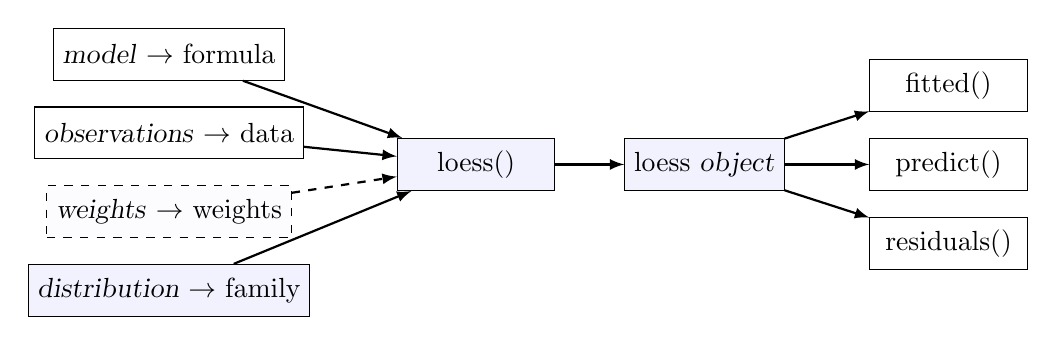
\begin{tikzpicture}[node distance=1.4cm, scale=0.5]
\node (model) [tprocess] {\textsl{model} $\to$ \code{formula}};
\node (data) [tprocess, below of=model, yshift = 0.4cm] {\textsl{observations} $\to$ \code{data}};
\node (weights) [tprocess, dashed, below of=data, fill=blue!1, yshift = 0.4cm] {\textsl{weights} $\to$ \code{weights}};
\node (family) [tprocess, below of=weights, fill=blue!5, yshift = 0.4cm] {\textsl{distribution} $\to$ \code{family}};
\node (fitfun) [tprocess, right of=data, xshift=2.5cm, yshift = -0.4cm, fill=blue!5] {\code{loess()}};
\node (fm) [tprocess, color = black, right of=fitfun, xshift=1.5cm, fill=blue!5] {\code{loess} \textsl{object}};
\node (pred) [tprocess, color = black, right of=fm, xshift=1.7cm] {\code{predict()}};
\node (fitted) [tprocess, color = black, above of=pred, yshift = -0.4cm] {\code{fitted()}};
\node (resid) [tprocess, color = black, below of=pred, yshift = +0.4cm] {\code{residuals()}};
\draw [arrow] (model) -- (fitfun);
\draw [arrow] (data) -- (fitfun);
\draw [arrow, dashed] (weights) -- (fitfun);
\draw [arrow] (family) -- (fitfun);
\draw [arrow] (fitfun) -- (fm);
\draw [arrow] (fm) -- (pred);
\draw [arrow] (fm) -- (fitted);
\draw [arrow] (fm) -- (resid);
\end{tikzpicture}
\end{small}
\end{center}

\begin{knitrout}\footnotesize
\definecolor{shadecolor}{rgb}{1, 1, 1}\color{fgcolor}\begin{kframe}
\begin{alltt}
\hlstd{floc} \hlkwb{<-} \hlkwd{loess}\hlstd{(dist} \hlopt{~} \hlstd{speed,} \hlkwc{data} \hlstd{= cars)}
\hlkwd{print}\hlstd{(floc)}
\end{alltt}
\begin{verbatim}
## Call:
## loess(formula = dist ~ speed, data = cars)
## 
## Number of Observations: 50 
## Equivalent Number of Parameters: 4.78 
## Residual Standard Error: 15.29
\end{verbatim}
\end{kframe}
\end{knitrout}

\begin{explainbox}
  Several modern approaches to data analysis, which do provide estimates of effects' significance and sizes, are based on the use of splines to describe the responses and even variance. Among them are additive models such as GAM and related methods \autocite[see][]{Wood2017} and functional data analysis (FDA) \autocite{Ramsay2009}. These methods are outside the scope of this book and implemented in specialized extension packages.
\end{explainbox}

\section{Model formulas}\label{sec:stat:formulas}
\index{model formulas|(}
Model formulas, such as \code{y ~ x} are widely used in \Rlang, both in model fitting as exemplified in previous sections of this chapter and in plotting when using base \Rlang \Rmethod{plot()} methods.

\Rlang is consistent and flexible in how it treats various objects, to a extent that can be surprising to those familiar with other computer languages. Model formulas are objects of class \Rclass{formula} and mode \Rclass{call} and can be manipulated and stored similarly to objects of other classes.

\begin{knitrout}\footnotesize
\definecolor{shadecolor}{rgb}{1, 1, 1}\color{fgcolor}\begin{kframe}
\begin{alltt}
\hlkwd{class}\hlstd{(y} \hlopt{~} \hlstd{x)}
\end{alltt}
\begin{verbatim}
## [1] "formula"
\end{verbatim}
\begin{alltt}
\hlkwd{mode}\hlstd{(y} \hlopt{~} \hlstd{x)}
\end{alltt}
\begin{verbatim}
## [1] "call"
\end{verbatim}
\end{kframe}
\end{knitrout}

Like any other \Rlang object formulas can be assigned to variables and be members of lists and vectors. Consequently, the first linear model fit example from page \pageref{chunk:lm:models1} can be rewritten as follows.

\begin{knitrout}\footnotesize
\definecolor{shadecolor}{rgb}{1, 1, 1}\color{fgcolor}\begin{kframe}
\begin{alltt}
\hlstd{my.formula} \hlkwb{<-} \hlstd{dist} \hlopt{~} \hlnum{1} \hlopt{+} \hlstd{speed}
\hlstd{fm1} \hlkwb{<-} \hlkwd{lm}\hlstd{(my.formula,} \hlkwc{data}\hlstd{=cars)}
\end{alltt}
\end{kframe}
\end{knitrout}

In some situations, e.g., calculation of correlations, models lacking a \emph{lhs} term (a term on the left hand side of \code{\,\char"007E\,}) are used. At least one term must be present in the \emph{rhs} of model formulas, as an expression ending in \code{\,\char"007E\,} is syntactically incomplete.

\begin{knitrout}\footnotesize
\definecolor{shadecolor}{rgb}{1, 1, 1}\color{fgcolor}\begin{kframe}
\begin{alltt}
\hlkwd{class}\hlstd{(}\hlopt{~} \hlstd{x} \hlopt{+} \hlstd{y)}
\end{alltt}
\begin{verbatim}
## [1] "formula"
\end{verbatim}
\begin{alltt}
\hlkwd{mode}\hlstd{(}\hlopt{~} \hlstd{x} \hlopt{+} \hlstd{y)}
\end{alltt}
\begin{verbatim}
## [1] "call"
\end{verbatim}
\begin{alltt}
\hlkwd{is.empty.model}\hlstd{(}\hlopt{~} \hlstd{x} \hlopt{+} \hlstd{y)}
\end{alltt}
\begin{verbatim}
## [1] FALSE
\end{verbatim}
\end{kframe}
\end{knitrout}

\begin{explainbox}
Some details of \Rlang formulas can be important in advanced scripts. Two kinds of ``emptiness'' are possible for formulas. As with other classes, empty objects or vectors of length zero are valid and can be created with the class constructor. In the case of formulas there is an additional kind of emptiness, a formula describing a model with no explanatory terms on its \emph{rhs}.

An ``empty'' object of class \Rclass{formula} can be created by a call to \code{formula()} with no arguments, similarly as a numeric vector of length zero is created by the call \code{numeric()}. The last, commented out, statement in the code below triggers an error as the argument passed to \Rfunction{is.empty.model()} is of length zero. (This behaviour is not consistent with \Rclass{numeric} vectors of length zero; see for example the value returned by \code{is.finite(numeric())}.)

\begin{knitrout}\footnotesize
\definecolor{shadecolor}{rgb}{1, 1, 1}\color{fgcolor}\begin{kframe}
\begin{alltt}
\hlkwd{class}\hlstd{(}\hlkwd{formula}\hlstd{())}
\end{alltt}
\begin{verbatim}
## [1] "formula"
\end{verbatim}
\begin{alltt}
\hlkwd{mode}\hlstd{(}\hlkwd{formula}\hlstd{())}
\end{alltt}
\begin{verbatim}
## [1] "list"
\end{verbatim}
\begin{alltt}
\hlkwd{length}\hlstd{(}\hlkwd{formula}\hlstd{())}
\end{alltt}
\begin{verbatim}
## [1] 0
\end{verbatim}
\begin{alltt}
\hlcom{# is.empty.model(formula())}
\end{alltt}
\end{kframe}
\end{knitrout}

A model formula describing a model with no explanatory terms on the rhs, is considered empty even if it is a valid object of class \Rclass{formula} and, thus, not missing. While \code{y\ \char"007E\ 1} describes a model with only an intercept (estimating $a = \bar{x}$), \code{y\ \char"007E\ 0} or its equivalent \code{y\,\char"007E\,-1}, describes an empty model that cannot be fitted to data.

\begin{knitrout}\footnotesize
\definecolor{shadecolor}{rgb}{1, 1, 1}\color{fgcolor}\begin{kframe}
\begin{alltt}
\hlkwd{class}\hlstd{(y} \hlopt{~} \hlnum{0}\hlstd{)}
\end{alltt}
\begin{verbatim}
## [1] "formula"
\end{verbatim}
\begin{alltt}
\hlkwd{mode}\hlstd{(y} \hlopt{~} \hlnum{0}\hlstd{)}
\end{alltt}
\begin{verbatim}
## [1] "call"
\end{verbatim}
\begin{alltt}
\hlkwd{is.empty.model}\hlstd{(y} \hlopt{~} \hlnum{0}\hlstd{)}
\end{alltt}
\begin{verbatim}
## [1] TRUE
\end{verbatim}
\begin{alltt}
\hlkwd{is.empty.model}\hlstd{(y} \hlopt{~} \hlnum{1}\hlstd{)}
\end{alltt}
\begin{verbatim}
## [1] FALSE
\end{verbatim}
\begin{alltt}
\hlkwd{is.empty.model}\hlstd{(y} \hlopt{~} \hlstd{x)}
\end{alltt}
\begin{verbatim}
## [1] FALSE
\end{verbatim}
\end{kframe}
\end{knitrout}

The value returned by \Rmethod{length()} on a single formula is not always 1, the number of formulas in the vector of formulas, but instead the number of components in the formula. For longer vectors, it does return the number of member formulae. Because of this, it is better to store model formulas in objects of class \Rclass{list} than in vectors, as \Rfunction{length()} consistently returns the expected value on lists.

\begin{knitrout}\footnotesize
\definecolor{shadecolor}{rgb}{1, 1, 1}\color{fgcolor}\begin{kframe}
\begin{alltt}
\hlkwd{length}\hlstd{(}\hlkwd{formula}\hlstd{())}
\end{alltt}
\begin{verbatim}
## [1] 0
\end{verbatim}
\begin{alltt}
\hlkwd{length}\hlstd{(y} \hlopt{~} \hlnum{0}\hlstd{)}
\end{alltt}
\begin{verbatim}
## [1] 3
\end{verbatim}
\begin{alltt}
\hlkwd{length}\hlstd{(y} \hlopt{~} \hlnum{1}\hlstd{)}
\end{alltt}
\begin{verbatim}
## [1] 3
\end{verbatim}
\begin{alltt}
\hlkwd{length}\hlstd{(y} \hlopt{~} \hlstd{x)}
\end{alltt}
\begin{verbatim}
## [1] 3
\end{verbatim}
\begin{alltt}
\hlkwd{length}\hlstd{(}\hlkwd{c}\hlstd{(y} \hlopt{~} \hlnum{1}\hlstd{, y} \hlopt{~} \hlstd{x))}
\end{alltt}
\begin{verbatim}
## [1] 2
\end{verbatim}
\begin{alltt}
\hlkwd{length}\hlstd{(}\hlkwd{list}\hlstd{(y} \hlopt{~} \hlnum{1}\hlstd{))}
\end{alltt}
\begin{verbatim}
## [1] 1
\end{verbatim}
\begin{alltt}
\hlkwd{length}\hlstd{(}\hlkwd{list}\hlstd{(y} \hlopt{~} \hlnum{1}\hlstd{, y} \hlopt{~} \hlstd{x))}
\end{alltt}
\begin{verbatim}
## [1] 2
\end{verbatim}
\end{kframe}
\end{knitrout}

As described above, \Rfunction{length()} applied to a single formula and to a list of formulas behaves differently. To call \Rfunction{length()} on each member of a list of formulas, we can use \code{sapply()}. As function \Rfunction{is.empty.model()} is not vectorized, we also have to use \code{sapply()} with a list of formulas.

\begin{knitrout}\footnotesize
\definecolor{shadecolor}{rgb}{1, 1, 1}\color{fgcolor}\begin{kframe}
\begin{alltt}
\hlkwd{sapply}\hlstd{(}\hlkwd{list}\hlstd{(y} \hlopt{~} \hlnum{0}\hlstd{, y} \hlopt{~} \hlnum{1}\hlstd{, y} \hlopt{~} \hlstd{x), length)}
\end{alltt}
\begin{verbatim}
## [1] 3 3 3
\end{verbatim}
\begin{alltt}
\hlkwd{sapply}\hlstd{(}\hlkwd{list}\hlstd{(y} \hlopt{~} \hlnum{0}\hlstd{, y} \hlopt{~} \hlnum{1}\hlstd{, y} \hlopt{~} \hlstd{x), is.empty.model)}
\end{alltt}
\begin{verbatim}
## [1]  TRUE FALSE FALSE
\end{verbatim}
\end{kframe}
\end{knitrout}

\end{explainbox}

In the examples in previous sections we fitted simple models. More complex ones can be easily formulated using the same syntax. First of all, one can avoid use of operator \code{*} and explicitly define all individual main effects and interactions using operators \code{+} and \code{:}. The syntax implemented in base \Rlang allows grouping by means of parentheses, so it is also possible to exclude some interactions by combining the use of \code{*} and parentheses.

The same symbols as for arithmetic operators are used for model formulas. Within a formula, symbols are interpreted according to formula syntax. When we mean an arithmetic operation that could be interpreted as being part of the model formula we need to ``protect'' it by means of the identity function \Rfunction{I()}. The next two examples define formulas for models with only one explanatory variable. With formulas like these, the explanatory variable will be computed on the fly when fitting the model to data. In the first case below we need to explicitly protect the addition of the two variables into their sum, because otherwise they would be interpreted as two separate explanatory variables in the model. In the second case, \Rfunction{log()} cannot be interpreted as part of the model formula, and consequently does not require additional protection, neither does the expression passed as its argument.

\begin{knitrout}\footnotesize
\definecolor{shadecolor}{rgb}{1, 1, 1}\color{fgcolor}\begin{kframe}
\begin{alltt}
\hlstd{y} \hlopt{~} \hlkwd{I}\hlstd{(x1} \hlopt{+} \hlstd{x2)}
\hlstd{y} \hlopt{~} \hlkwd{log}\hlstd{(x1} \hlopt{+} \hlstd{x2)}
\end{alltt}
\end{kframe}
\end{knitrout}

\Rlang formula syntax allows alternative ways for specifying interaction terms. They allow ``abbreviated'' ways of entering formulas, which for complex experimental designs saves typing and can improve clarity. As seen above, operator \code{*} saves us from having to explicitly indicate all the interaction terms in a full factorial model.

\begin{knitrout}\footnotesize
\definecolor{shadecolor}{rgb}{1, 1, 1}\color{fgcolor}\begin{kframe}
\begin{alltt}
\hlstd{y} \hlopt{~} \hlstd{x1} \hlopt{+} \hlstd{x2} \hlopt{+} \hlstd{x3} \hlopt{+} \hlstd{x1}\hlopt{:}\hlstd{x2} \hlopt{+} \hlstd{x1}\hlopt{:}\hlstd{x3} \hlopt{+} \hlstd{x2}\hlopt{:}\hlstd{x3} \hlopt{+} \hlstd{x1}\hlopt{:}\hlstd{x2}\hlopt{:}\hlstd{x3}
\end{alltt}
\end{kframe}
\end{knitrout}

Can be replaced by a concise equivalent.

\begin{knitrout}\footnotesize
\definecolor{shadecolor}{rgb}{1, 1, 1}\color{fgcolor}\begin{kframe}
\begin{alltt}
\hlstd{y} \hlopt{~} \hlstd{x1} \hlopt{*} \hlstd{x2} \hlopt{*} \hlstd{x3}
\end{alltt}
\end{kframe}
\end{knitrout}

When the model to be specified does not include all possible interaction terms, we can combine the concise notation with parentheses.

\begin{knitrout}\footnotesize
\definecolor{shadecolor}{rgb}{1, 1, 1}\color{fgcolor}\begin{kframe}
\begin{alltt}
\hlstd{y} \hlopt{~} \hlstd{x1} \hlopt{+} \hlstd{(x2} \hlopt{*} \hlstd{x3)}
\hlstd{y} \hlopt{~} \hlstd{x1} \hlopt{+} \hlstd{x2} \hlopt{+} \hlstd{x3} \hlopt{+} \hlstd{x2}\hlopt{:}\hlstd{x3}
\end{alltt}
\end{kframe}
\end{knitrout}

That the two model formulas above are equivalent, can be seen using \code{terms()}

\begin{knitrout}\footnotesize
\definecolor{shadecolor}{rgb}{1, 1, 1}\color{fgcolor}\begin{kframe}
\begin{alltt}
\hlkwd{terms}\hlstd{(y} \hlopt{~} \hlstd{x1} \hlopt{+} \hlstd{(x2} \hlopt{*} \hlstd{x3))}
\end{alltt}
\begin{verbatim}
## y ~ x1 + (x2 * x3)
## attr(,"variables")
## list(y, x1, x2, x3)
## attr(,"factors")
##    x1 x2 x3 x2:x3
## y   0  0  0     0
## x1  1  0  0     0
## x2  0  1  0     1
## x3  0  0  1     1
## attr(,"term.labels")
## [1] "x1"    "x2"    "x3"    "x2:x3"
## attr(,"order")
## [1] 1 1 1 2
## attr(,"intercept")
## [1] 1
## attr(,"response")
## [1] 1
## attr(,".Environment")
## <environment: R_GlobalEnv>
\end{verbatim}
\end{kframe}
\end{knitrout}

\begin{knitrout}\footnotesize
\definecolor{shadecolor}{rgb}{1, 1, 1}\color{fgcolor}\begin{kframe}
\begin{alltt}
\hlstd{y} \hlopt{~} \hlstd{x1} \hlopt{*} \hlstd{(x2} \hlopt{+} \hlstd{x3)}
\hlstd{y} \hlopt{~} \hlstd{x1} \hlopt{+} \hlstd{x2} \hlopt{+} \hlstd{x3} \hlopt{+} \hlstd{x1}\hlopt{:}\hlstd{x2} \hlopt{+} \hlstd{x1}\hlopt{:}\hlstd{x3}
\end{alltt}
\end{kframe}
\end{knitrout}

\begin{knitrout}\footnotesize
\definecolor{shadecolor}{rgb}{1, 1, 1}\color{fgcolor}\begin{kframe}
\begin{alltt}
\hlkwd{terms}\hlstd{(y} \hlopt{~} \hlstd{x1} \hlopt{*} \hlstd{(x2} \hlopt{+} \hlstd{x3))}
\end{alltt}
\begin{verbatim}
## y ~ x1 * (x2 + x3)
## attr(,"variables")
## list(y, x1, x2, x3)
## attr(,"factors")
##    x1 x2 x3 x1:x2 x1:x3
## y   0  0  0     0     0
## x1  1  0  0     1     1
## x2  0  1  0     1     0
## x3  0  0  1     0     1
## attr(,"term.labels")
## [1] "x1"    "x2"    "x3"    "x1:x2" "x1:x3"
## attr(,"order")
## [1] 1 1 1 2 2
## attr(,"intercept")
## [1] 1
## attr(,"response")
## [1] 1
## attr(,".Environment")
## <environment: R_GlobalEnv>
\end{verbatim}
\end{kframe}
\end{knitrout}

The \code{\textasciicircum{}} operator provides a concise notation to limit the order of the interaction terms included in a formula.

\begin{knitrout}\footnotesize
\definecolor{shadecolor}{rgb}{1, 1, 1}\color{fgcolor}\begin{kframe}
\begin{alltt}
\hlstd{y} \hlopt{~} \hlstd{(x1} \hlopt{+} \hlstd{x2} \hlopt{+} \hlstd{x3)}\hlopt{^}\hlnum{2}
\hlstd{y} \hlopt{~} \hlstd{x1} \hlopt{+} \hlstd{x2} \hlopt{+} \hlstd{x3} \hlopt{+} \hlstd{x1}\hlopt{:}\hlstd{x2} \hlopt{+} \hlstd{x1}\hlopt{:}\hlstd{x3} \hlopt{+} \hlstd{x2}\hlopt{:}\hlstd{x3}
\end{alltt}
\end{kframe}
\end{knitrout}

\begin{knitrout}\footnotesize
\definecolor{shadecolor}{rgb}{1, 1, 1}\color{fgcolor}\begin{kframe}
\begin{alltt}
\hlkwd{terms}\hlstd{(y} \hlopt{~} \hlstd{(x1} \hlopt{+} \hlstd{x2} \hlopt{+} \hlstd{x3)}\hlopt{^}\hlnum{2}\hlstd{)}
\end{alltt}
\begin{verbatim}
## y ~ (x1 + x2 + x3)^2
## attr(,"variables")
## list(y, x1, x2, x3)
## attr(,"factors")
##    x1 x2 x3 x1:x2 x1:x3 x2:x3
## y   0  0  0     0     0     0
## x1  1  0  0     1     1     0
## x2  0  1  0     1     0     1
## x3  0  0  1     0     1     1
## attr(,"term.labels")
## [1] "x1"    "x2"    "x3"    "x1:x2" "x1:x3" "x2:x3"
## attr(,"order")
## [1] 1 1 1 2 2 2
## attr(,"intercept")
## [1] 1
## attr(,"response")
## [1] 1
## attr(,".Environment")
## <environment: R_GlobalEnv>
\end{verbatim}
\end{kframe}
\end{knitrout}

\begin{advplayground}
For operator \code{\textasciicircum{}} to behave as expected, its first operand should be a formula with no interactions!  Compare the result of expanding these two formulas with \Rfunction{terms()}.

\begin{knitrout}\footnotesize
\definecolor{shadecolor}{rgb}{1, 1, 1}\color{fgcolor}\begin{kframe}
\begin{alltt}
\hlstd{y} \hlopt{~} \hlstd{(x1} \hlopt{+} \hlstd{x2} \hlopt{+} \hlstd{x3)}\hlopt{^}\hlnum{2}
\hlstd{y} \hlopt{~} \hlstd{(x1} \hlopt{*} \hlstd{x2} \hlopt{*} \hlstd{x3)}\hlopt{^}\hlnum{2}
\end{alltt}
\end{kframe}
\end{knitrout}

\end{advplayground}

Operator \code{\%in\%} can also be used as a shortcut for including only some of all the possible interaction terms in a formula.

\begin{knitrout}\footnotesize
\definecolor{shadecolor}{rgb}{1, 1, 1}\color{fgcolor}\begin{kframe}
\begin{alltt}
\hlstd{y} \hlopt{~} \hlstd{x1} \hlopt{+} \hlstd{x2} \hlopt{+} \hlstd{x1} \hlopt \hlstd{x2}
\end{alltt}
\end{kframe}
\end{knitrout}

\begin{knitrout}\footnotesize
\definecolor{shadecolor}{rgb}{1, 1, 1}\color{fgcolor}\begin{kframe}
\begin{alltt}
\hlkwd{terms}\hlstd{(y} \hlopt{~} \hlstd{x1} \hlopt{+} \hlstd{x2} \hlopt{+} \hlstd{x1} \hlopt \hlstd{x2)}
\end{alltt}
\begin{verbatim}
## y ~ x1 + x2 + x1 %in% x2
## attr(,"variables")
## list(y, x1, x2)
## attr(,"factors")
##    x1 x2 x1:x2
## y   0  0     0
## x1  1  0     1
## x2  0  1     1
## attr(,"term.labels")
## [1] "x1"    "x2"    "x1:x2"
## attr(,"order")
## [1] 1 1 2
## attr(,"intercept")
## [1] 1
## attr(,"response")
## [1] 1
## attr(,".Environment")
## <environment: R_GlobalEnv>
\end{verbatim}
\end{kframe}
\end{knitrout}

\begin{playground}
Execute the examples below using the \Rdata{npk} data set from \Rlang. They demonstrate the use of different model formulas in ANOVA\index{analysis of variance!model formula}. Use these examples plus your own variations on the same theme to build your understanding of the syntax of model formulas. Based on the terms displayed in the ANOVA tables, first work out what models are being fitted in each case. In a second step, write each of the models using a mathematical formulation. Finally, think how model choice may affect the conclusions from an analysis of variance.

% runs fine but crashes LaTeX
\begin{knitrout}\footnotesize
\definecolor{shadecolor}{rgb}{1, 1, 1}\color{fgcolor}\begin{kframe}
\begin{alltt}
\hlkwd{data}\hlstd{(npk)}
\hlkwd{anova}\hlstd{(}\hlkwd{lm}\hlstd{(yield} \hlopt{~} \hlstd{N} \hlopt{*} \hlstd{P} \hlopt{*} \hlstd{K,} \hlkwc{data} \hlstd{= npk))}
\hlkwd{anova}\hlstd{(}\hlkwd{lm}\hlstd{(yield} \hlopt{~} \hlstd{(N} \hlopt{+} \hlstd{P} \hlopt{+} \hlstd{K)}\hlopt{^}\hlnum{2}\hlstd{,} \hlkwc{data} \hlstd{= npk))}
\hlkwd{anova}\hlstd{(}\hlkwd{lm}\hlstd{(yield} \hlopt{~} \hlstd{N} \hlopt{+} \hlstd{P} \hlopt{+} \hlstd{K} \hlopt{+} \hlstd{P} \hlopt \hlstd{N} \hlopt{+} \hlstd{K} \hlopt \hlstd{N,} \hlkwc{data} \hlstd{= npk))}
\hlkwd{anova}\hlstd{(}\hlkwd{lm}\hlstd{(yield} \hlopt{~} \hlstd{N} \hlopt{+} \hlstd{P} \hlopt{+} \hlstd{K} \hlopt{+} \hlstd{N} \hlopt \hlstd{P} \hlopt{+} \hlstd{K} \hlopt \hlstd{P,} \hlkwc{data} \hlstd{= npk))}
\end{alltt}
\end{kframe}
\end{knitrout}

\end{playground}

Nesting of factors in experiments using hierarchical designs such as split-plots or repeated measures, results in the need to compute additional error terms, differing in their degrees of freedom. In such a design, different effects are tested based on different error terms. Whether nesting exists or not is a property of an experiment. It is decided as part of the design of the experiment based on the mechanics of treatment assignment to experimental units. In base-\Rlang model-formulas, nesting needs to be described by explicit definition of error terms by means of \code{Error()} within the formula. Nowadays, linear mixed-effects (LME) models are most frequently used with data from experiments and surveys using hierarchical designs, as implemented in packages \pkgname{nlme} and \pkgname{lme4}. These two packages use their own extensions to the model formula syntax to describe nesting and distinguishing fixed and random effects. Additive models have required other extensions, most of them specific to individual packages. These extensions fall outside the scope of this book.

\begin{warningbox}
  \Rlang will accept any syntactically correct model formula, even when the results of the fit are not interpretable. It is \emph{the responsibility of the user to ensure that models are meaningful}. The most common, and dangerous, mistake is specifying for factorial experiments, models that are missing lower-order terms.

  Fitting models like those below to data from an experiment based on a three-way factorial design should be avoided. In both cases simpler terms are missing, while higher-order interaction(s) that include the missing term are included in the model. Such models are not interpretable, as the variation from the missing term(s) ends being ``disguised'' within the remaining terms, distorting their apparent significance and parameter estimates.

\begin{knitrout}\footnotesize
\definecolor{shadecolor}{rgb}{1, 1, 1}\color{fgcolor}\begin{kframe}
\begin{alltt}
\hlstd{y} \hlopt{~} \hlstd{A} \hlopt{+} \hlstd{B} \hlopt{+} \hlstd{A}\hlopt{:}\hlstd{B} \hlopt{+} \hlstd{A}\hlopt{:}\hlstd{C} \hlopt{+} \hlstd{B}\hlopt{:}\hlstd{C}
\hlstd{y} \hlopt{~} \hlstd{A} \hlopt{+} \hlstd{B} \hlopt{+} \hlstd{C} \hlopt{+} \hlstd{A}\hlopt{:}\hlstd{B} \hlopt{+} \hlstd{A}\hlopt{:}\hlstd{C} \hlopt{+} \hlstd{A}\hlopt{:}\hlstd{B}\hlopt{:}\hlstd{C}
\end{alltt}
\end{kframe}
\end{knitrout}

  In contrast to those above, the models below are interpretable, even if not ``full'' models (not including all possible interactions).

\begin{knitrout}\footnotesize
\definecolor{shadecolor}{rgb}{1, 1, 1}\color{fgcolor}\begin{kframe}
\begin{alltt}
\hlstd{y} \hlopt{~} \hlstd{A} \hlopt{+} \hlstd{B} \hlopt{+} \hlstd{C} \hlopt{+} \hlstd{A}\hlopt{:}\hlstd{B} \hlopt{+} \hlstd{A}\hlopt{:}\hlstd{C} \hlopt{+} \hlstd{B}\hlopt{:}\hlstd{C}
\hlstd{y} \hlopt{~} \hlstd{(A} \hlopt{+} \hlstd{B} \hlopt{+} \hlstd{C)}\hlopt{^}\hlnum{2}
\hlstd{y} \hlopt{~} \hlstd{A} \hlopt{+} \hlstd{B} \hlopt{+} \hlstd{C} \hlopt{+} \hlstd{B}\hlopt{:}\hlstd{C}
\hlstd{y} \hlopt{~} \hlstd{A} \hlopt{+} \hlstd{B} \hlopt{*} \hlstd{C}
\end{alltt}
\end{kframe}
\end{knitrout}

\end{warningbox}

As seen in chapter \ref{chap:R:data}, almost everything in the \Rlang language is an object that can be stored and manipulated. Model formulas are also objects, objects of class \Rclass{"formula"}.

\begin{knitrout}\footnotesize
\definecolor{shadecolor}{rgb}{1, 1, 1}\color{fgcolor}\begin{kframe}
\begin{alltt}
\hlkwd{class}\hlstd{(y} \hlopt{~} \hlstd{x)}
\end{alltt}
\begin{verbatim}
## [1] "formula"
\end{verbatim}
\end{kframe}
\end{knitrout}

\begin{knitrout}\footnotesize
\definecolor{shadecolor}{rgb}{1, 1, 1}\color{fgcolor}\begin{kframe}
\begin{alltt}
\hlstd{a} \hlkwb{<-} \hlstd{y} \hlopt{~} \hlstd{x}
\hlkwd{class}\hlstd{(a)}
\end{alltt}
\begin{verbatim}
## [1] "formula"
\end{verbatim}
\end{kframe}
\end{knitrout}

There is no method \code{is.formula()} in base \Rlang, but we can easily test the class of an object with \Rfunction{inherits()}.

\begin{knitrout}\footnotesize
\definecolor{shadecolor}{rgb}{1, 1, 1}\color{fgcolor}\begin{kframe}
\begin{alltt}
\hlkwd{inherits}\hlstd{(a,} \hlstr{"formula"}\hlstd{)}
\end{alltt}
\begin{verbatim}
## [1] TRUE
\end{verbatim}
\end{kframe}
\end{knitrout}

\begin{explainbox}
\index{model formulas!manipulation}\textbf{Manipulation of model formulas.} Because this is a book about the \Rlang language, it is pertinent to describe how formulas can be manipulated. Formulas, as any other \Rlang objects, can be saved in variables including lists. Why is this useful? For example, if we want to fit several different models to the same data, we can write a \code{for} loop that walks through a list of model formulas. Or we can write a function that accepts one or more formulas as arguments.

The use of \code{for} \emph{loops} for iteration over a list of model formulas is described in section \ref{sec:R:faces:of:loops} on page \pageref{sec:R:faces:of:loops}.

\begin{knitrout}\footnotesize
\definecolor{shadecolor}{rgb}{1, 1, 1}\color{fgcolor}\begin{kframe}
\begin{alltt}
\hlstd{my.data} \hlkwb{<-} \hlkwd{data.frame}\hlstd{(}\hlkwc{x} \hlstd{=} \hlnum{1}\hlopt{:}\hlnum{10}\hlstd{,} \hlkwc{y} \hlstd{= (}\hlnum{1}\hlopt{:}\hlnum{10}\hlstd{)} \hlopt{/} \hlnum{2} \hlopt{+} \hlkwd{rnorm}\hlstd{(}\hlnum{10}\hlstd{))}
\hlstd{anovas} \hlkwb{<-} \hlkwd{list}\hlstd{()}
\hlstd{formulas} \hlkwb{<-} \hlkwd{list}\hlstd{(}\hlkwc{a} \hlstd{= y} \hlopt{~} \hlstd{x} \hlopt{-} \hlnum{1}\hlstd{,} \hlkwc{b} \hlstd{= y} \hlopt{~} \hlstd{x,} \hlkwc{c} \hlstd{= y} \hlopt{~} \hlstd{x} \hlopt{+} \hlstd{x}\hlopt{^}\hlnum{2}\hlstd{)}
\hlkwa{for} \hlstd{(formula} \hlkwa{in} \hlstd{formulas) \{}
 \hlstd{anovas} \hlkwb{<-} \hlkwd{c}\hlstd{(anovas,} \hlkwd{list}\hlstd{(}\hlkwd{lm}\hlstd{(formula,} \hlkwc{data} \hlstd{= my.data)))}
 \hlstd{\}}
\hlkwd{str}\hlstd{(anovas,} \hlkwc{max.level} \hlstd{=} \hlnum{1}\hlstd{)}
\end{alltt}
\begin{verbatim}
## List of 3
##  $ :List of 12
##   ..- attr(*, "class")= chr "lm"
##  $ :List of 12
##   ..- attr(*, "class")= chr "lm"
##  $ :List of 12
##   ..- attr(*, "class")= chr "lm"
\end{verbatim}
\end{kframe}
\end{knitrout}

As could be expected, a conversion constructor is available with name \Rfunction{as.formula()}. It is useful when formulas are input interactively by the user or read from text files. With \Rfunction{as.formula()} we can convert a character string into a formula.

\begin{knitrout}\footnotesize
\definecolor{shadecolor}{rgb}{1, 1, 1}\color{fgcolor}\begin{kframe}
\begin{alltt}
\hlstd{my.string} \hlkwb{<-} \hlstr{"y ~ x"}
\hlkwd{lm}\hlstd{(}\hlkwd{as.formula}\hlstd{(my.string),} \hlkwc{data} \hlstd{= my.data)}
\end{alltt}
\begin{verbatim}
## 
## Call:
## lm(formula = as.formula(my.string), data = my.data)
## 
## Coefficients:
## (Intercept)            x  
##     -0.1047       0.5346
\end{verbatim}
\end{kframe}
\end{knitrout}

As there are many functions for the manipulation of character strings available in base \Rlang and through extension packages, it is straightforward to build model formulas programmatically as strings. We can use functions like \code{paste()} to assemble a formula as text, and then use \Rfunction{as.formula()} to convert it to an object of class \code{formula}, usable for fitting a model.

\begin{knitrout}\footnotesize
\definecolor{shadecolor}{rgb}{1, 1, 1}\color{fgcolor}\begin{kframe}
\begin{alltt}
\hlstd{my.string} \hlkwb{<-} \hlkwd{paste}\hlstd{(}\hlstr{"y"}\hlstd{,} \hlstr{"x"}\hlstd{,} \hlkwc{sep} \hlstd{=} \hlstr{"~"}\hlstd{)}
\hlkwd{lm}\hlstd{(}\hlkwd{as.formula}\hlstd{(my.string),} \hlkwc{data} \hlstd{= my.data)}
\end{alltt}
\begin{verbatim}
## 
## Call:
## lm(formula = as.formula(my.string), data = my.data)
## 
## Coefficients:
## (Intercept)            x  
##     -0.1047       0.5346
\end{verbatim}
\end{kframe}
\end{knitrout}

For the reverse operation of converting a formula into a string, we have available methods \code{as.character()} and \code{format()}. The first of these methods returns a character vector containing the components of the formula as individual strings, while \code{format()} returns a single character string with the formula formatted for printing.

\begin{knitrout}\footnotesize
\definecolor{shadecolor}{rgb}{1, 1, 1}\color{fgcolor}\begin{kframe}
\begin{alltt}
\hlstd{formatted.string} \hlkwb{<-} \hlkwd{format}\hlstd{(y} \hlopt{~} \hlstd{x)}
\hlstd{formatted.string}
\end{alltt}
\begin{verbatim}
## [1] "y ~ x"
\end{verbatim}
\begin{alltt}
\hlkwd{as.formula}\hlstd{(formatted.string)}
\end{alltt}
\begin{verbatim}
## y ~ x
\end{verbatim}
\end{kframe}
\end{knitrout}

It is also possible to \emph{edit} formula objects with method \Rfunction{update()}. In the replacement formula, a dot can replace either the left-hand side (lhs) or the right-hand side (rhs) of the existing formula in the replacement formula. We can also remove terms as can be seen below. In some cases the dot corresponding to the lhs can be omitted, but including it makes the syntax clearer.

\begin{knitrout}\footnotesize
\definecolor{shadecolor}{rgb}{1, 1, 1}\color{fgcolor}\begin{kframe}
\begin{alltt}
\hlstd{my.formula} \hlkwb{<-} \hlstd{y} \hlopt{~} \hlstd{x1} \hlopt{+} \hlstd{x2}
\hlkwd{update}\hlstd{(my.formula, .} \hlopt{~} \hlstd{.} \hlopt{+} \hlstd{x3)}
\end{alltt}
\begin{verbatim}
## y ~ x1 + x2 + x3
\end{verbatim}
\begin{alltt}
\hlkwd{update}\hlstd{(my.formula, .} \hlopt{~} \hlstd{.} \hlopt{-} \hlstd{x1)}
\end{alltt}
\begin{verbatim}
## y ~ x2
\end{verbatim}
\begin{alltt}
\hlkwd{update}\hlstd{(my.formula, .} \hlopt{~} \hlstd{x3)}
\end{alltt}
\begin{verbatim}
## y ~ x3
\end{verbatim}
\begin{alltt}
\hlkwd{update}\hlstd{(my.formula, z} \hlopt{~} \hlstd{.)}
\end{alltt}
\begin{verbatim}
## z ~ x1 + x2
\end{verbatim}
\begin{alltt}
\hlkwd{update}\hlstd{(my.formula, .} \hlopt{+} \hlstd{z} \hlopt{~} \hlstd{.)}
\end{alltt}
\begin{verbatim}
## y + z ~ x1 + x2
\end{verbatim}
\end{kframe}
\end{knitrout}

R provides high-level functions for model selection. Consequently many \Rlang users will rarely need to edit model formulas in their scripts. For example, step-wise model selection is possible with \Rlang method \code{step()}.

A matrix of dummy coefficients can be derived from a model formula, a type of contrast, and the data for the explanatory variables.

\begin{knitrout}\footnotesize
\definecolor{shadecolor}{rgb}{1, 1, 1}\color{fgcolor}\begin{kframe}
\begin{alltt}
\hlstd{treats.df} \hlkwb{<-} \hlkwd{data.frame}\hlstd{(}\hlkwc{A} \hlstd{=} \hlkwd{rep}\hlstd{(}\hlkwd{c}\hlstd{(}\hlstr{"yes"}\hlstd{,} \hlstr{"no"}\hlstd{),} \hlkwd{c}\hlstd{(}\hlnum{4}\hlstd{,} \hlnum{4}\hlstd{)),}
                        \hlkwc{B} \hlstd{=} \hlkwd{rep}\hlstd{(}\hlkwd{c}\hlstd{(}\hlstr{"white"}\hlstd{,} \hlstr{"black"}\hlstd{),} \hlnum{4}\hlstd{))}
\hlstd{treats.df}
\end{alltt}
\begin{verbatim}
##     A     B
## 1 yes white
## 2 yes black
## 3 yes white
## 4 yes black
## 5  no white
## 6  no black
## 7  no white
## 8  no black
\end{verbatim}
\end{kframe}
\end{knitrout}

The default contrasts types currently in use.

\begin{knitrout}\footnotesize
\definecolor{shadecolor}{rgb}{1, 1, 1}\color{fgcolor}\begin{kframe}
\begin{alltt}
\hlkwd{options}\hlstd{(}\hlstr{"contrasts"}\hlstd{)}
\end{alltt}
\begin{verbatim}
## $contrasts
##         unordered           ordered 
## "contr.treatment"      "contr.poly"
\end{verbatim}
\end{kframe}
\end{knitrout}

A model matrix for a model for a two-way factorial design with no interaction term:

\begin{knitrout}\footnotesize
\definecolor{shadecolor}{rgb}{1, 1, 1}\color{fgcolor}\begin{kframe}
\begin{alltt}
\hlkwd{model.matrix}\hlstd{(}\hlopt{~} \hlstd{A} \hlopt{+} \hlstd{B, treats.df)}
\end{alltt}
\begin{verbatim}
##   (Intercept) Ayes Bwhite
## 1           1    1      1
## 2           1    1      0
## 3           1    1      1
## 4           1    1      0
## 5           1    0      1
## 6           1    0      0
## 7           1    0      1
## 8           1    0      0
## attr(,"assign")
## [1] 0 1 2
## attr(,"contrasts")
## attr(,"contrasts")$A
## [1] "contr.treatment"
## 
## attr(,"contrasts")$B
## [1] "contr.treatment"
\end{verbatim}
\end{kframe}
\end{knitrout}

A model matrix for a model for a two-way factorial design with interaction term:

\begin{knitrout}\footnotesize
\definecolor{shadecolor}{rgb}{1, 1, 1}\color{fgcolor}\begin{kframe}
\begin{alltt}
\hlkwd{model.matrix}\hlstd{(}\hlopt{~} \hlstd{A} \hlopt{*} \hlstd{B, treats.df)}
\end{alltt}
\begin{verbatim}
##   (Intercept) Ayes Bwhite Ayes:Bwhite
## 1           1    1      1           1
## 2           1    1      0           0
## 3           1    1      1           1
## 4           1    1      0           0
## 5           1    0      1           0
## 6           1    0      0           0
## 7           1    0      1           0
## 8           1    0      0           0
## attr(,"assign")
## [1] 0 1 2 3
## attr(,"contrasts")
## attr(,"contrasts")$A
## [1] "contr.treatment"
## 
## attr(,"contrasts")$B
## [1] "contr.treatment"
\end{verbatim}
\end{kframe}
\end{knitrout}

\end{explainbox}
\index{model formulas|)}

\section{Time series}\label{sec:stat:time:series}
\index{time series|(}
Longitudinal data consist of repeated measurements, usually done over time, on the same experimental units. Longitudinal data, when replicated on several experimental units at each time point, are called repeated measurements, while when not replicated, they are called time series. Base \Rlang provides special support for the analysis of time series data, while repeated measurements can be analyzed with nested linear models, mixed-effects models, and additive models.

Time series data are data collected in such a way that there is only one observation, possibly of multiple variables, available at each point in time. This brief section introduces only the most basic aspects of time-series analysis. In most cases time steps are of uniform duration and occur regularly, which simplifies data handling and storage. \Rlang not only provides methods for the analysis and manipulation of time-series, but also a specialized class for their storage, \Rclass{"ts"}. Regular time steps allow more compact storage---e.g.,  a \code{ts} object does not need to store time values for each observation but instead a combination of two of start time, step size and end time.

We start by creating a time series from a numeric vector. By now, you surely guessed that you need to use a constructor called \Rfunction{ts()} or a conversion constructor called \Rfunction{as.ts()} and that you can look up the arguments they accept by reading the corresponding help pages with \code{help(ts)}. The \code{print()} method for \code{ts} objects is special, and adjusts the printout according to the time step or \code{deltat} of the series.

\begin{knitrout}\footnotesize
\definecolor{shadecolor}{rgb}{1, 1, 1}\color{fgcolor}\begin{kframe}
\begin{alltt}
\hlstd{my.ts} \hlkwb{<-} \hlkwd{ts}\hlstd{(}\hlnum{1}\hlopt{:}\hlnum{10}\hlstd{,} \hlkwc{start} \hlstd{=} \hlnum{2019}\hlstd{,} \hlkwc{deltat} \hlstd{=} \hlnum{1}\hlopt{/}\hlnum{12}\hlstd{)}
\hlkwd{print}\hlstd{(my.ts)}
\end{alltt}
\begin{verbatim}
##      Jan Feb Mar Apr May Jun Jul Aug Sep Oct
## 2019   1   2   3   4   5   6   7   8   9  10
\end{verbatim}
\end{kframe}
\end{knitrout}

The structure of the \code{ts} object is simple. Its mode is \code{numeric} but its class is \code{ts}. It is similar to a numeric vector with the addition of one attributes named \code{tsp} describing the time steps, as a numeric vector of length 3, giving start and end time and the size of the steps.

\begin{knitrout}\footnotesize
\definecolor{shadecolor}{rgb}{1, 1, 1}\color{fgcolor}\begin{kframe}
\begin{alltt}
\hlkwd{mode}\hlstd{(my.ts)}
\end{alltt}
\begin{verbatim}
## [1] "numeric"
\end{verbatim}
\begin{alltt}
\hlkwd{class}\hlstd{(my.ts)}
\end{alltt}
\begin{verbatim}
## [1] "ts"
\end{verbatim}
\begin{alltt}
\hlkwd{is.ts}\hlstd{(my.ts)}
\end{alltt}
\begin{verbatim}
## [1] TRUE
\end{verbatim}
\begin{alltt}
\hlkwd{str}\hlstd{(my.ts)}
\end{alltt}
\begin{verbatim}
##  Time-Series [1:10] from 2019 to 2020: 1 2 3 4 5 6 7 8 9 10
\end{verbatim}
\begin{alltt}
\hlkwd{attributes}\hlstd{(my.ts)}
\end{alltt}
\begin{verbatim}
## $tsp
## [1] 2019.00 2019.75   12.00
## 
## $class
## [1] "ts"
\end{verbatim}
\end{kframe}
\end{knitrout}

Data set \Rdata{nottem}, included in \Rlang, contains meteorological data for Nottingham. The annual cycle of mean air temperatures (in degrees Fahrenheit) as well variation among years are clear when data are plotted.

\begin{knitrout}\footnotesize
\definecolor{shadecolor}{rgb}{1, 1, 1}\color{fgcolor}\begin{kframe}
\begin{alltt}
\hlkwd{is.ts}\hlstd{(nottem)}
\end{alltt}
\begin{verbatim}
## [1] TRUE
\end{verbatim}
\begin{alltt}
\hlkwd{print}\hlstd{(nottem)}
\end{alltt}
\begin{verbatim}
##       Jan  Feb  Mar  Apr  May  Jun  Jul  Aug  Sep  Oct  Nov  Dec
## 1920 40.6 40.8 44.4 46.7 54.1 58.5 57.7 56.4 54.3 50.5 42.9 39.8
## 1921 44.2 39.8 45.1 47.0 54.1 58.7 66.3 59.9 57.0 54.2 39.7 42.8
## 1922 37.5 38.7 39.5 42.1 55.7 57.8 56.8 54.3 54.3 47.1 41.8 41.7
## 1923 41.8 40.1 42.9 45.8 49.2 52.7 64.2 59.6 54.4 49.2 36.3 37.6
## 1924 39.3 37.5 38.3 45.5 53.2 57.7 60.8 58.2 56.4 49.8 44.4 43.6
## 1925 40.0 40.5 40.8 45.1 53.8 59.4 63.5 61.0 53.0 50.0 38.1 36.3
## 1926 39.2 43.4 43.4 48.9 50.6 56.8 62.5 62.0 57.5 46.7 41.6 39.8
## 1927 39.4 38.5 45.3 47.1 51.7 55.0 60.4 60.5 54.7 50.3 42.3 35.2
## 1928 40.8 41.1 42.8 47.3 50.9 56.4 62.2 60.5 55.4 50.2 43.0 37.3
## 1929 34.8 31.3 41.0 43.9 53.1 56.9 62.5 60.3 59.8 49.2 42.9 41.9
## 1930 41.6 37.1 41.2 46.9 51.2 60.4 60.1 61.6 57.0 50.9 43.0 38.8
## 1931 37.1 38.4 38.4 46.5 53.5 58.4 60.6 58.2 53.8 46.6 45.5 40.6
## 1932 42.4 38.4 40.3 44.6 50.9 57.0 62.1 63.5 56.3 47.3 43.6 41.8
## 1933 36.2 39.3 44.5 48.7 54.2 60.8 65.5 64.9 60.1 50.2 42.1 35.8
## 1934 39.4 38.2 40.4 46.9 53.4 59.6 66.5 60.4 59.2 51.2 42.8 45.8
## 1935 40.0 42.6 43.5 47.1 50.0 60.5 64.6 64.0 56.8 48.6 44.2 36.4
## 1936 37.3 35.0 44.0 43.9 52.7 58.6 60.0 61.1 58.1 49.6 41.6 41.3
## 1937 40.8 41.0 38.4 47.4 54.1 58.6 61.4 61.8 56.3 50.9 41.4 37.1
## 1938 42.1 41.2 47.3 46.6 52.4 59.0 59.6 60.4 57.0 50.7 47.8 39.2
## 1939 39.4 40.9 42.4 47.8 52.4 58.0 60.7 61.8 58.2 46.7 46.6 37.8
\end{verbatim}
\end{kframe}
\end{knitrout}



\begin{knitrout}\footnotesize
\definecolor{shadecolor}{rgb}{1, 1, 1}\color{fgcolor}\begin{kframe}
\begin{alltt}
\hlkwd{plot}\hlstd{(nottem)}
\end{alltt}
\end{kframe}

{\centering \includegraphics[width=.7\textwidth]{figure/pos-ts-03plot-1} 

}


\end{knitrout}

\begin{playground}
Explore the structure of the \code{nottem} object, and consider how and why it differs or not from that of the object \code{my.ts} that we created above. Similarly explore time series \code{ausres}, another of the data sets included in \Rlang.

\begin{knitrout}\footnotesize
\definecolor{shadecolor}{rgb}{1, 1, 1}\color{fgcolor}\begin{kframe}
\begin{alltt}
\hlkwd{str}\hlstd{(nottem)}
\hlkwd{attributes}\hlstd{(nottem)}
\end{alltt}
\end{kframe}
\end{knitrout}

\end{playground}

In\index{time series!decomposition} the next two code chunks, two different approaches to time series decomposition are used. In the first one we use a moving average to capture the trend, while in the second approach we use Loess (a smooth curve fitted by local weighted regression) for the decomposition, a method for which the acronym STL (Seasonal and Trend decomposition using Loess) is used.\qRfunction{decompose()}\qRfunction{stl()} Before decomposing the time-series we reexpress the temperatures in degrees Celsius.

\begin{knitrout}\footnotesize
\definecolor{shadecolor}{rgb}{1, 1, 1}\color{fgcolor}\begin{kframe}
\begin{alltt}
\hlstd{nottem.celcius} \hlkwb{<-} \hlstd{(nottem} \hlopt{-} \hlnum{32}\hlstd{)} \hlopt{*} \hlnum{5}\hlopt{/}\hlnum{9}
\end{alltt}
\end{kframe}
\end{knitrout}

We set the seasonal window to 7 months, the minimum accepted.


\begin{knitrout}\footnotesize
\definecolor{shadecolor}{rgb}{1, 1, 1}\color{fgcolor}\begin{kframe}
\begin{alltt}
\hlstd{nottem.stl} \hlkwb{<-} \hlkwd{stl}\hlstd{(nottem.celcius,} \hlkwc{s.window} \hlstd{=} \hlnum{7}\hlstd{)}
\hlkwd{plot}\hlstd{(nottem.stl)}
\end{alltt}
\end{kframe}

{\centering \includegraphics[width=.7\textwidth]{figure/pos-ts-05-1} 

}


\end{knitrout}

It is interesting to explore the class and structure of the object returned by \Rfunction{stl()}, as we may want to extract components. We can see that the structure of this object is rather similar to model-fit objects of classes \code{lm} and \code{glm}.

\begin{knitrout}\footnotesize
\definecolor{shadecolor}{rgb}{1, 1, 1}\color{fgcolor}\begin{kframe}
\begin{alltt}
\hlkwd{class}\hlstd{(nottem.stl)}
\end{alltt}
\begin{verbatim}
## [1] "stl"
\end{verbatim}
\begin{alltt}
\hlkwd{str}\hlstd{(nottem.stl,} \hlkwc{no.list} \hlstd{=} \hlnum{TRUE}\hlstd{,} \hlkwc{give.attr} \hlstd{=} \hlnum{FALSE}\hlstd{,} \hlkwc{vec.len} \hlstd{=} \hlnum{2}\hlstd{)}
\end{alltt}
\begin{verbatim}
##  $ time.series: Time-Series [1:240, 1:3] from 1920 to 1940: -4.4 -5.08 ...
##  $ weights    : num [1:240] 1 1 1 1 1 ...
##  $ call       : language stl(x = nottem.celcius, s.window = 7)
##  $ win        : Named num [1:3] 7 23 13
##  $ deg        : Named int [1:3] 0 1 1
##  $ jump       : Named num [1:3] 1 3 2
##  $ inner      : int 2
##  $ outer      : int 0
\end{verbatim}
\end{kframe}
\end{knitrout}

As with other fit methods, method \Rfunction{summary()} is available. However, this method in the case of class \code{stl} just returns the \code{stl} object received as argument and displays a summary. In other words, it behaves similarly to \code{print()} methods with respect to the returned object, but produces a different printout than \code{print()} as its side effect.

\begin{knitrout}\footnotesize
\definecolor{shadecolor}{rgb}{1, 1, 1}\color{fgcolor}\begin{kframe}
\begin{alltt}
\hlkwd{summary}\hlstd{(nottem.stl)}
\end{alltt}
\begin{verbatim}
##  Call:
##  stl(x = nottem.celcius, s.window = 7)
## 
##  Time.series components:
##     seasonal             trend             remainder         
##  Min.   :-6.693714   Min.   : 8.548340   Min.   :-2.5950749  
##  1st Qu.:-4.413237   1st Qu.: 9.201837   1st Qu.:-0.6907277  
##  Median :-0.650109   Median : 9.456694   Median : 0.0593786  
##  Mean   : 0.001867   Mean   : 9.462835   Mean   : 0.0017326  
##  3rd Qu.: 4.595458   3rd Qu.: 9.779625   3rd Qu.: 0.6445627  
##  Max.   : 8.215818   Max.   :10.424848   Max.   : 2.6914745  
##  IQR:
##      STL.seasonal STL.trend STL.remainder data  
##      9.0087       0.5778    1.3353        8.5833
##    % 105.0          6.7      15.6         100.0 
## 
##  Weights: all == 1
## 
##  Other components: List of 5
##  $ win  : Named num [1:3] 7 23 13
##  $ deg  : Named int [1:3] 0 1 1
##  $ jump : Named num [1:3] 1 3 2
##  $ inner: int 2
##  $ outer: int 0
\end{verbatim}
\end{kframe}
\end{knitrout}

\begin{playground}
Consult \code{help(stl)} and \code{help(plot.stl)} and create different plots and decompositions by passing different arguments to the formal parameters of these methods.

Method \code{print()} shows the different components. Extract the seasonal component and plot is on its own against time.

\begin{knitrout}\footnotesize
\definecolor{shadecolor}{rgb}{1, 1, 1}\color{fgcolor}\begin{kframe}
\begin{alltt}
\hlkwd{print}\hlstd{(nottem.stl)}
\end{alltt}
\end{kframe}
\end{knitrout}

\end{playground}

\index{time series|)}



\section{Multivariate statistics}\label{sec:stat:MV}
\index{multivariate methods|(}

\subsection{Multivariate analysis of variance}
\index{multivariate analysis of variance|(}
\index{MANOVA|see{multivariate analysis of variance}}
Multivariate methods take into account several response variables simultaneously, as part of a single analysis. In practice it is usual to use contributed packages for multivariate data analysis in \Rlang, except for simple cases. We will look first at \emph{multivariate} ANOVA or MANOVA. In the same way as \Rfunction{aov()} is a wrapper that uses internally \Rfunction{lm()}, \Rfunction{manova()} is a wrapper that uses internally \Rfunction{aov()}.

Multivariate model formulas in base \Rlang require the use of column binding (\code{cbind()}) on the left-hand side (lhs) of the model formula. For the next examples we use the well-known \Rdata{iris} data set, containing size measurements for flowers of two species of \emph{Iris}.

\begin{knitrout}\footnotesize
\definecolor{shadecolor}{rgb}{1, 1, 1}\color{fgcolor}\begin{kframe}
\begin{alltt}
\hlkwd{data}\hlstd{(iris)}
\hlstd{mmf1} \hlkwb{<-} \hlkwd{lm}\hlstd{(}\hlkwd{cbind}\hlstd{(Petal.Length, Petal.Width)} \hlopt{~}  \hlstd{Species,} \hlkwc{data} \hlstd{= iris)}
\hlkwd{anova}\hlstd{(mmf1)}
\end{alltt}
\begin{verbatim}
## Analysis of Variance Table
## 
##              Df  Pillai approx F num Df den Df    Pr(>F)    
## (Intercept)   1 0.98786   5939.2      2    146 < 2.2e-16 ***
## Species       2 1.04645     80.7      4    294 < 2.2e-16 ***
## Residuals   147                                             
## ---
## Signif. codes:  0 '***' 0.001 '**' 0.01 '*' 0.05 '.' 0.1 ' ' 1
\end{verbatim}
\begin{alltt}
\hlkwd{summary}\hlstd{(mmf1)}
\end{alltt}
\begin{verbatim}
## Response Petal.Length :
## 
## Call:
## lm(formula = Petal.Length ~ Species, data = iris)
## 
## Residuals:
##    Min     1Q Median     3Q    Max 
## -1.260 -0.258  0.038  0.240  1.348 
## 
## Coefficients:
##                   Estimate Std. Error t value Pr(>|t|)    
## (Intercept)        1.46200    0.06086   24.02   <2e-16 ***
## Speciesversicolor  2.79800    0.08607   32.51   <2e-16 ***
## Speciesvirginica   4.09000    0.08607   47.52   <2e-16 ***
## ---
## Signif. codes:  0 '***' 0.001 '**' 0.01 '*' 0.05 '.' 0.1 ' ' 1
## 
## Residual standard error: 0.4303 on 147 degrees of freedom
## Multiple R-squared:  0.9414,	Adjusted R-squared:  0.9406 
## F-statistic:  1180 on 2 and 147 DF,  p-value: < 2.2e-16
## 
## 
## Response Petal.Width :
## 
## Call:
## lm(formula = Petal.Width ~ Species, data = iris)
## 
## Residuals:
##    Min     1Q Median     3Q    Max 
## -0.626 -0.126 -0.026  0.154  0.474 
## 
## Coefficients:
##                   Estimate Std. Error t value Pr(>|t|)    
## (Intercept)        0.24600    0.02894    8.50 1.96e-14 ***
## Speciesversicolor  1.08000    0.04093   26.39  < 2e-16 ***
## Speciesvirginica   1.78000    0.04093   43.49  < 2e-16 ***
## ---
## Signif. codes:  0 '***' 0.001 '**' 0.01 '*' 0.05 '.' 0.1 ' ' 1
## 
## Residual standard error: 0.2047 on 147 degrees of freedom
## Multiple R-squared:  0.9289,	Adjusted R-squared:  0.9279 
## F-statistic:   960 on 2 and 147 DF,  p-value: < 2.2e-16
\end{verbatim}
\end{kframe}
\end{knitrout}

\begin{knitrout}\footnotesize
\definecolor{shadecolor}{rgb}{1, 1, 1}\color{fgcolor}\begin{kframe}
\begin{alltt}
\hlstd{mmf2} \hlkwb{<-} \hlkwd{manova}\hlstd{(}\hlkwd{cbind}\hlstd{(Petal.Length, Petal.Width)} \hlopt{~}  \hlstd{Species,} \hlkwc{data} \hlstd{= iris)}
\hlkwd{anova}\hlstd{(mmf2)}
\end{alltt}
\begin{verbatim}
## Analysis of Variance Table
## 
##              Df  Pillai approx F num Df den Df    Pr(>F)    
## (Intercept)   1 0.98786   5939.2      2    146 < 2.2e-16 ***
## Species       2 1.04645     80.7      4    294 < 2.2e-16 ***
## Residuals   147                                             
## ---
## Signif. codes:  0 '***' 0.001 '**' 0.01 '*' 0.05 '.' 0.1 ' ' 1
\end{verbatim}
\begin{alltt}
\hlkwd{summary}\hlstd{(mmf2)}
\end{alltt}
\begin{verbatim}
##            Df Pillai approx F num Df den Df    Pr(>F)    
## Species     2 1.0465   80.661      4    294 < 2.2e-16 ***
## Residuals 147                                            
## ---
## Signif. codes:  0 '***' 0.001 '**' 0.01 '*' 0.05 '.' 0.1 ' ' 1
\end{verbatim}
\end{kframe}
\end{knitrout}

\begin{advplayground}
Modify the example above to use \code{aov()} instead of \code{manova()} and save the result to a variable named \code{mmf3}.
Use \code{class()}, \code{attributes()}, \code{names()}, \code{str()} and extraction of members to explore objects \code{mmf1}, \code{mmf2} and \code{mmf3}. Are they different?
\end{advplayground}

\index{multivariate analysis of variance|)}

\subsection{Principal components analysis}\label{sec:stat:PCA}
\index{principal components analysis|(}\index{PCA|see {principal components analysis}}

Principal components analysis (PCA) is used to simplify a data set by combining variables with similar and ``mirror'' behavior into principal components. At a later stage, we frequently try to interpret these components in relation to known and/or assumed independent variables. Base \Rlang's function \Rfunction{prcomp()} computes the principal components and accepts additional arguments for centering and scaling.

\begin{knitrout}\footnotesize
\definecolor{shadecolor}{rgb}{1, 1, 1}\color{fgcolor}\begin{kframe}
\begin{alltt}
\hlstd{pc} \hlkwb{<-} \hlkwd{prcomp}\hlstd{(iris[}\hlkwd{c}\hlstd{(}\hlstr{"Sepal.Length"}\hlstd{,} \hlstr{"Sepal.Width"}\hlstd{,}
                    \hlstr{"Petal.Length"}\hlstd{,} \hlstr{"Petal.Width"}\hlstd{)],}
             \hlkwc{center} \hlstd{=} \hlnum{TRUE}\hlstd{,}
             \hlkwc{scale} \hlstd{=} \hlnum{TRUE}\hlstd{)}
\end{alltt}
\end{kframe}
\end{knitrout}

By printing the returned object we can see the loadings of each variable in the principal components \code{P1} to \code{P4}.
\begin{knitrout}\footnotesize
\definecolor{shadecolor}{rgb}{1, 1, 1}\color{fgcolor}\begin{kframe}
\begin{alltt}
\hlkwd{class}\hlstd{(pc)}
\end{alltt}
\begin{verbatim}
## [1] "prcomp"
\end{verbatim}
\begin{alltt}
\hlstd{pc}
\end{alltt}
\begin{verbatim}
## Standard deviations (1, .., p=4):
## [1] 1.7083611 0.9560494 0.3830886 0.1439265
## 
## Rotation (n x k) = (4 x 4):
##                     PC1         PC2        PC3        PC4
## Sepal.Length  0.5210659 -0.37741762  0.7195664  0.2612863
## Sepal.Width  -0.2693474 -0.92329566 -0.2443818 -0.1235096
## Petal.Length  0.5804131 -0.02449161 -0.1421264 -0.8014492
## Petal.Width   0.5648565 -0.06694199 -0.6342727  0.5235971
\end{verbatim}
\end{kframe}
\end{knitrout}

In the summary, the rows ``Proportion of Variance'' and ``Cumulative Proportion'' are most informative of the contribution of each principal component (PC) to explaining the variation among observations.

\begin{knitrout}\footnotesize
\definecolor{shadecolor}{rgb}{1, 1, 1}\color{fgcolor}\begin{kframe}
\begin{alltt}
\hlkwd{summary}\hlstd{(pc)}
\end{alltt}
\begin{verbatim}
## Importance of components:
##                           PC1    PC2     PC3     PC4
## Standard deviation     1.7084 0.9560 0.38309 0.14393
## Proportion of Variance 0.7296 0.2285 0.03669 0.00518
## Cumulative Proportion  0.7296 0.9581 0.99482 1.00000
\end{verbatim}
\end{kframe}
\end{knitrout}



Method \Rfunction{biplot()} produces a plot with one principal component (PC) on each axis, plus arrows for the loadings.

\begin{knitrout}\footnotesize
\definecolor{shadecolor}{rgb}{1, 1, 1}\color{fgcolor}\begin{kframe}
\begin{alltt}
\hlkwd{biplot}\hlstd{(pc)}
\end{alltt}
\end{kframe}

{\centering \includegraphics[width=.7\textwidth]{figure/pos-pca-05-1} 

}


\end{knitrout}



Method \code{plot()} generates a bar plot of variances corresponding to the different components.

\begin{knitrout}\footnotesize
\definecolor{shadecolor}{rgb}{1, 1, 1}\color{fgcolor}\begin{kframe}
\begin{alltt}
\hlkwd{plot}\hlstd{(pc)}
\end{alltt}
\end{kframe}

{\centering \includegraphics[width=.54\textwidth]{figure/pos-pca-04-1} 

}


\end{knitrout}

Visually more elaborate plots of the principal components and their loadings can be obtained using package \pkgnameNI{ggplot} described in chapter \ref{chap:R:plotting} on page \pageref{chap:R:plotting}. Package \pkgnameNI{ggfortify} extends \pkgnameNI{ggplot} so as to make it easy to plot principal components and their loadings.

\begin{playground}
For growth and morphological data, a log-transformation can be suitable given that variance is frequently proportional to the magnitude of the values measured. We leave as an exercise to repeat the above analysis using transformed values for the dimensions of petals and sepals. How much does the use of transformations change the outcome of the analysis?
\end{playground}

\begin{advplayground}
As for other fitted models, the object returned by function \Rfunction{prcomp()} is list-like with multiple components and belongs to a class of the same name as the function, not derived from class \code{"list"}.

\begin{knitrout}\footnotesize
\definecolor{shadecolor}{rgb}{1, 1, 1}\color{fgcolor}\begin{kframe}
\begin{alltt}
\hlkwd{class}\hlstd{(pc)}
\hlkwd{str}\hlstd{(pc,} \hlkwc{max.level} \hlstd{=} \hlnum{1}\hlstd{)}
\end{alltt}
\end{kframe}
\end{knitrout}
\end{advplayground}

\index{principal components analysis|)}

\subsection{Multidimensional scaling}\label{sec:stat:MDS}
\index{multidimensional scaling|(}\index{MDS|see {multidimensional scaling}}

The aim of multidimensional scaling (MDS) is to visualize in 2D space the similarity between pairs of observations. The values for the observed variable(s) are used to compute a measure of distance among pairs of observations. The nature of the data will influence what distance metric is most informative.
For MDS we start with a matrix of distances among observations. We will use, for the example, distances in kilometers between geographic locations in Europe from data set \Rdata{eurodist}.

\begin{knitrout}\footnotesize
\definecolor{shadecolor}{rgb}{1, 1, 1}\color{fgcolor}\begin{kframe}
\begin{alltt}
\hlstd{loc} \hlkwb{<-} \hlkwd{cmdscale}\hlstd{(eurodist)}
\end{alltt}
\end{kframe}
\end{knitrout}

We can see that the returned object \code{loc} is a \code{matrix}, with names for one of the dimensions.

\begin{knitrout}\footnotesize
\definecolor{shadecolor}{rgb}{1, 1, 1}\color{fgcolor}\begin{kframe}
\begin{alltt}
\hlkwd{class}\hlstd{(loc)}
\end{alltt}
\begin{verbatim}
## [1] "matrix" "array"
\end{verbatim}
\begin{alltt}
\hlkwd{dim}\hlstd{(loc)}
\end{alltt}
\begin{verbatim}
## [1] 21  2
\end{verbatim}
\begin{alltt}
\hlkwd{dimnames}\hlstd{(loc)}
\end{alltt}
\begin{verbatim}
## [[1]]
##  [1] "Athens"          "Barcelona"       "Brussels"        "Calais"         
##  [5] "Cherbourg"       "Cologne"         "Copenhagen"      "Geneva"         
##  [9] "Gibraltar"       "Hamburg"         "Hook of Holland" "Lisbon"         
## [13] "Lyons"           "Madrid"          "Marseilles"      "Milan"          
## [17] "Munich"          "Paris"           "Rome"            "Stockholm"      
## [21] "Vienna"         
## 
## [[2]]
## NULL
\end{verbatim}
\begin{alltt}
\hlkwd{head}\hlstd{(loc)}
\end{alltt}
\begin{verbatim}
##                 [,1]      [,2]
## Athens    2290.27468 1798.8029
## Barcelona -825.38279  546.8115
## Brussels    59.18334 -367.0814
## Calais     -82.84597 -429.9147
## Cherbourg -352.49943 -290.9084
## Cologne    293.68963 -405.3119
\end{verbatim}
\end{kframe}
\end{knitrout}

To make the code easier to read, two vectors are first extracted from the matrix and named \code{x} and \code{y}. We force aspect to equality so that distances on both axes are comparable.



\begin{knitrout}\footnotesize
\definecolor{shadecolor}{rgb}{1, 1, 1}\color{fgcolor}\begin{kframe}
\begin{alltt}
\hlstd{x} \hlkwb{<-} \hlstd{loc[,} \hlnum{1}\hlstd{]}
\hlstd{y} \hlkwb{<-} \hlopt{-}\hlstd{loc[,} \hlnum{2}\hlstd{]} \hlcom{# change sign so North is at the top}
\hlkwd{plot}\hlstd{(x, y,} \hlkwc{type} \hlstd{=} \hlstr{"n"}\hlstd{,} \hlkwc{asp} \hlstd{=} \hlnum{1}\hlstd{,}
     \hlkwc{main} \hlstd{=} \hlstr{"cmdscale(eurodist)"}\hlstd{)}
\hlkwd{text}\hlstd{(x, y,} \hlkwd{rownames}\hlstd{(loc),} \hlkwc{cex} \hlstd{=} \hlnum{0.6}\hlstd{)}
\end{alltt}
\end{kframe}

{\centering \includegraphics[width=.7\textwidth]{figure/pos-mds-03-1} 

}


\end{knitrout}

\begin{advplayground}
  Find data on the mean annual temperature, mean annual rainfall and mean number of sunny days at each of the locations in the \code{eurodist} data set. Next, compute suitable distance metrics, for example, using function \Rfunction{dist}. Finally, use MDS to visualize how similar the locations are with respect to each of the three variables. Devise a measure of distance that takes into account the three climate variables and use MDS to find how distant the different locations are.
\end{advplayground}

\index{multidimensional scaling|)}

\subsection{Cluster analysis}\label{sec:stat:cluster}
\index{cluster analysis|(}

In cluster analysis, the aim is to group observations into discrete groups with maximal internal homogeneity and maximum group-to-group differences. In the next example we use function \Rfunction{hclust()} from the base-\Rlang package \pkgname{stats}. We use, as above, the \Rdata{eurodist} data which directly provides distances. In other cases a matrix of distances between pairs of observations needs to be first calculated with function \Rfunction{dist} which supports several methods.

\begin{knitrout}\footnotesize
\definecolor{shadecolor}{rgb}{1, 1, 1}\color{fgcolor}\begin{kframe}
\begin{alltt}
\hlstd{hc} \hlkwb{<-} \hlkwd{hclust}\hlstd{(eurodist)}
\hlkwd{print}\hlstd{(hc)}
\end{alltt}
\begin{verbatim}
## 
## Call:
## hclust(d = eurodist)
## 
## Cluster method   : complete 
## Number of objects: 21
\end{verbatim}
\end{kframe}
\end{knitrout}

\begin{knitrout}\footnotesize
\definecolor{shadecolor}{rgb}{1, 1, 1}\color{fgcolor}\begin{kframe}
\begin{alltt}
\hlkwd{plot}\hlstd{(hc)}
\end{alltt}
\end{kframe}

{\centering \includegraphics[width=.7\textwidth]{figure/pos-cluster-02-1} 

}


\end{knitrout}

We can use \Rfunction{cutree()} to limit the number of clusters by directly passing as an argument the desired number of clusters or the height at which to cut the tree.

\begin{knitrout}\footnotesize
\definecolor{shadecolor}{rgb}{1, 1, 1}\color{fgcolor}\begin{kframe}
\begin{alltt}
\hlkwd{cutree}\hlstd{(hc,} \hlkwc{k} \hlstd{=} \hlnum{5}\hlstd{)}
\end{alltt}
\begin{verbatim}
##          Athens       Barcelona        Brussels          Calais       Cherbourg 
##               1               2               3               3               3 
##         Cologne      Copenhagen          Geneva       Gibraltar         Hamburg 
##               3               4               2               5               4 
## Hook of Holland          Lisbon           Lyons          Madrid      Marseilles 
##               3               5               2               5               2 
##           Milan          Munich           Paris            Rome       Stockholm 
##               2               3               3               1               4 
##          Vienna 
##               3
\end{verbatim}
\end{kframe}
\end{knitrout}

The object returned by \Rfunction{hclust()} contains details of the result of the clustering, which allows further manipulation and plotting.
\begin{knitrout}\footnotesize
\definecolor{shadecolor}{rgb}{1, 1, 1}\color{fgcolor}\begin{kframe}
\begin{alltt}
\hlkwd{str}\hlstd{(hc)}
\end{alltt}
\begin{verbatim}
## List of 7
##  $ merge      : int [1:20, 1:2] -8 -3 -6 -4 -16 -17 -5 -7 -2 -12 ...
##  $ height     : num [1:20] 158 172 269 280 328 428 460 460 521 668 ...
##  $ order      : int [1:21] 1 19 9 12 14 20 7 10 16 8 ...
##  $ labels     : chr [1:21] "Athens" "Barcelona" "Brussels" "Calais" ...
##  $ method     : chr "complete"
##  $ call       : language hclust(d = eurodist)
##  $ dist.method: NULL
##  - attr(*, "class")= chr "hclust"
\end{verbatim}
\end{kframe}
\end{knitrout}

\index{cluster analysis|)}

%\subsection{Discriminant analysis}\label{sec:stat:DA}
%\index{discriminant analysis|(}
%
%In discriminant analysis the categories or groups to which objects belong are known \emph{a priori} for a training data set. The aim is to fit/build a classifier that will allow us to assign future observations to the different non-overlapping groups with as few mistakes as possible.
%
%
%\index{discriminant analysis|)}
\index{multivariate methods|)}

\section{Further reading}\label{sec:stat:further:reading}

Two recent text books\index{further reading!statistics in R} on statistics, following a modern approach, and using \Rlang for examples, are \citetitle{Diez2019} \autocite{Diez2019} and \citetitle{Holmes2019} \autocite{Holmes2019}. Three examples of books introducing statistical computations in \Rlang are \citetitle{Dalgaard2008} \autocite{Dalgaard2008}, \citetitle{Everitt2010} \autocite{Everitt2010} and \citetitle{Zuur2009} \autocite{Zuur2009}. More advanced books are available with detailed descriptions of various types of analyses in \Rlang, including thorough descriptions of the methods briefly presented in this chapter. Good examples of books with broad scope are \citebooktitle{Crawley2012} \autocite{Crawley2012} and the classic reference \citebooktitle{Venables2002} \autocite{Venables2002}. More specific books are also available from which a few suggestions for further reading are \citebooktitle{Everitt2011} \autocite{Everitt2011}, \citebooktitle{Faraway2004} \autocite{Faraway2004}, \citebooktitle{Faraway2006} \autocite{Faraway2006}, \citebooktitle{Pinheiro2000} \autocite{Pinheiro2000} and \citebooktitle{Wood2017} \autocite{Wood2017}.









\backmatter

\printbibliography

\printindex\label{idx:general}

\printindex[rindex]\label{idx:rindex}

\indexprologue{\noindent\Rlang names and symbols grouped into the categories `classes and modes', `constant and special values', 
`control of execution', `data objects', `functions and methods', `names and their scope', and `operators'.} 
\printindex[rcatsidx]\label{idx:rcats}

\indexprologue{Frequently asked questions and their answers appear in the body of the book preceded by the icon \faqicon 
and highlighted by a marginal bar of the same colour as the icon.}
\printindex[faqindex]\label{idx:faqindex}

\end{document}

\appendix

\chapter{Build information}

\begin{knitrout}\footnotesize
\definecolor{shadecolor}{rgb}{1, 1, 1}\color{fgcolor}\begin{kframe}
\begin{alltt}
\hlkwd{Sys.info}\hlstd{()}
\end{alltt}
\end{kframe}
\end{knitrout}



\begin{knitrout}\footnotesize
\definecolor{shadecolor}{rgb}{1, 1, 1}\color{fgcolor}\begin{kframe}
\begin{alltt}
\hlkwd{sessionInfo}\hlstd{()}
\end{alltt}
\end{kframe}
\end{knitrout}

\end{document}


